\documentclass[12pt]{article}
\usepackage[top=1in, bottom=1in, left=1.25in, right=1.25in]{geometry}
\usepackage{amssymb} 
\usepackage{amsmath}
\usepackage{bm}
\usepackage{graphicx}
\usepackage{epstopdf}
\usepackage[export]{adjustbox}
\usepackage{epigraph}
\usepackage{isomath}
\usepackage[english]{babel}
\usepackage{placeins}
\usepackage[table]{xcolor}
\usepackage{float}
\usepackage{dcolumn}
\usepackage{multirow}
\usepackage[table]{xcolor}
\usepackage[bottom, hang,flushmargin]{footmisc}
\usepackage{rotating}
\usepackage{subfigure}
\usepackage{pdflscape}
\usepackage{setspace}
\usepackage{pdfpages}
\usepackage{mathtools}
\usepackage[labelsep=period,font=sc,skip=0pt,justification=centering]{caption}
\usepackage[table]{xcolor}
\definecolor{lightgray}{gray}{0.9}
\usepackage{pgfplotstable}
\usepackage{longtable}
\usepackage{booktabs} 
\usepackage{titletoc}
\definecolor{silver}{rgb}{0.75, 0.75, 0.75}
\definecolor{battleshipgrey}{rgb}{0.52, 0.52, 0.51}
\usepackage[colorlinks=true, pagebackref=false]{hyperref}
\hypersetup{colorlinks, citecolor=blue, filecolor=black, linkcolor=blue, urlcolor=blue}
%% bilbiography
\usepackage{natbib}
\setcitestyle{aysep={}} %no comma between author and year
\usepackage[utf8]{inputenc} %% avoids warnings about non-ascii characters
\usepackage{csquotes}
\graphicspath{{../Graphs/}}



\title{How Much Should We Trust Estimates from Multiplicative
  Interaction Models? \\Simple Tools to Improve Empirical Practice}
\author{Jens Hainmueller\hspace{1em}Jonathan Mummolo\hspace{1em}Yiqing Xu\thanks{Jens Hainmueller is a Professor of Political Science, Stanford University, \url{jhain@stanford.edu}. Jonathan Mummolo is an Assistant Professor of Politics and Public Affairs, Princeton University, \url{jmummolo@princeton.edu}. Yiqing Xu is an Assistant Professor of Political Science, University of California, San Diego, \url{yiqingxu@ucsd.edu}. We thank Licheng Liu for excellent research assistance. We thank David Broockman, Daniel Carpenter, James Fowler, Justin Grimmer, Seth Hill, Macartan Humphreys, Kosuke Imai, Gabe Lenz, Neil Malhotra, John Marshall, Marc Ratkovic, Jas Sekhon, Sean Westwood and participants at the PolMeth, APSA and MPSA annual meetings and at methods workshops at Massachusetts Institute of Technology, Harvard University, Princeton University, Columbia University and University of California, San Diego for helpful feedback. We also thank the authors of the studies we replicate for generously sharing code and data. Replication data available in \cite{hmx2018}.}}


\date{}

\begin{document}
\maketitle
\thispagestyle{empty}

% \vfill{}
\vspace{1em}
\begin{abstract}


  \noindent Multiplicative interaction models are widely used in
  social science to examine whether the relationship between an outcome
  and an independent variable changes with a moderating
  variable. Current empirical practice tends to overlook two important
  problems. First, these models assume a linear interaction effect
  that changes at a constant rate with the moderator. Second, estimates of the conditional effects of the independent variable can be misleading if there is a lack of common support of the moderator. Replicating 46 interaction effects from 22 recent publications in five top political science journals, we find
  that these core assumptions often fail in practice, suggesting
  that a large portion of findings across all political science subfields based on interaction models are modeling artifacts or are at best highly
  model dependent. We propose a checklist of simple diagnostics
  to assess the validity of these assumptions and offer flexible
  estimation strategies that allow for nonlinear interaction effects
  and safeguard against excessive extrapolation. These
    statistical routines are available in both \texttt{R} and
    \texttt{STATA}.
\end{abstract}


\clearpage

\appendix
\section*{B Supplementary Information}
\doublespacing
\setcounter{page}{1}
\setcounter{table}{0}
\setcounter{figure}{0}
\renewcommand\thetable{B\arabic{table}}
\renewcommand\thefigure{B\arabic{figure}}
\renewcommand{\thepage}{B-\arabic{page}}

\label{sec:suppl-append}

In this online appendix we present detailed results for the interaction effects we identified in the current literature for use in our replication analysis. For each case, we present: the excerpt(s) from the replicated study that contains the relevant substantive claim, the replication results of the original model, our diagnostic plots, and the estimates from the binning and kernel estimator that relax the linear interaction effect assumption. GAM plots are also included when both interacted variables are continuous.

\clearpage

\textbf{Appendix: Table of Contents}
\startcontents[sections]
\printcontents[sections]{l}{1}{\setcounter{tocdepth}{2}}
\onehalfspacing
\newpage


\subsection{\citet{Adams2006} AJPS} \label{adams}

\paragraph{Claim on conditionality (Table 1 in manuscript):} \emph{``We find no evidence that niche parties responded to shifts in public opinion, while mainstream parties displayed consistent tendencies to respond to public opinion shifts''} (Abstract). 

\paragraph{Key variables for the conditional relationship:} Outcome Y:
``party policy shift'' (\texttt{pshift2}); treatment D: ``public opinion shift'' (\texttt{vshift}); moderator X: ``niche parties'' (\texttt{idparty}). 

\paragraph{Note:} In this replication, we treat ``niche parties'' as D and ``public opinion shift'' as X because the former is dichotomous. The interpretation of the interaction effect remains unchanged.


\bigskip
\clearpage


\begin{figure}[!ht]
  \caption{Results from Adams et al.\ (2006)}
  \setcounter{subfigure}{0}
  \centering
     \subfigure[Raw data]{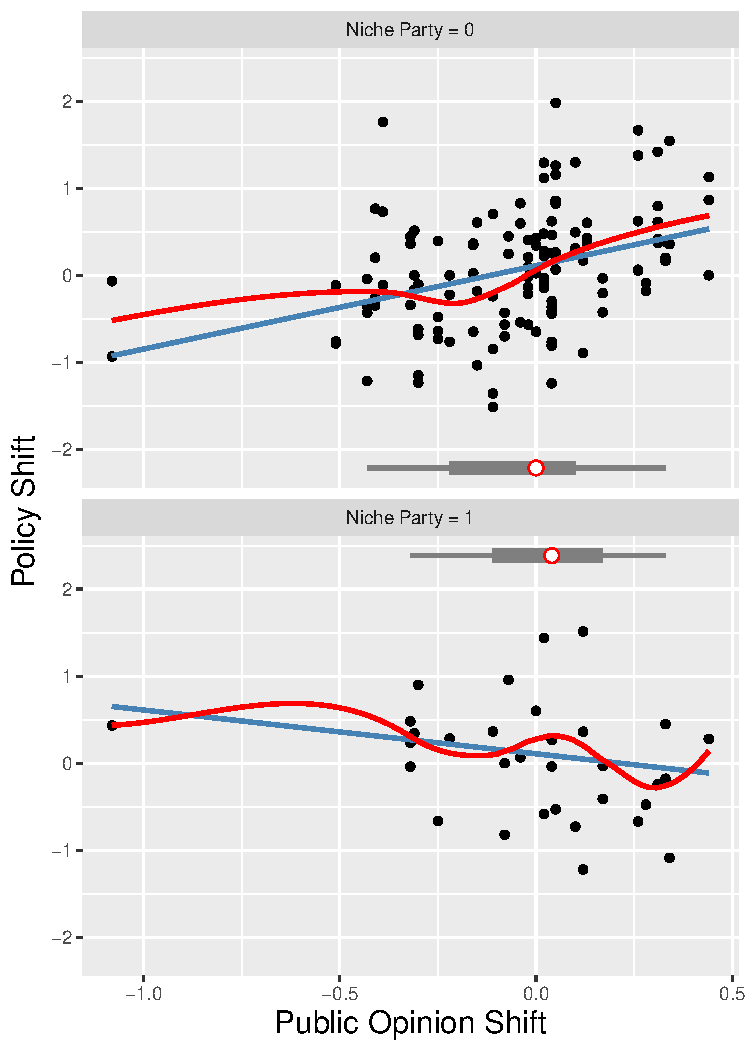
\includegraphics[width=0.5\textwidth]{adams_2006_raw.pdf}}\\
  \subfigure[Marginal Effects from Replicated Model (black line) and from Binning Estimator (white dots)]{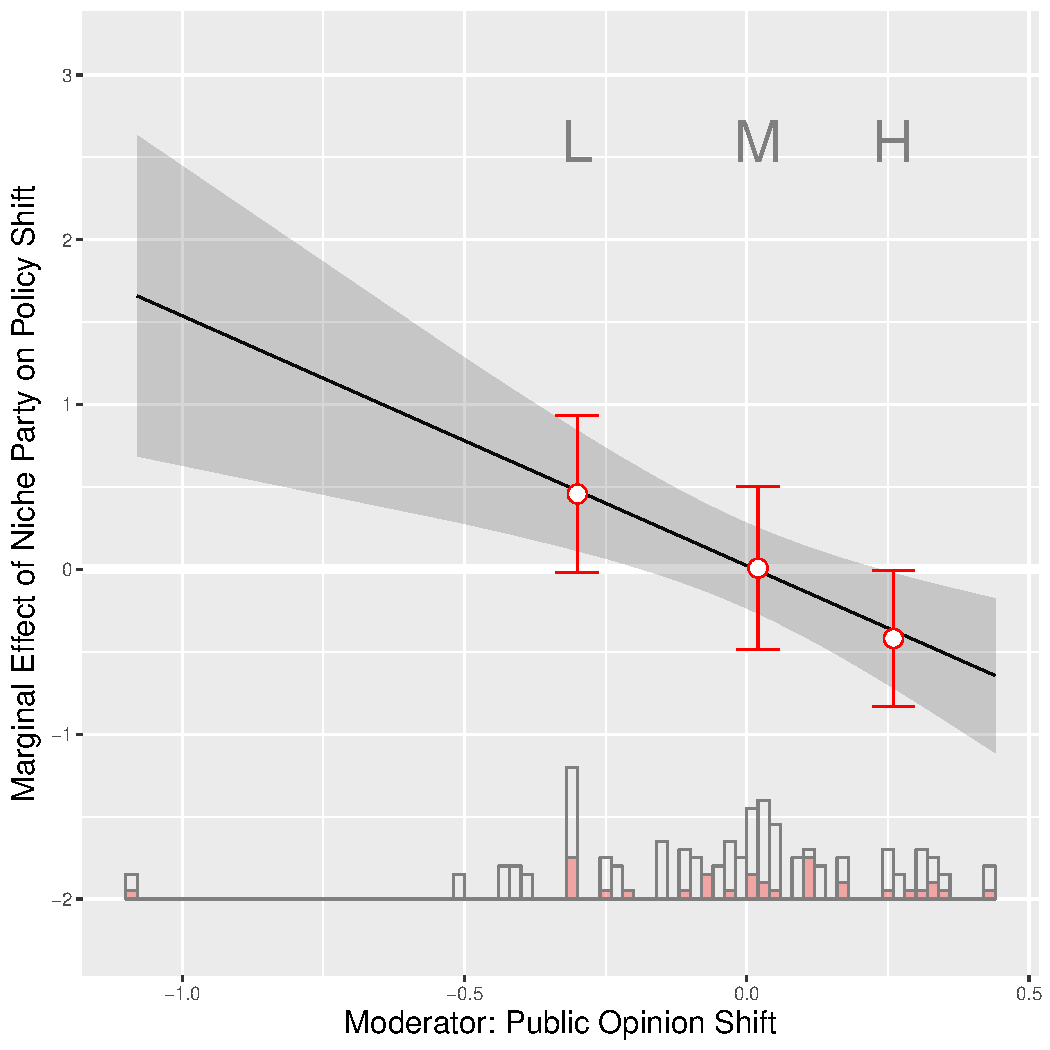
\includegraphics[width=0.45\textwidth]{adams_2006_est0.pdf}}
  \subfigure[Marginal Effects from Kernel Estimator]{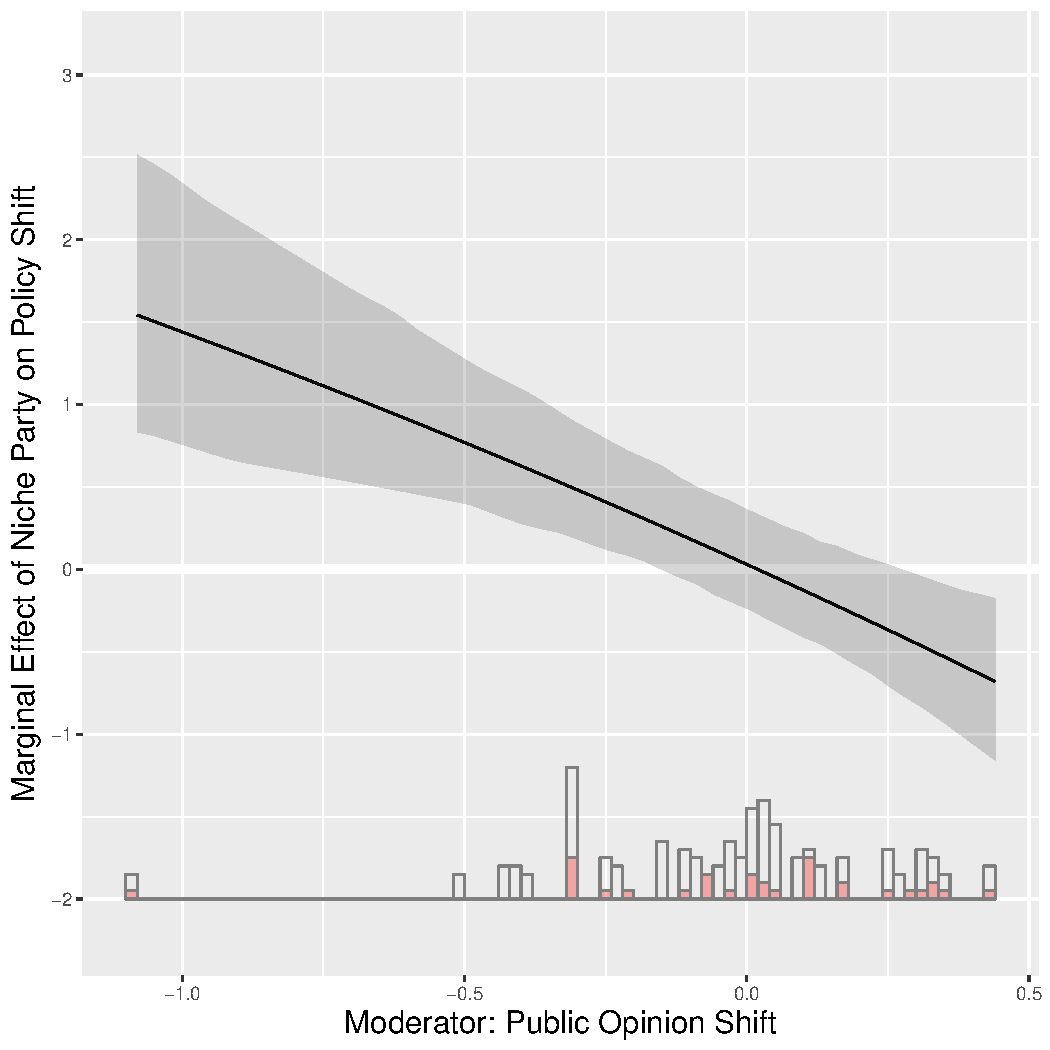
\includegraphics[width=0.45\textwidth]{adams_2006_smooth.pdf}}
\end{figure}%\vspace{-2em}
\clearpage


\subsection{\citet{Aklin2013} AJPS} \label{aklin}

First interaction:

\paragraph{Claim on conditionality (Figure 1, left panel in manuscript):} \emph{``We examine formally how exogenous shocks, such as changes in international energy prices, interact with positive reinforcement factors, such as the growing strength of the renewables advocacy coalition. We find that political competition modifies the effect of path dependence on policy and outcomes. ... The effect of positive reinforcement also decreases with international energy prices.''} (Abstract). 

\paragraph{Key variables for the conditional relationship:} Outcome Y:
``renewable share'' (first differenced) (\texttt{drenew\_capacity\_nh\_share}); treatment D:  ``oil prices'' \\
(\texttt{oilcrude\_price2007dollar\_bp}); moderator X: `lag positive reinforcement'' (\texttt{lrenewpc})
\clearpage

\begin{figure}[!ht]
  \caption{Results from  \citet{Aklin2013}}
  \setcounter{subfigure}{0}
  \centering
  \subfigure[Raw data]{ 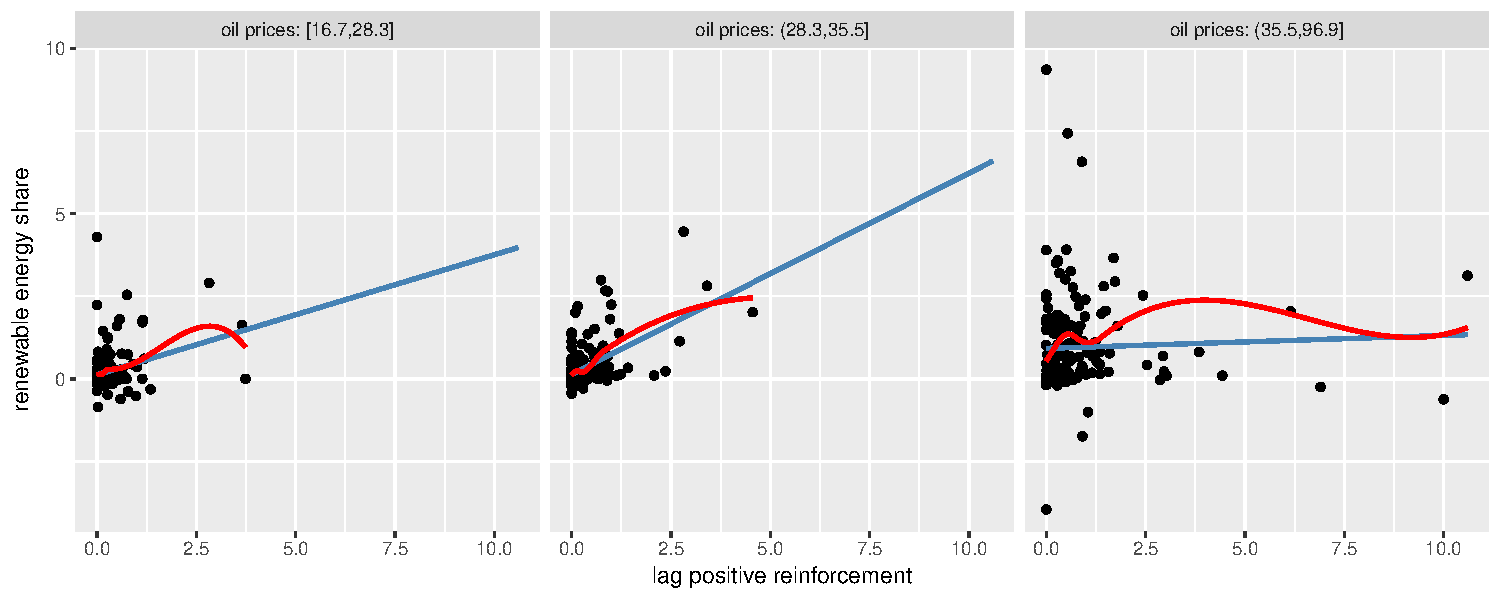
\includegraphics[width=1\textwidth]{aklin_2013b_raw.pdf} }
  \subfigure[GAM Plot] { 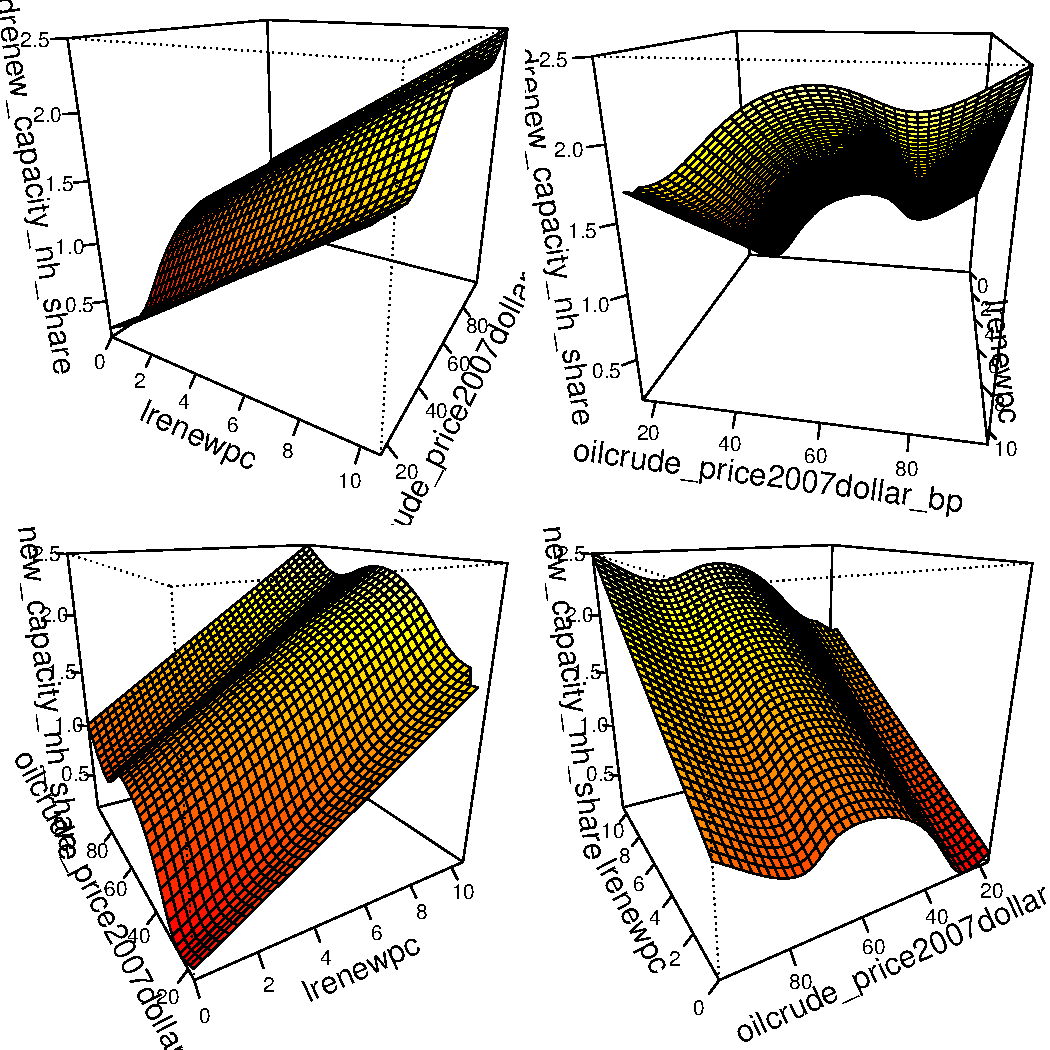
\includegraphics[width=0.45\textwidth]{aklin_2013b_gam.pdf}}\\
  \subfigure[Marginal Effects from Replicated Model (black line) and from Binning Estimator (white dots)]{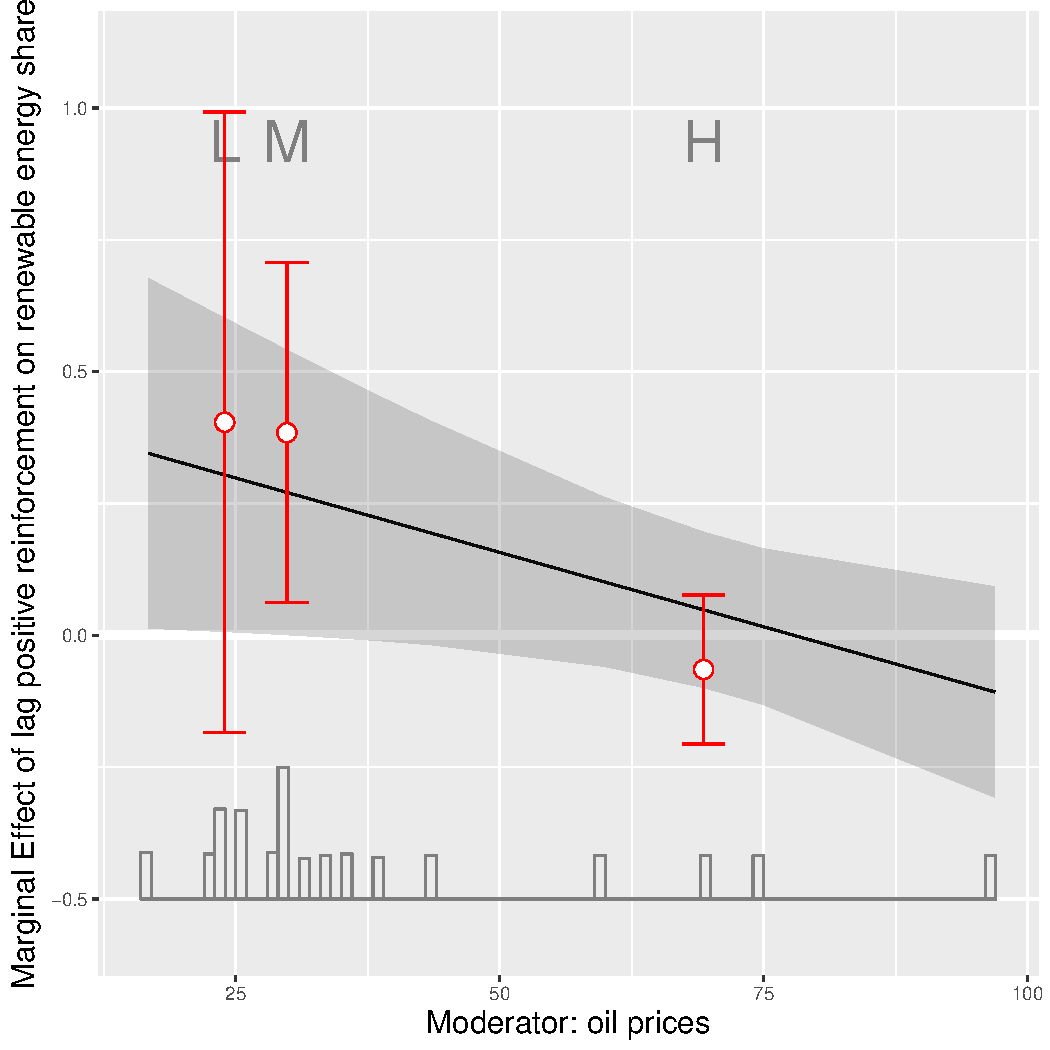
\includegraphics[width=0.45 \textwidth]{aklin_2013b_est0.pdf}}
  \subfigure[Marginal Effects from Kernel Estimator]{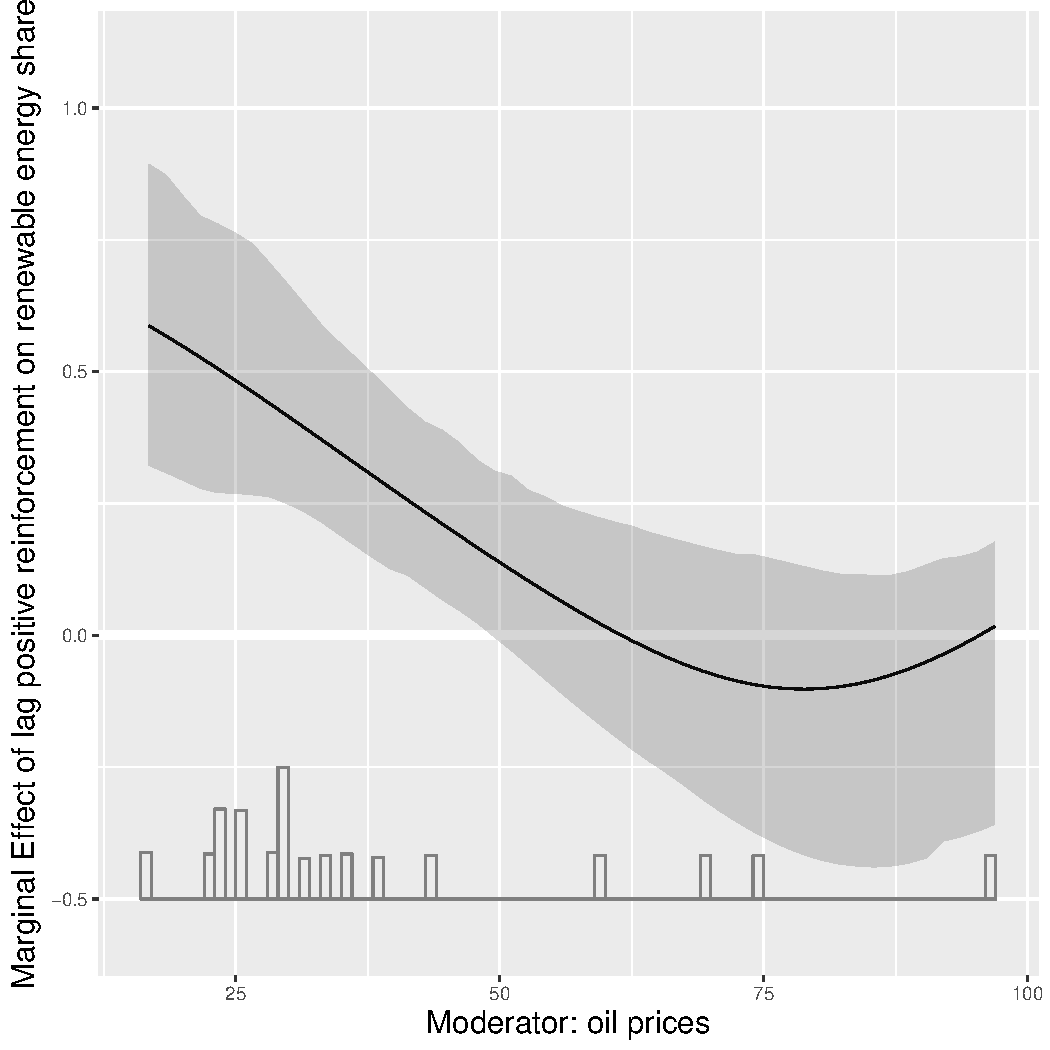
\includegraphics[width=0.45\textwidth]{aklin_2013b_smooth.pdf}}
\end{figure}%\vspace{-2em}
\clearpage

%%%%%%%%%%%%%%%%%%%%%%%% 
\noindent Second interaction:

\paragraph{Claim on conditionality (Figure 1, right panel in manuscript):} \emph{``We examine formally how exogenous shocks, such as changes in international energy prices, interact with positive reinforcement factors, such as the growing strength of the renewables advocacy coalition. We find that political competition modifies the effect of path dependence on policy and outcomes. ... The effect of positive reinforcement also decreases with international energy prices.''} (Abstract). 

\paragraph{Key variables for the conditional relationship:} Outcome Y:
``renewable share'' (first differenced) (\texttt{drenew\_capacity\_nh\_share}); treatment D:  ``lag positive reinforcement'' (\texttt{lrenewpc}); moderator X: ``oil prices'' (\texttt{oilcrude\_price2007dollar\_bp}). 

\paragraph{Note:}  The dashed vertical line indicates the truncated interval of the moderator shown in the original marginal effect plot.
\clearpage

\begin{figure}[!ht]
  \caption{Results from \citet{Aklin2013}}
  \setcounter{subfigure}{0}
  \centering
  \subfigure[Raw data]{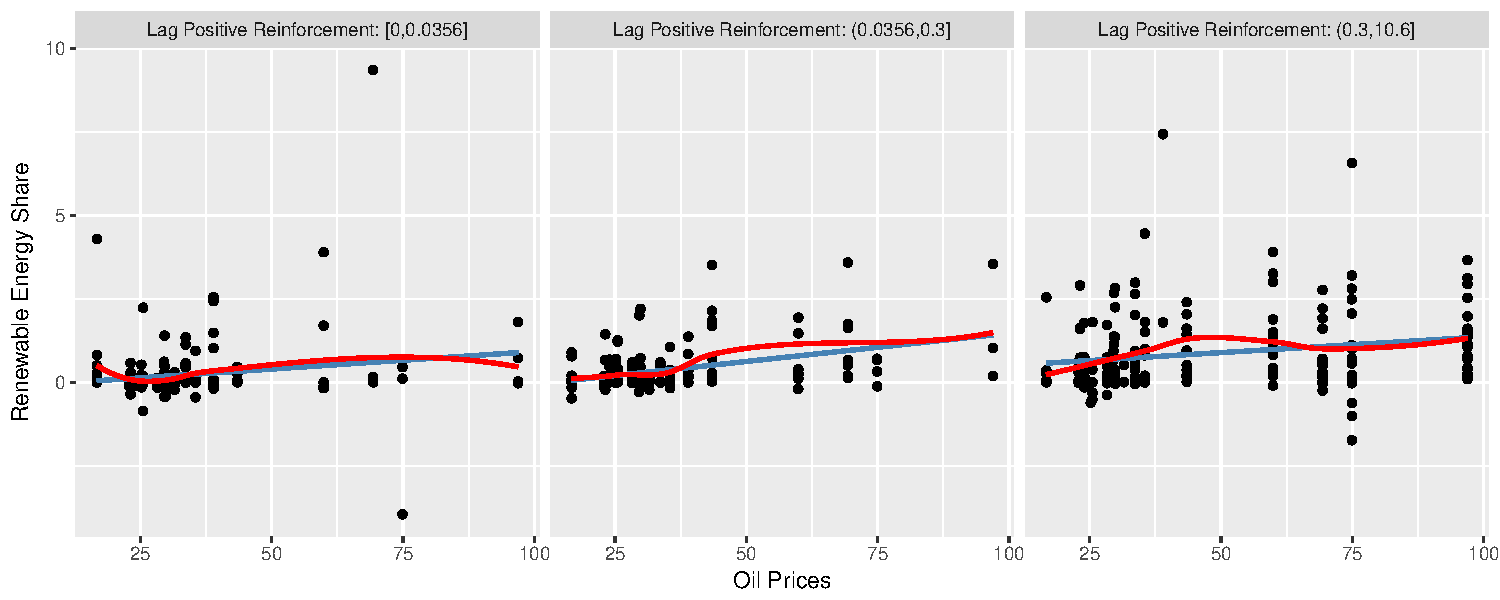
\includegraphics[width=1\textwidth]{aklin_2013a_raw.pdf} }
  \subfigure[GAM]  {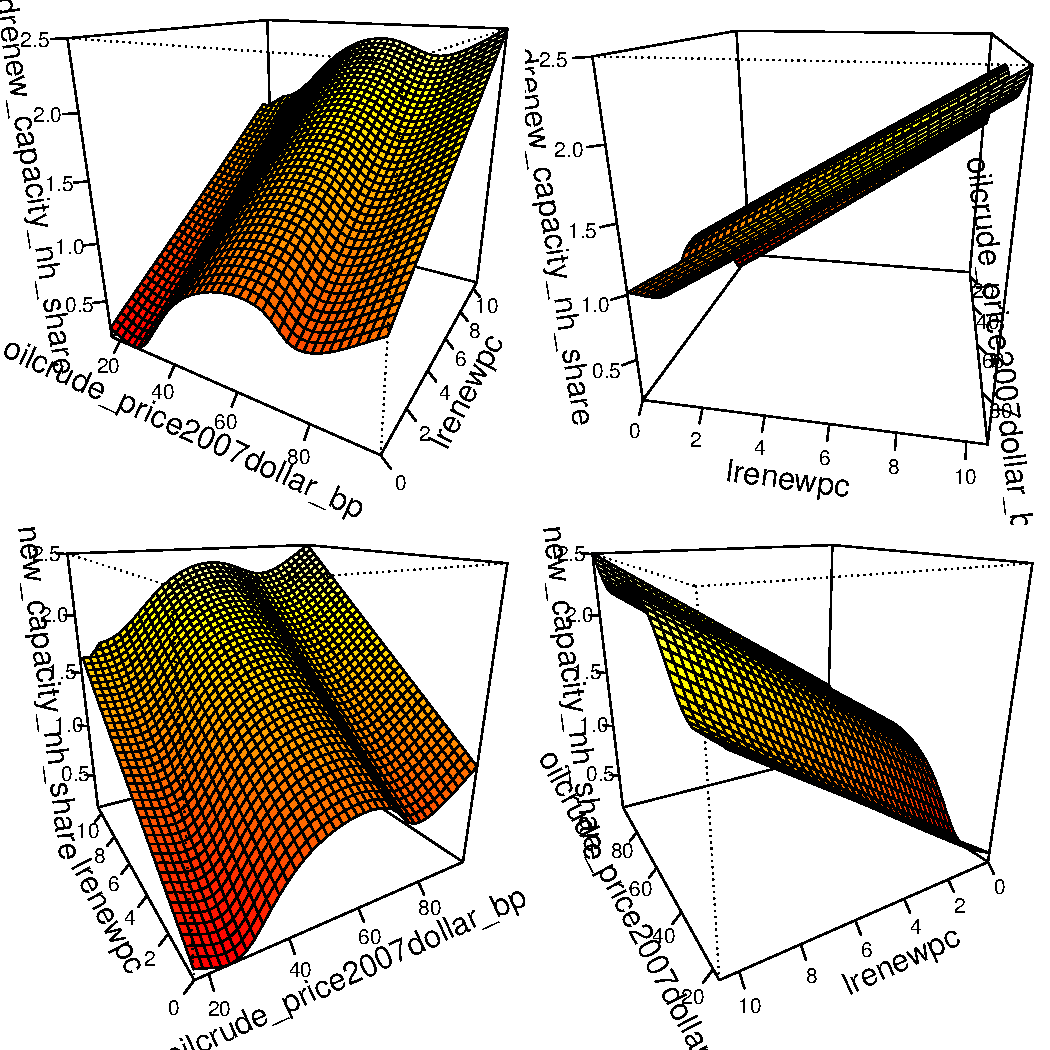
\includegraphics[width=0.45\textwidth]{aklin_2013a_gam.pdf}}\\
  \subfigure[Marginal Effects from Replicated Model (black line) and from Binning Estimator (white dots)]{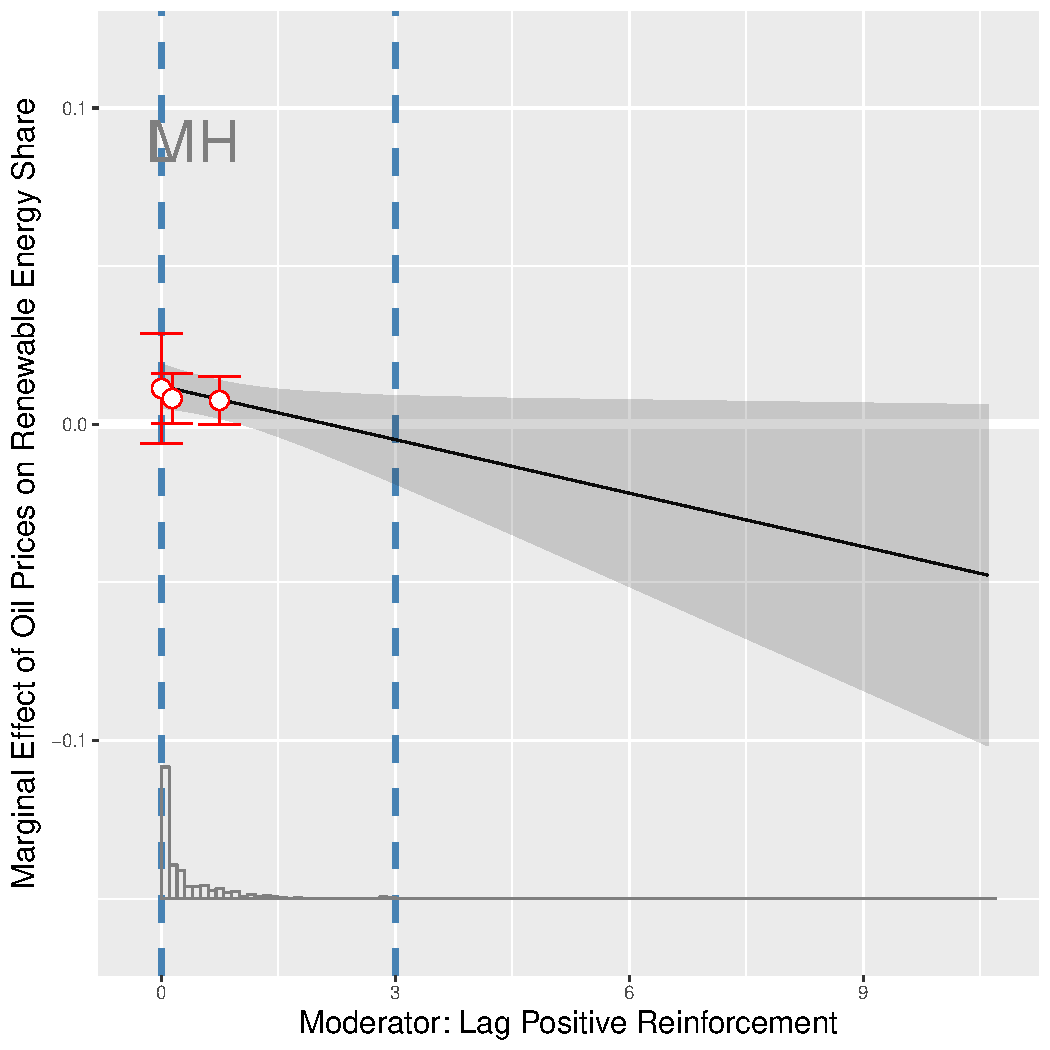
\includegraphics[width=0.45\textwidth]{aklin_2013a_est0.pdf}}
  \subfigure[Marginal Effects from Kernel Estimator]{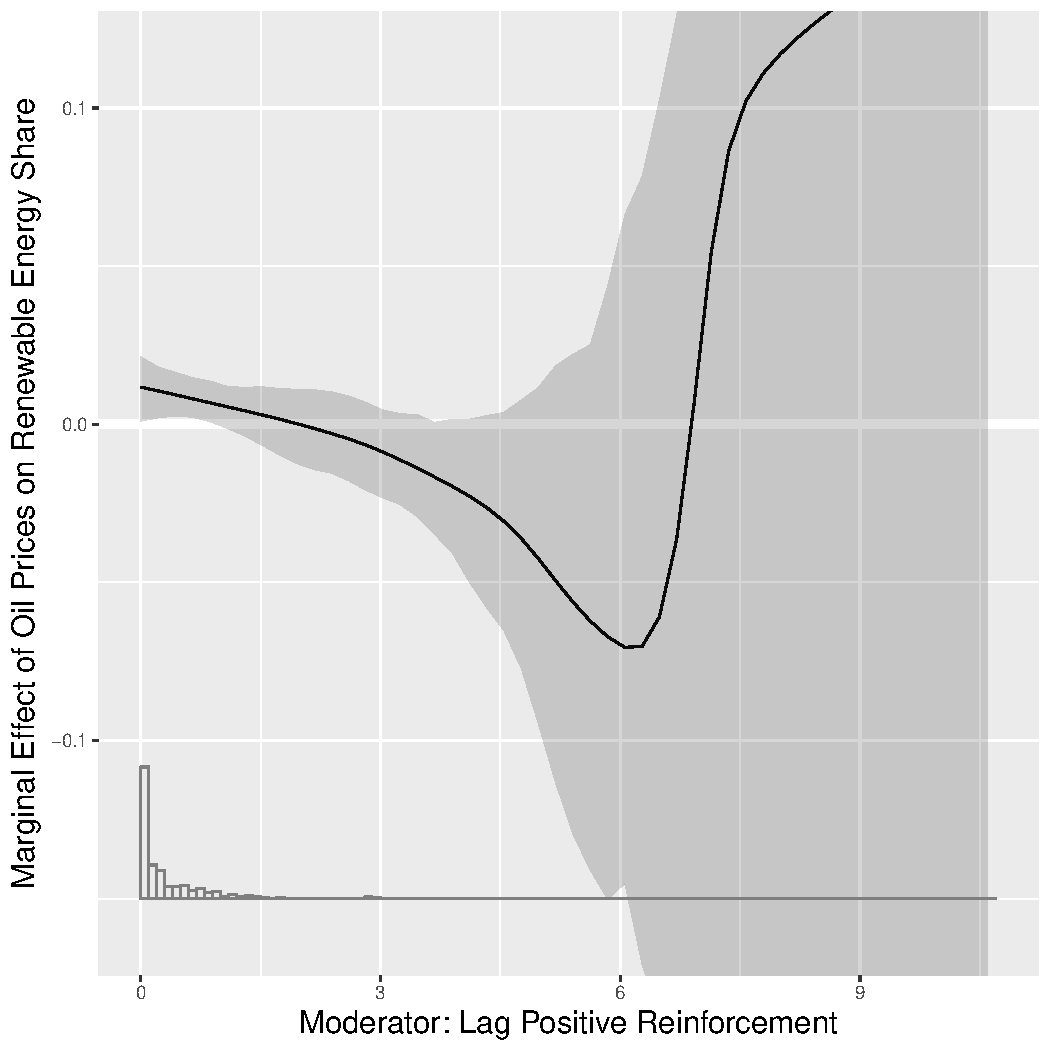
\includegraphics[width=0.45\textwidth]{aklin_2013a_smooth.pdf}}
\end{figure}%\vspace{-2em}
\clearpage



\subsection{\citet{Banks2012} AJPS} \label{banks}

First interaction:


\paragraph{Claim on conditionality (Figure 1 in manuscript):} \emph{``One explanation for this is that a new racial belief system referred to as symbolic racism or racial resentment has replaced `old-fashioned racism.' ... as a result, anger now serves as the primary emotional trigger of whites' negative racial attitudes''} (Abstract).

\emph{``Figure 1 illustrates the marginal effect of each emotion on racial policy opinions across levels of symbolic racism (SR) ... As we predict, as SR increases, anger increasingly boosts opposition to racial policies such as affirmative action''} (p. 292).

\paragraph{Key variables for conditional relationship:} Outcome Y: ``policy opinion'' (\texttt{racpolicy}); treatment D: ``anger'' (\texttt{anger}); moderator X: ``symbolic racism'' (\texttt{racresent1}).

\paragraph{Note:} Due to coding errors in the authors' original analysis, the marginal effects plots we present here feature different intercepts than those in the published paper We corrected the errors before applying our diagnostic functions.


\clearpage

%%%%%%%%%%%%%%%%%%%%%%%% 



\begin{figure}[!ht]
  \caption{Results from  \citet{Banks2012} }
  \setcounter{subfigure}{0}
  \centering
 \subfigure[Raw data]  {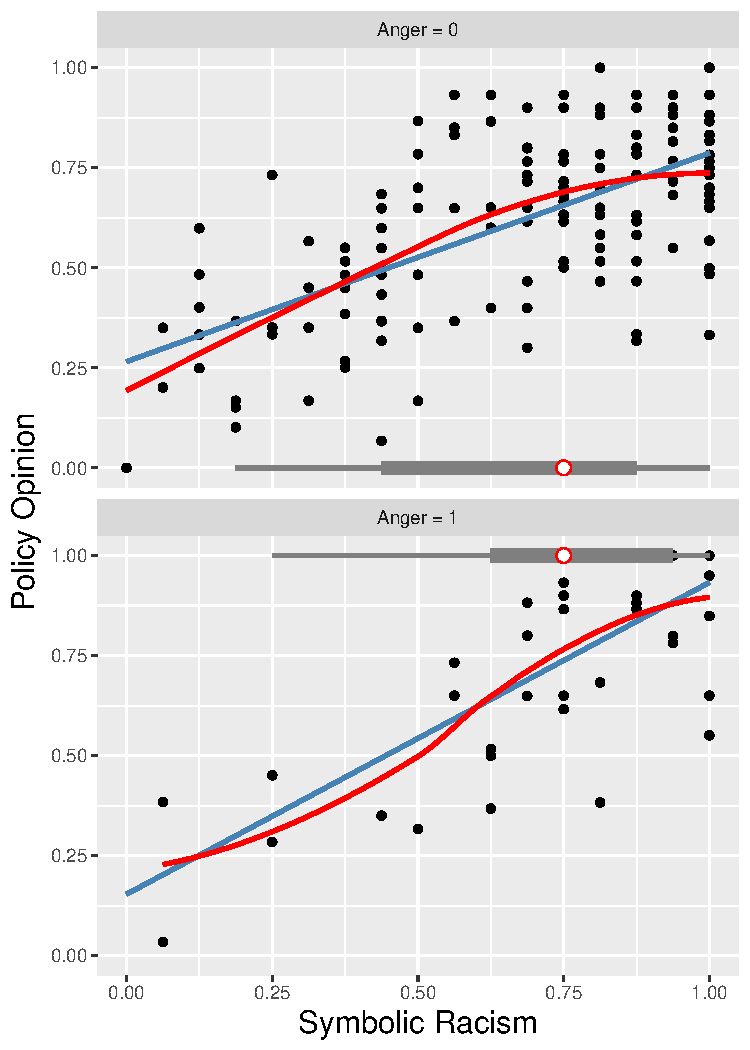
\includegraphics[width=0.5\textwidth]{banks_2012a_raw.pdf} }\\
  \subfigure[Marginal Effects from Replicated Model (black line) and from Binning Estimator (white
dots)]{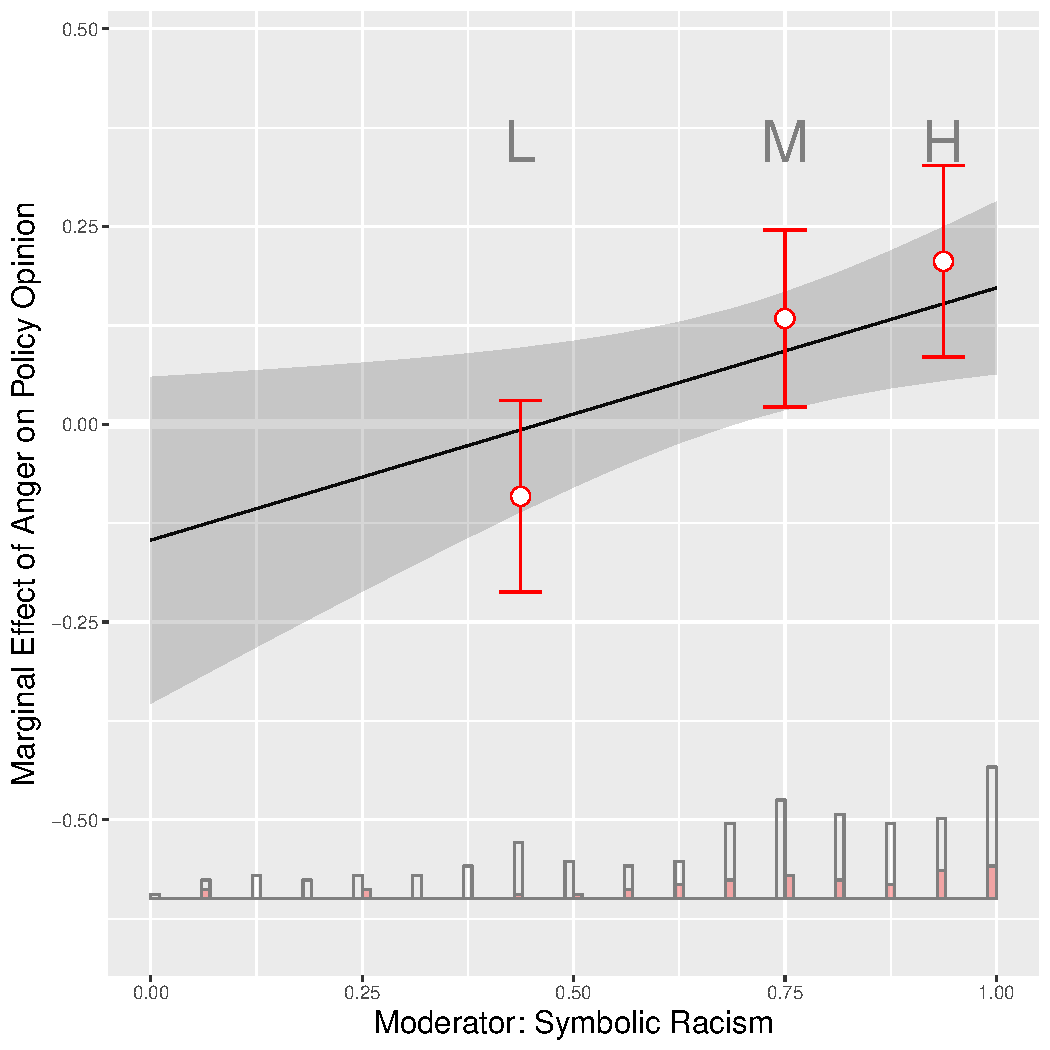
\includegraphics[width=0.45\textwidth]{banks_2012a_est0.pdf}}
  \subfigure[Marginal Effects from Kernel Estimator]{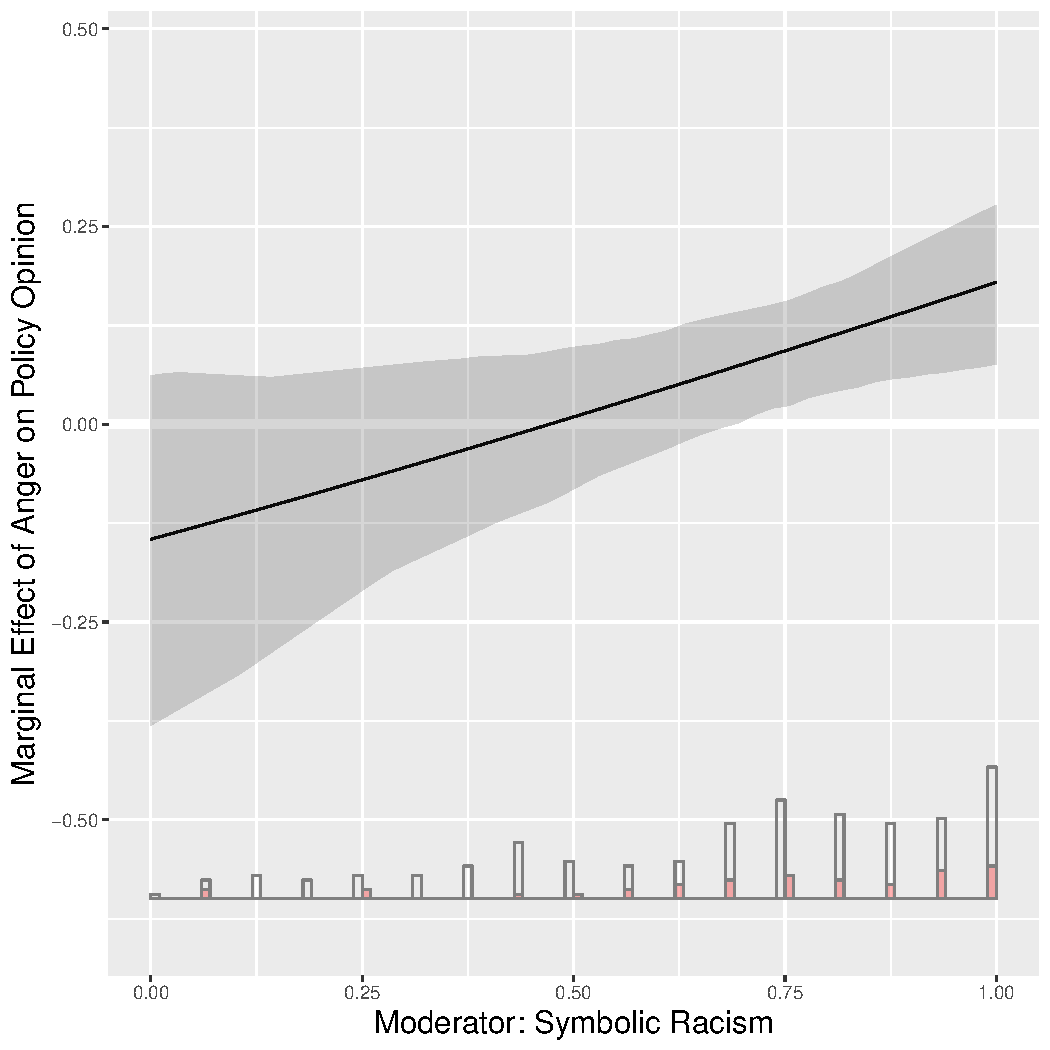
\includegraphics[width=0.45\textwidth]{banks_2012a_smooth.pdf}}
\end{figure}%\vspace{-2em}
\clearpage

%%%%%%%%%%%%%%%%%%%%%%%% 
\noindent Second interaction:



\paragraph{Claim on conditionality (Figure
  2 in manuscript):} \emph{``Figure 2 displays these interactions visually and shows
that the effects of anger and disgust are larger than that
of fear, but these differences are not as large or statistically
distinct. However, as OFR increases, both anger
and disgust boost opposition to racial policies. At very
high levels of OFR, both anger and disgust boost opposition
significantly more than that in the (relaxed) control
group."} (p. 292)

\paragraph{Key variables for conditional relationship:} Outcome Y:
``policy opinion'' (\texttt{racpolicy}); treatment D: ``anger'' (\texttt{anger}); moderator X: ``old-fashioned racism'' (\texttt{jimcrow13}).

\clearpage
 
\begin{figure}[!ht]
  \caption{Results from  \citet{Banks2012} }
  \setcounter{subfigure}{0}
  \centering
  \subfigure [Raw data]{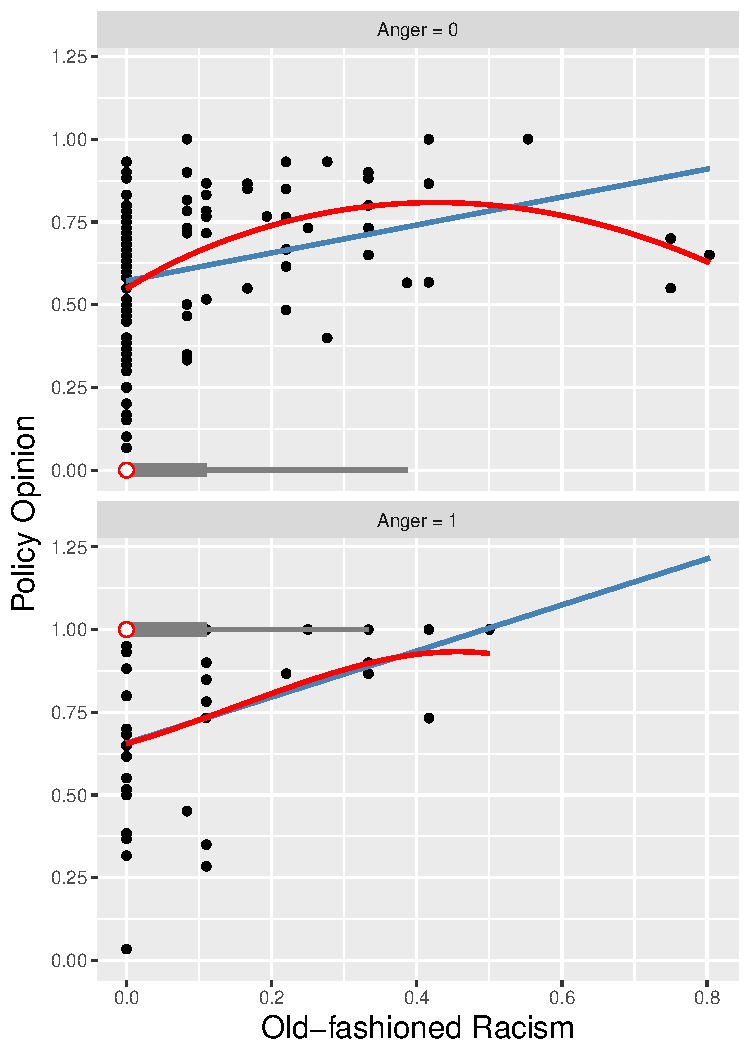
\includegraphics[width=0.5\textwidth]{banks_2012b_raw.pdf} }\\
  \subfigure[Marginal Effects from Replicated Model (black line) and from Binning Estimator (white
dots)]{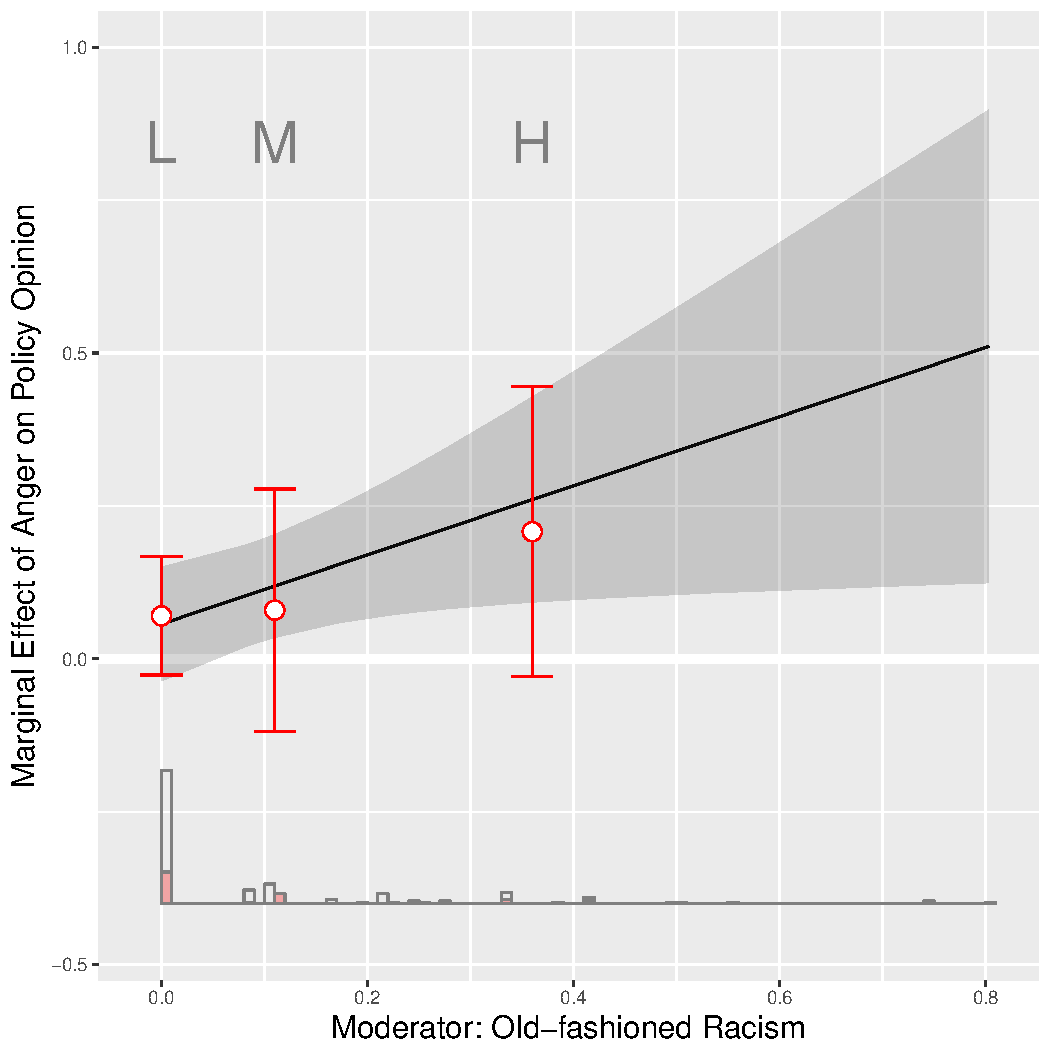
\includegraphics[width=0.45\textwidth]{banks_2012b_est0.pdf}}
  \subfigure[Marginal Effects from Kernel Estimator]{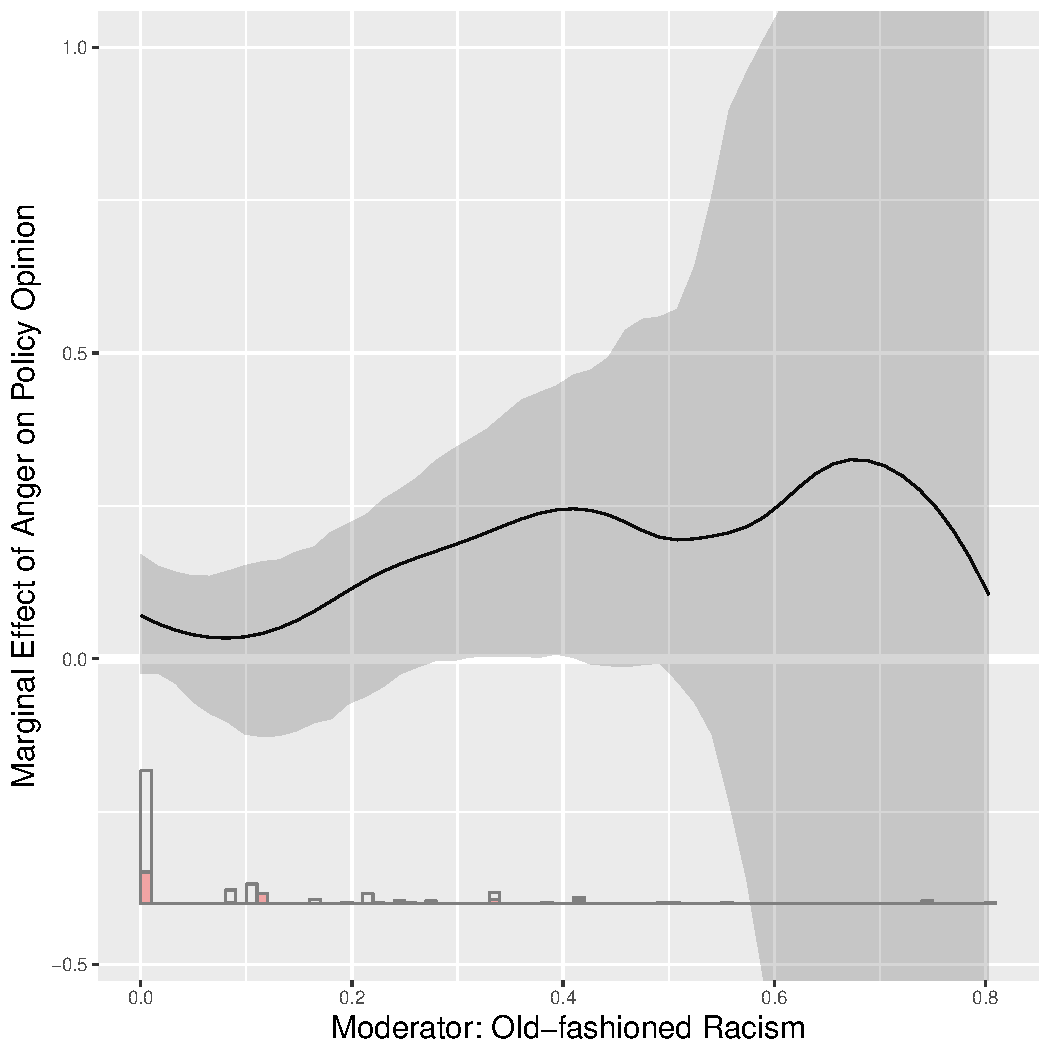
\includegraphics[width=0.45\textwidth]{banks_2012b_smooth.pdf}}
\end{figure}%\vspace{-2em}
\clearpage


%%%%%%%%%%%%%%%%%%%%%%%% 
\noindent Third interaction:

\paragraph{Claim on conditionality (Figure
  2 in manuscript):} \emph{``Figure 2 displays these interactions visually and shows
that the effects of anger and disgust are larger than that
of fear, but these differences are not as large or statistically
distinct. However, as OFR increases, both anger
and disgust boost opposition to racial policies. At very
high levels of OFR, both anger and disgust boost opposition
significantly more than that in the (relaxed) control
group.''} (p. 292)

\paragraph{Key variables for conditional relationship:} Outcome Y:
``policy opinion'' (\texttt{racpolicy}); treatment D: ``disgust'' (\texttt{disgust}); moderator X: ``old-fashioned racism'' (\texttt{jimcrow13}).


\clearpage


\begin{figure}[!ht]
  \caption{Results from  \citet{Banks2012} }
  \setcounter{subfigure}{0}
  \centering
  \subfigure[Raw data] {  \centering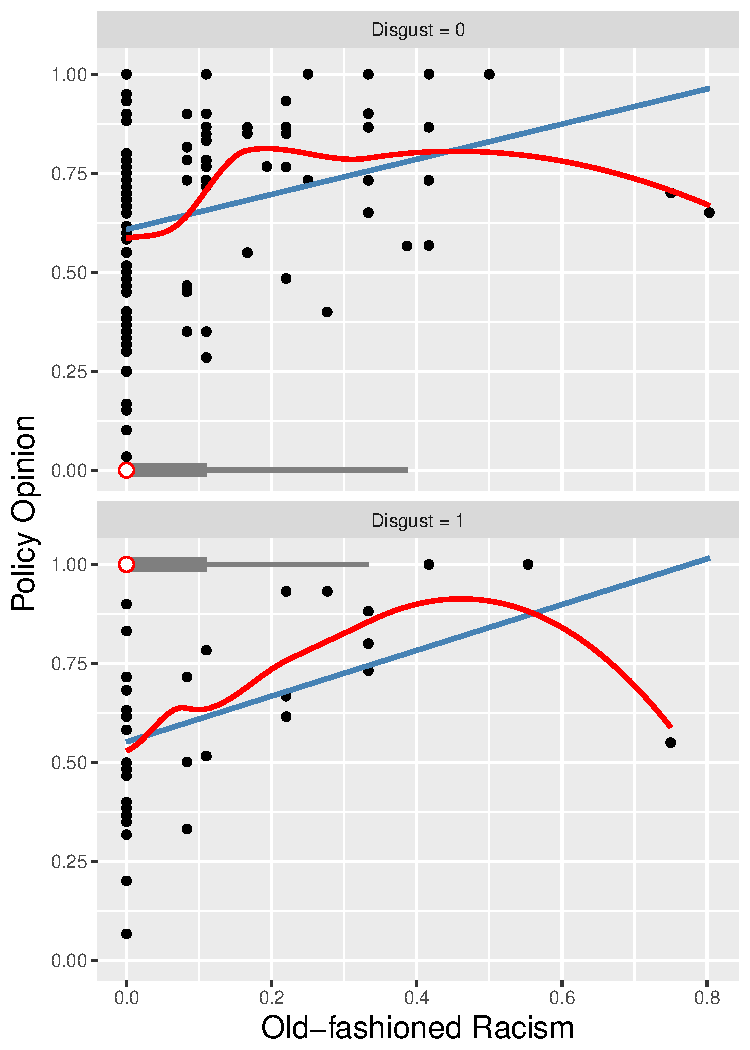
\includegraphics[width=0.5\textwidth]{banks_2012c_raw.pdf} }\\
  \subfigure[Marginal Effects from Replicated Model (black line) and from Binning Estimator (white
dots)]{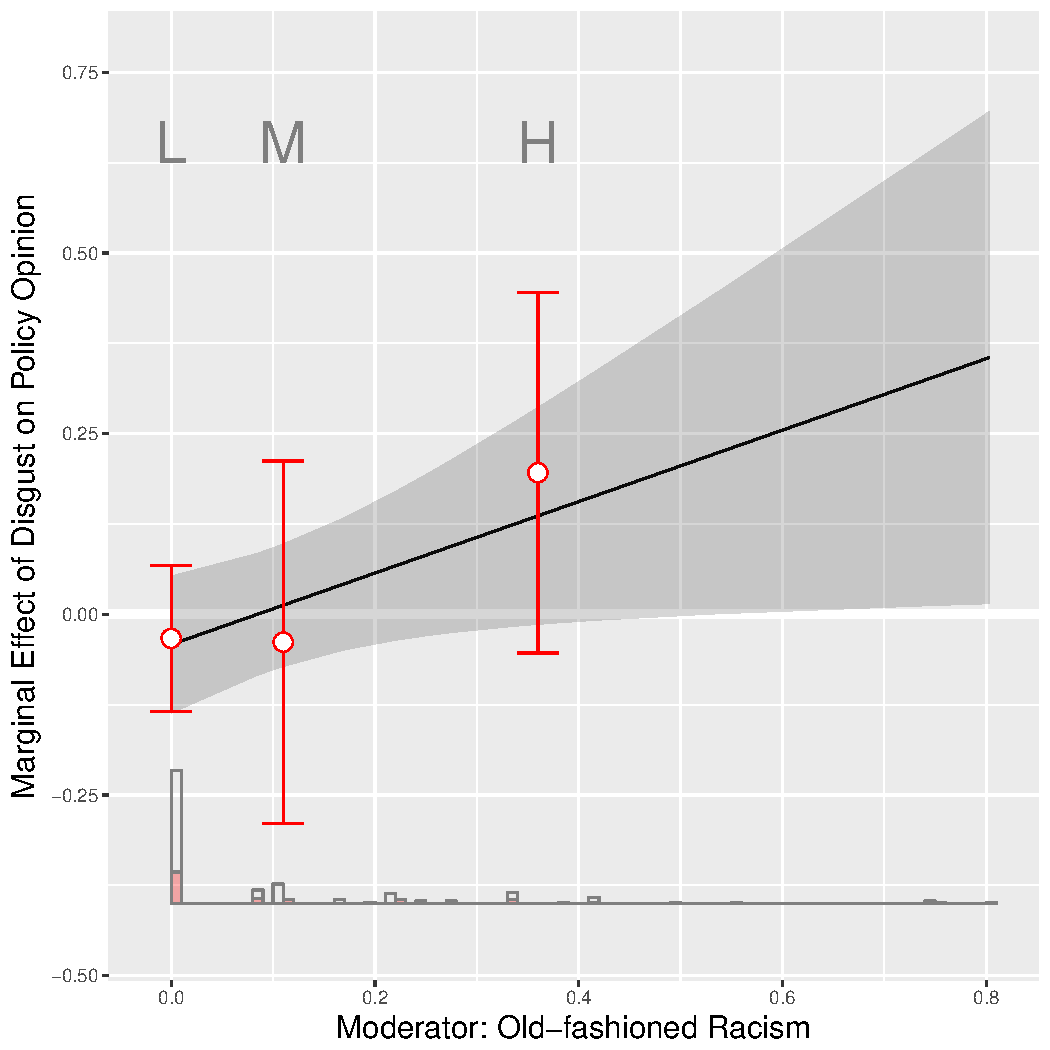
\includegraphics[width=0.45\textwidth]{banks_2012c_est0.pdf}}
  \subfigure[Marginal Effects from Kernel Estimator]{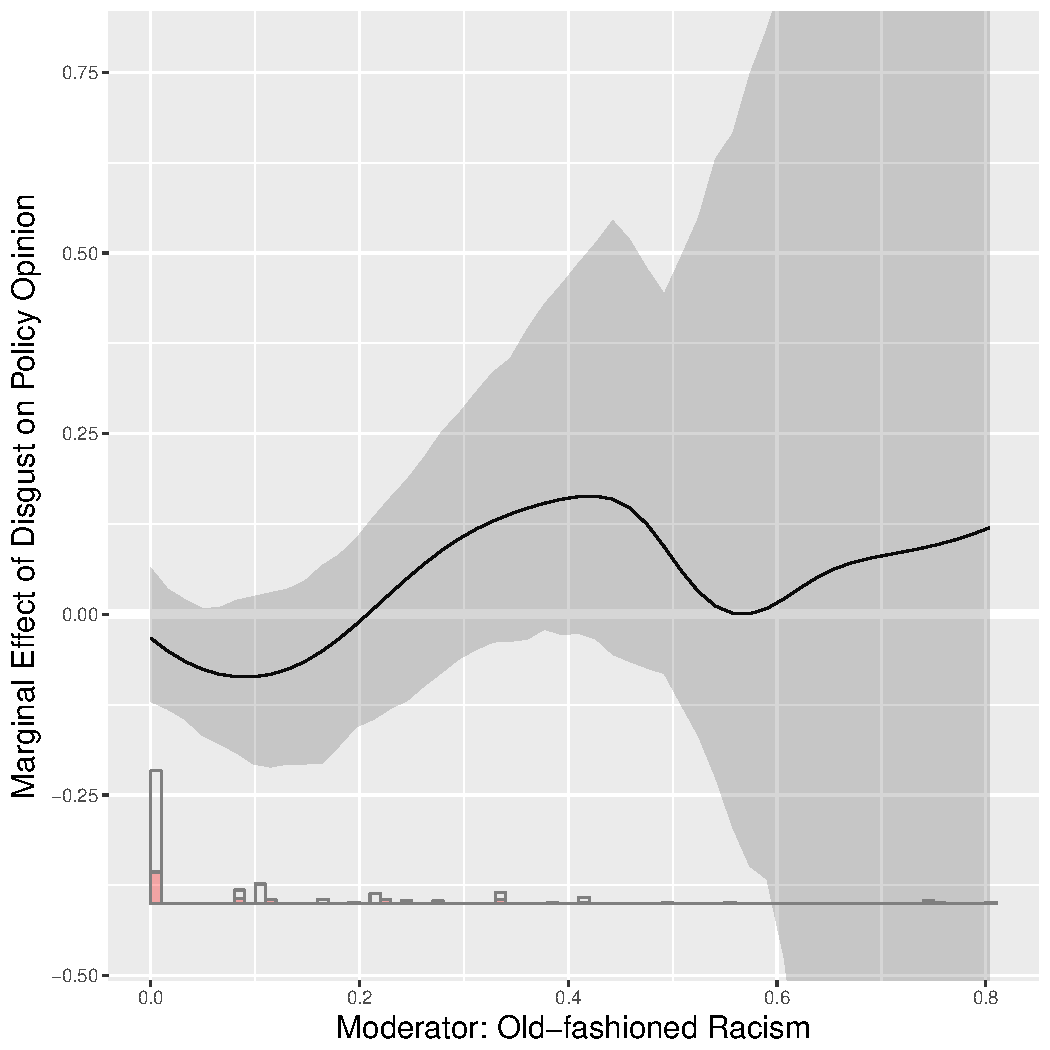
\includegraphics[width=0.45\textwidth]{banks_2012c_smooth.pdf}}
\end{figure}
\clearpage




\subsection{\citet{Bodea2015_JOP} JOP} \label{bodea_JOP}

First interaction:

\paragraph{Claim on conditionality  (Figure 1a in manuscript):}  \emph{``In addition, we show that CBI affects the flow and cost of capital in non-OECD countries ... where political institutions allow
  the central bank to de facto be credible.''} (Abstract).

\emph{``We plot the marginal effect of CBI as democracy increases in
  non-OECD countries in Figure 1(a). The marginal effect is
  significant only at high levels of Polity, supporting Hypothesis
  2.1''} (p. 278). 

\paragraph{Key variables for the conditional relationship:} Outcome Y:
``FDI'' (\texttt{fdiinflow}, demeaned); treatment D: ``lag CBI''' (\texttt{llvaw}); moderator X: ``Polity'' (\texttt{polity2\_cen}). 

\paragraph{Note:} The authors show 90\% confidence intervals in the paper, while in both the binning plot and the kernel smoothing plot, we use 95\% confidence intervals.

\clearpage




\begin{figure}[!ht]
  \caption{Results from \citet{Bodea2015_JOP} }
  \setcounter{subfigure}{0}
  \centering
    \subfigure[Raw data]{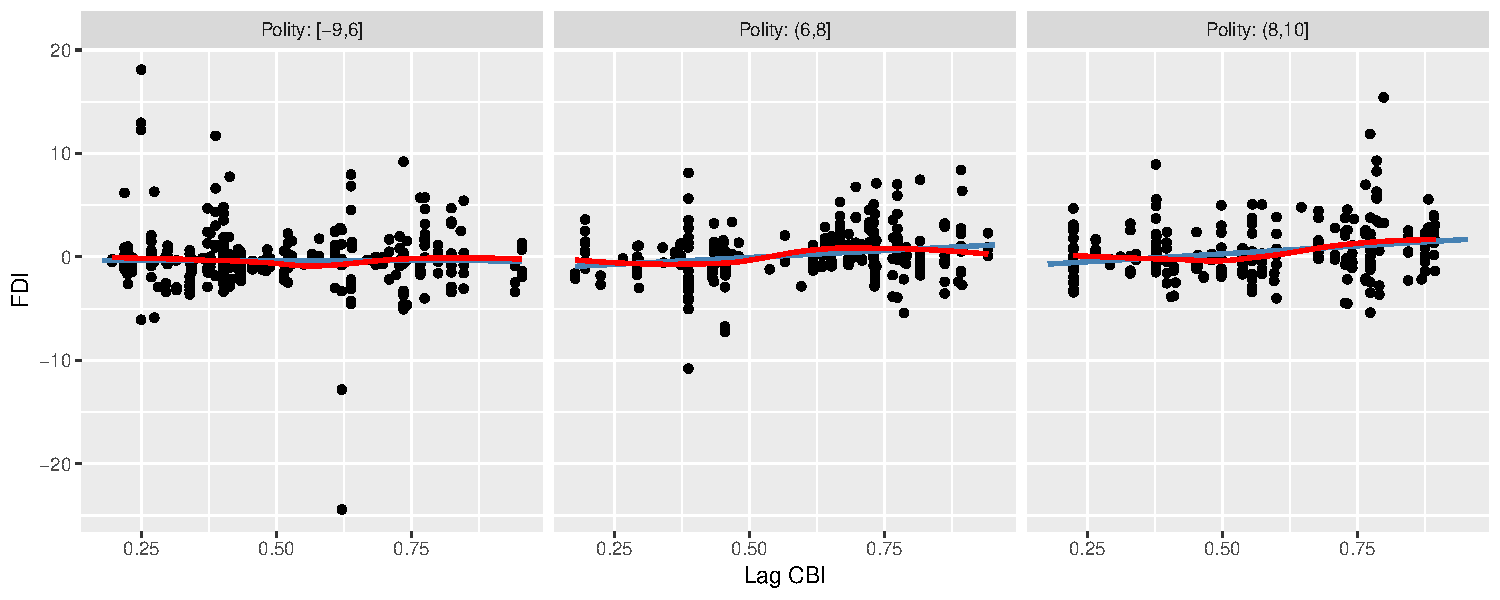
\includegraphics[width=1\textwidth]{bodea_2015a_raw.pdf} }
    \subfigure[GAM] {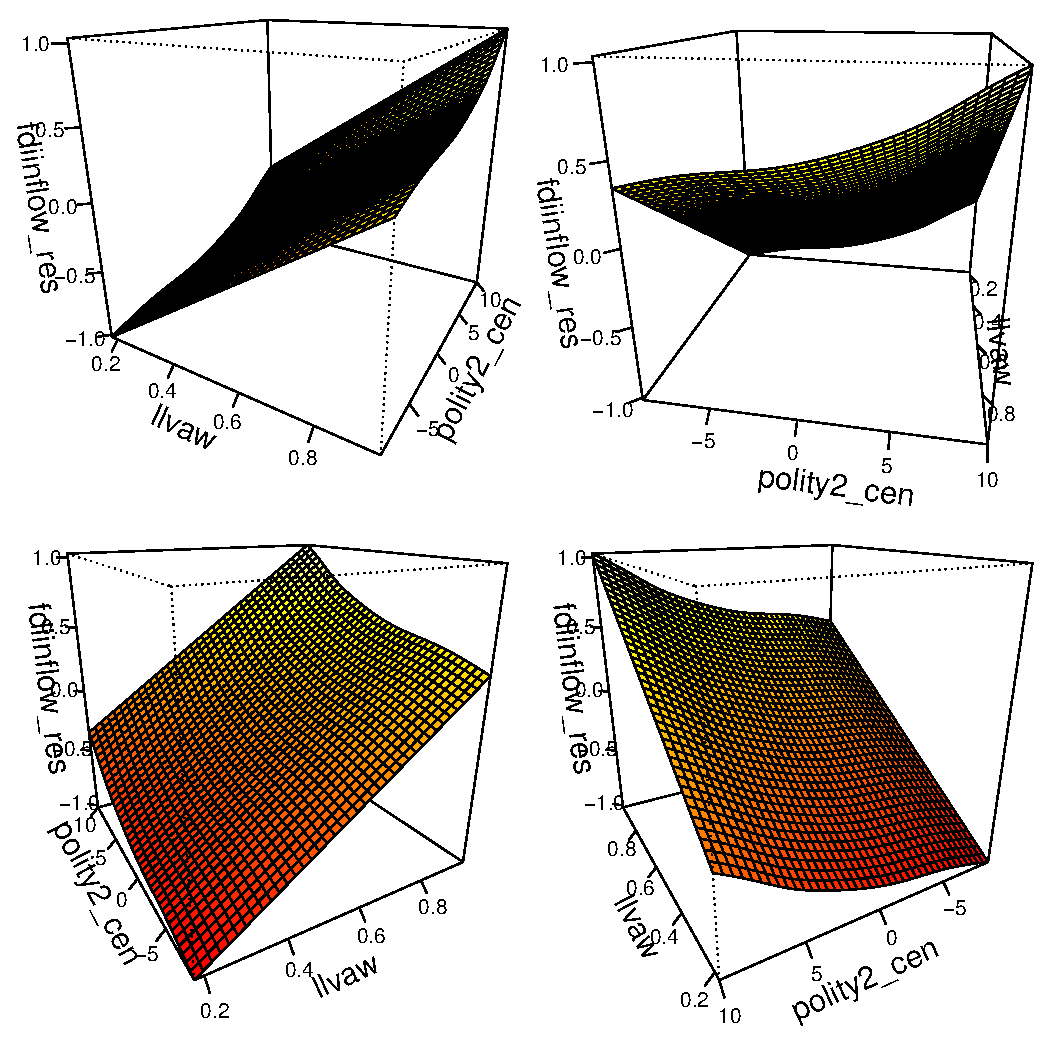
\includegraphics[width=0.45\textwidth]{bodea_2015a_gam.pdf}}\\
  \subfigure[Marginal Effects from Replicated Model (black line) and from Binning Estimator (white
dots)]{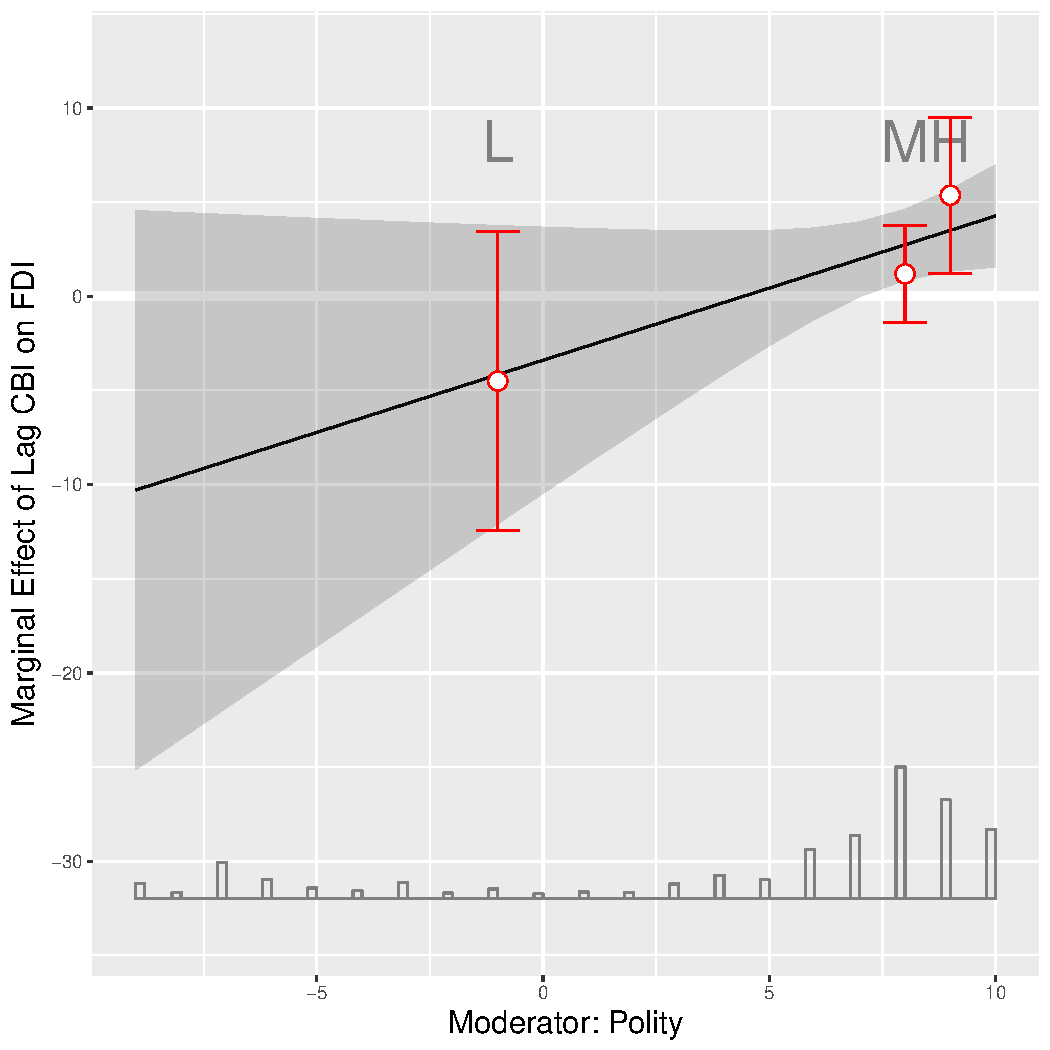
\includegraphics[width=0.45\textwidth]{bodea_2015a_est0.pdf}}
  \subfigure[Marginal Effects from Kernel Estimator]{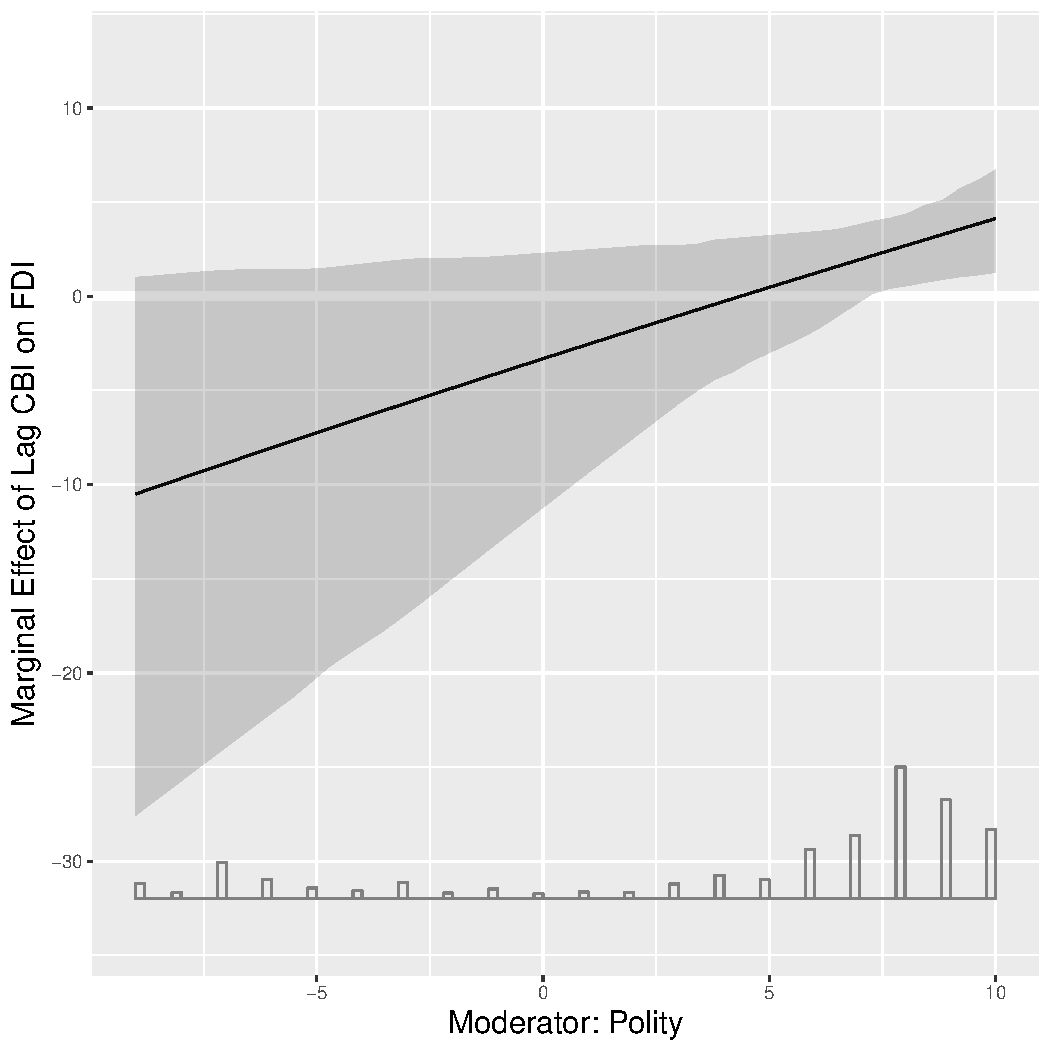
\includegraphics[width=0.45\textwidth]{bodea_2015a_smooth.pdf}}
\end{figure}
\clearpage


\noindent Second interaction:

\paragraph{Claim on conditionality:} \emph{Figure 1(c) shows that the marginal effect
of CBI is downward sloping and negative at higher levels
of democracy. For the 10-year bonds, more independent
central banks reduce borrowing costs for democratic governments
but have no effect in nondemocracies.} (p.\ 279)

\paragraph{Key variables for the conditional relationship (Figure 1c):} Outcome Y: ``10-year bond rates '' (\texttt{real\_10yrate}, demeaned); treatment D: ``lag CBI'' (\texttt{llvaw}); moderator X: ``Polity'' (\texttt{polity2\_cen}). 

\paragraph{Note:} The authors show 90\% confidence intervals in the paper, while in both the binning plot and the kernel smoothing plot, we use 95\% confidence intervals.

\begin{figure}[!ht]
  \caption{Results from \citet{Bodea2015_JOP} }
  \setcounter{subfigure}{0}
  \centering
  \subfigure[Raw data]{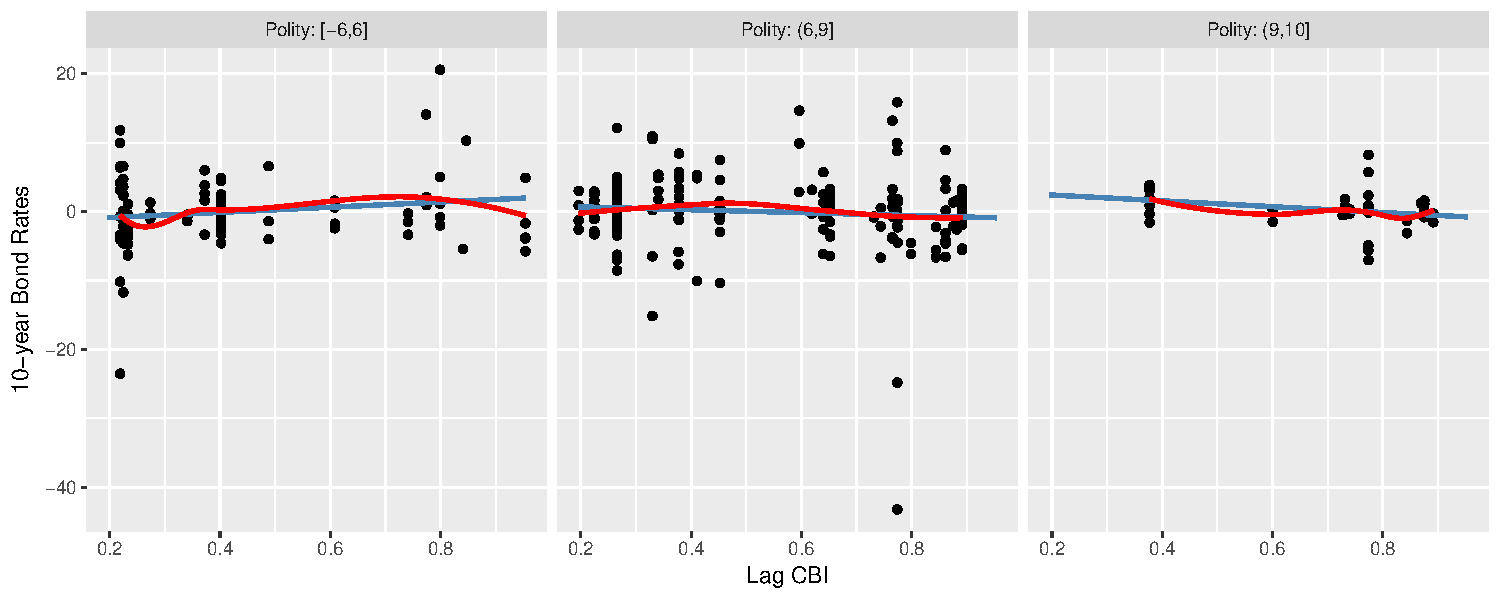
\includegraphics[width=1\textwidth]{bodea_2015b_raw.pdf} }
  \subfigure[GAM]{  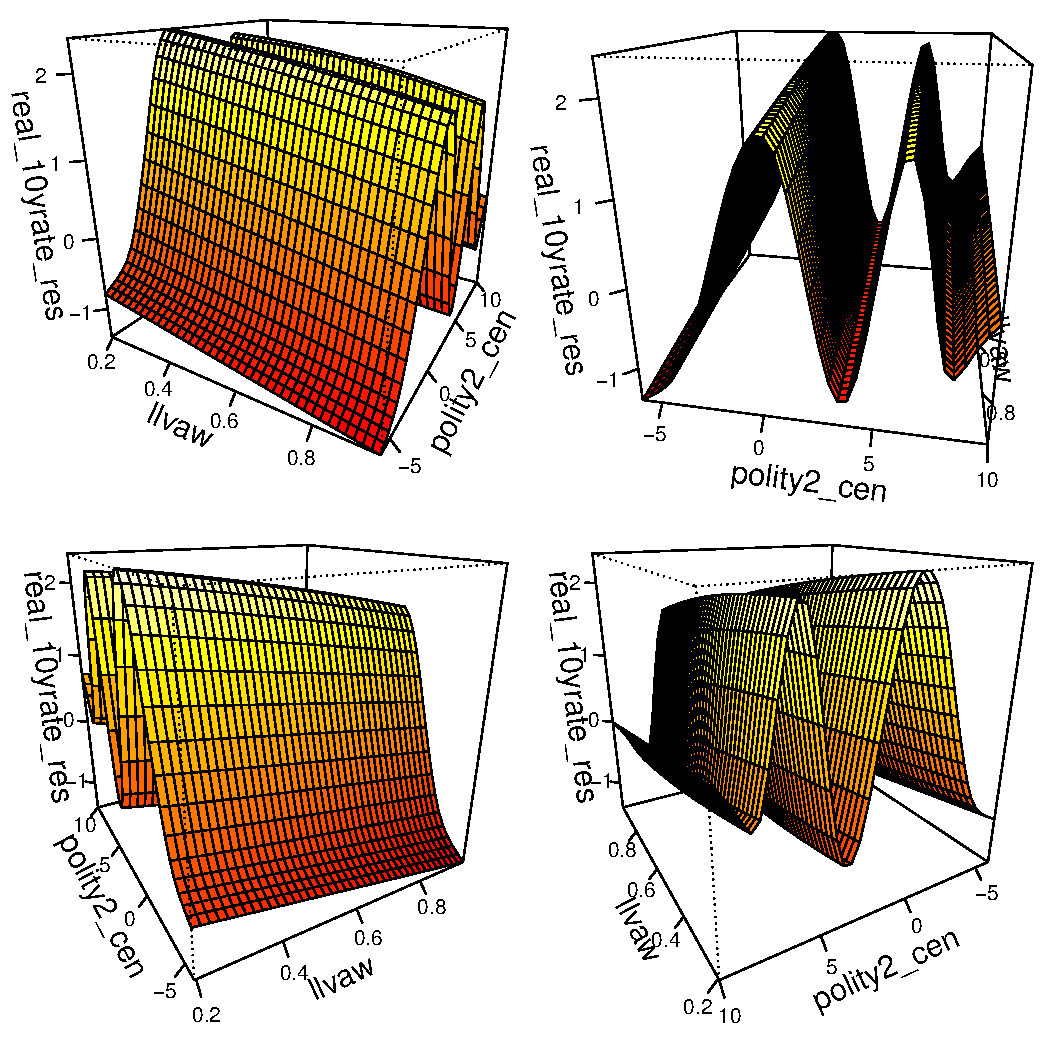
\includegraphics[width=0.45\textwidth]{bodea_2015b_gam.pdf}}\\
  \subfigure[Marginal Effects from Replicated Model (black line) and from Binning Estimator (white
dots)]{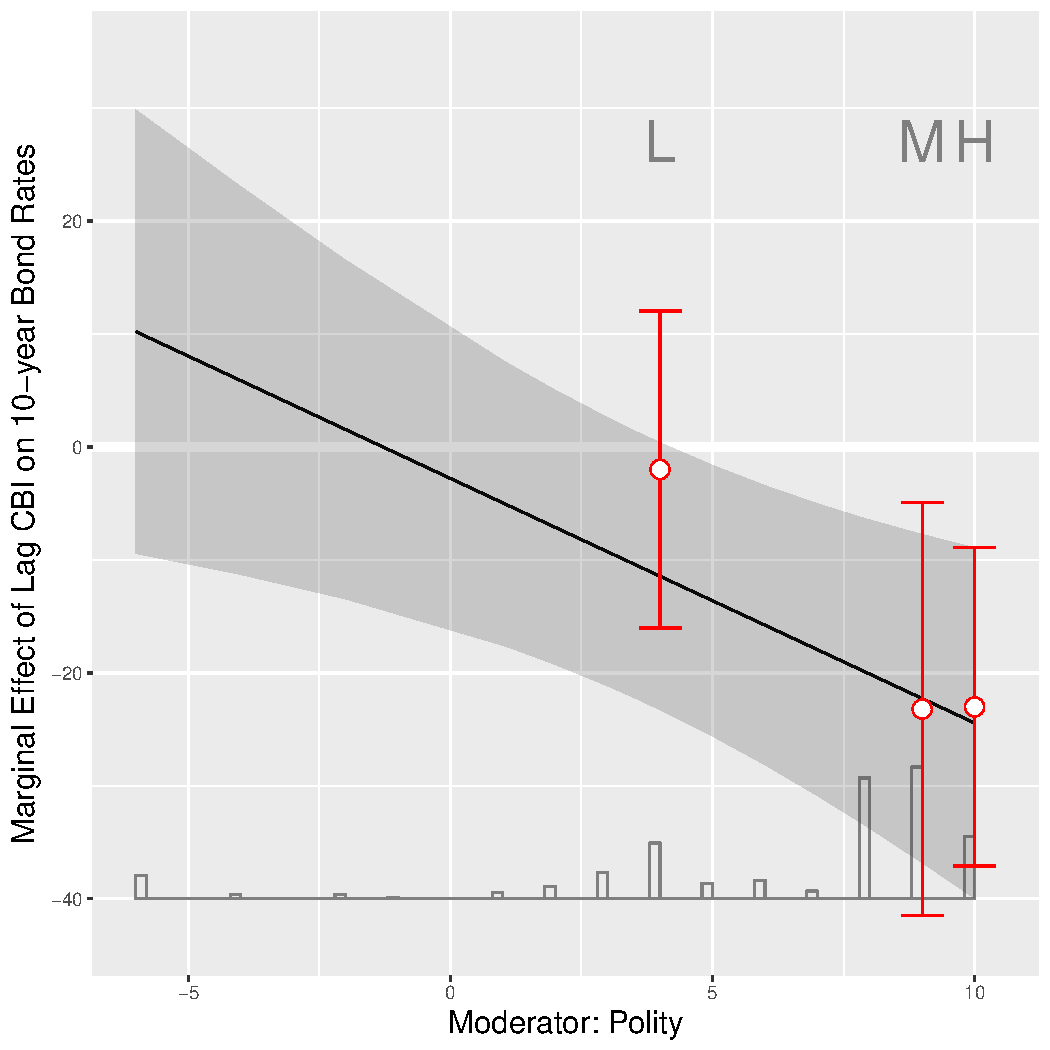
\includegraphics[width=0.45\textwidth]{bodea_2015b_est0.pdf}}
  \subfigure[Marginal Effects from Kernel Estimator]{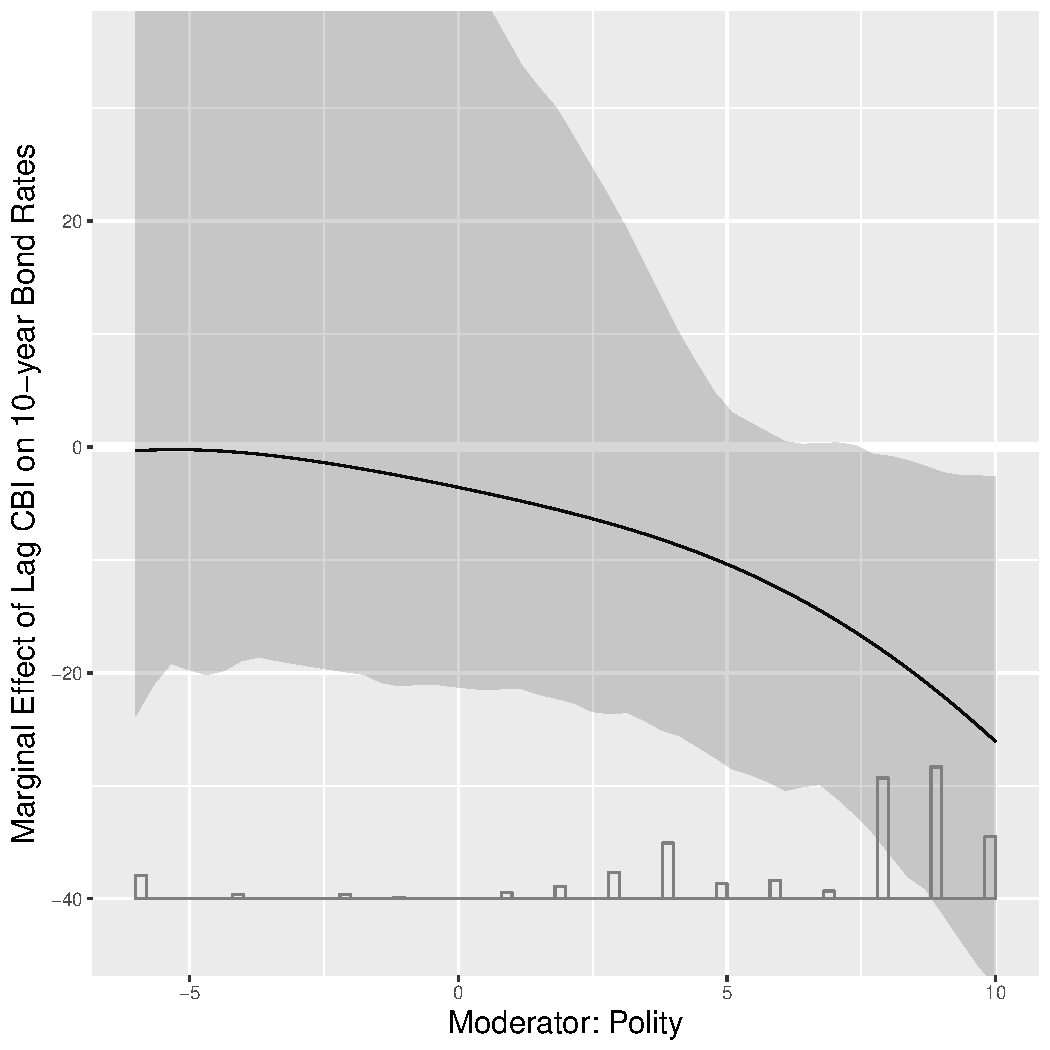
\includegraphics[width=0.45\textwidth]{bodea_2015b_smooth.pdf}}
\end{figure}%\vspace{-2em}
\clearpage



%%%%%%%%%%%%%%%%%%%%%%%%%%%%%%%% 

\subsection{\citet{Bodea2015_IO} IO} \label{bodea_IO}


First Interaction:


\paragraph{Claim on conditionality (Figure 2 in manuscript):} \emph{``Despite mixed empirical
  evidence, in the past two decades central bank independence (CBI) has
  been on the rise under the assumption that it ensures price
  stability. ... Empirical results are robust and support a discipline
  effect conditioned by political institutions, as well as a
  credibility effect.''} (Abstract)

\emph{``Figure 2 shows the marginal effect of CBI as POLITY and
  FREEDOM HOUSE democracy vary. The graphs confirm our expectations;
  the marginal effect of CBI is downward sloping but it is negative
  and statistically significant at high levels of democracy only
  (POLITY scores above 16). At low levels of POLITY, the marginal
  effect of CBI is positive but statistically
  insignificant. Similarly, the marginal effect of CBI is negative and
  significant only when the FREEDOM HOUSE score is greater than about  5.''} (p. 49)



\paragraph{Key variables for conditional relationship 1:} Outcome Y:
``M2 growth'' (\texttt{logdm2}); treatment D: ``central bank
independence'' (\texttt{CBI}); moderator X: ``Polity IV score'' (\texttt{polity2\_cen}).

\paragraph{Note:} The authors show 90\% confidence intervals in the paper, while in both the binning plot and the kernel smoothing plot, we use 95\% confidence intervals.


\clearpage


\begin{figure}[!ht]
  \caption{Results from \citet{Bodea2015_IO} }
  \setcounter{subfigure}{0}
  \centering
  \subfigure[Raw data]{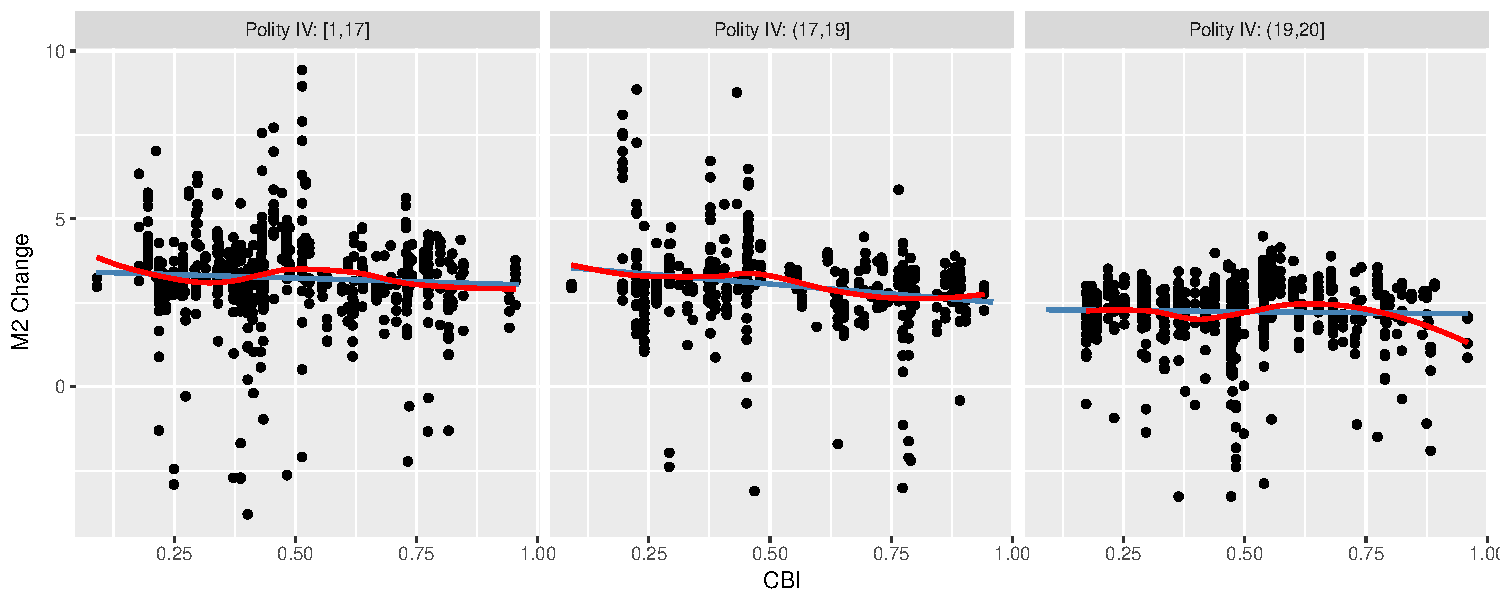
\includegraphics[width=1\textwidth]{bodea_io_2015a_raw.pdf} }
    \subfigure[GAM]{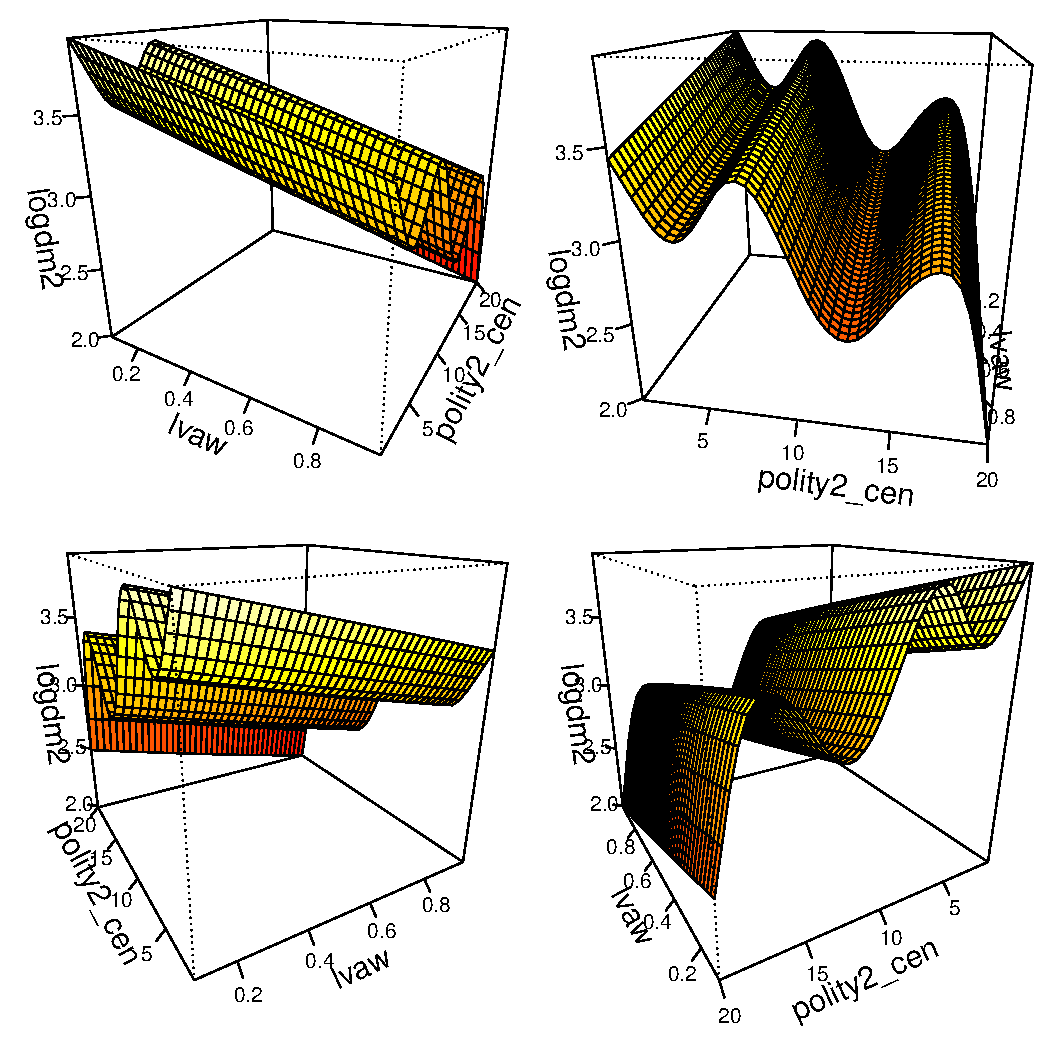
\includegraphics[width=0.45\textwidth]{bodea_io_2015a_gam.pdf}}\\
  \subfigure[Marginal Effects from Replicated Model (black line) and from Binning Estimator (white
dots)]{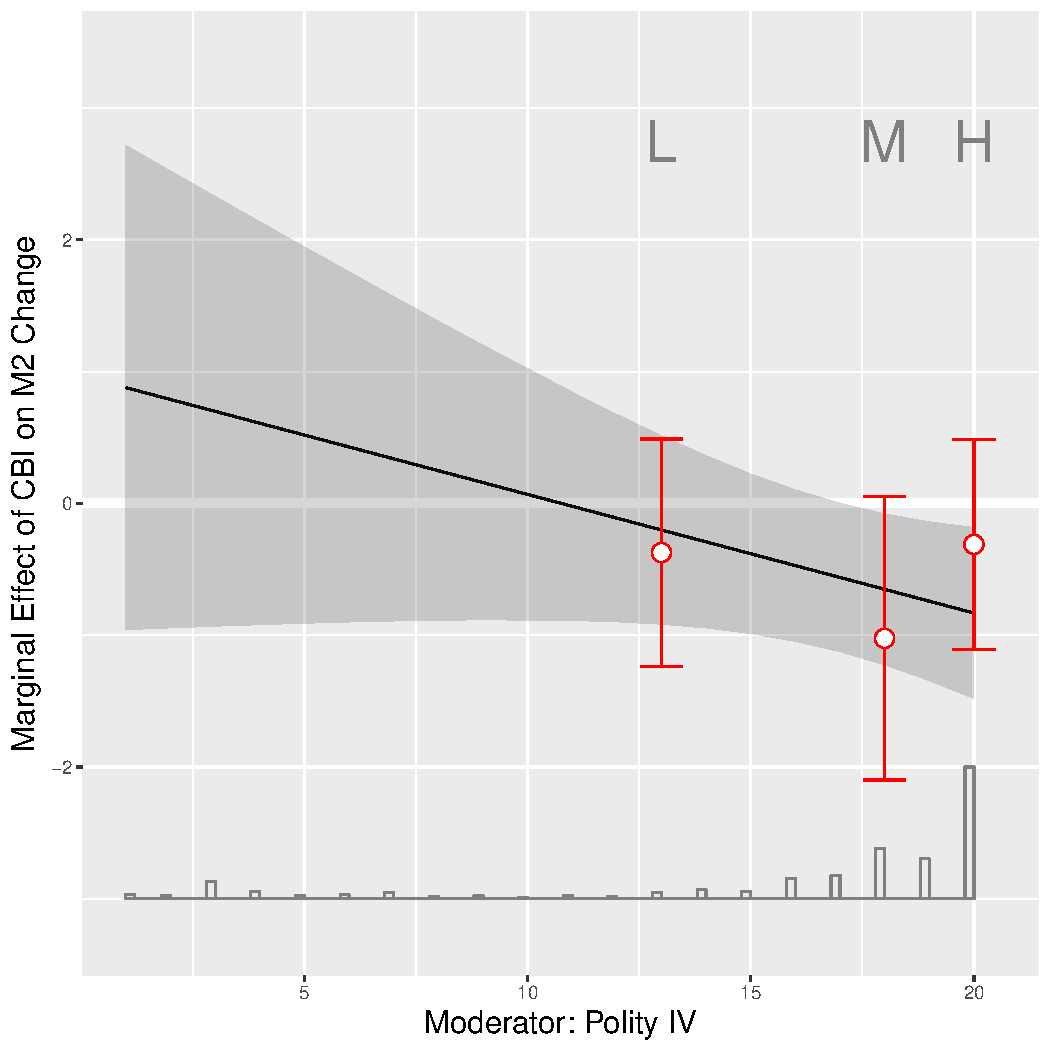
\includegraphics[width=0.45\textwidth]{bodea_io_2015a_est0.pdf}}
  \subfigure[Marginal Effects from Kernel Estimator]{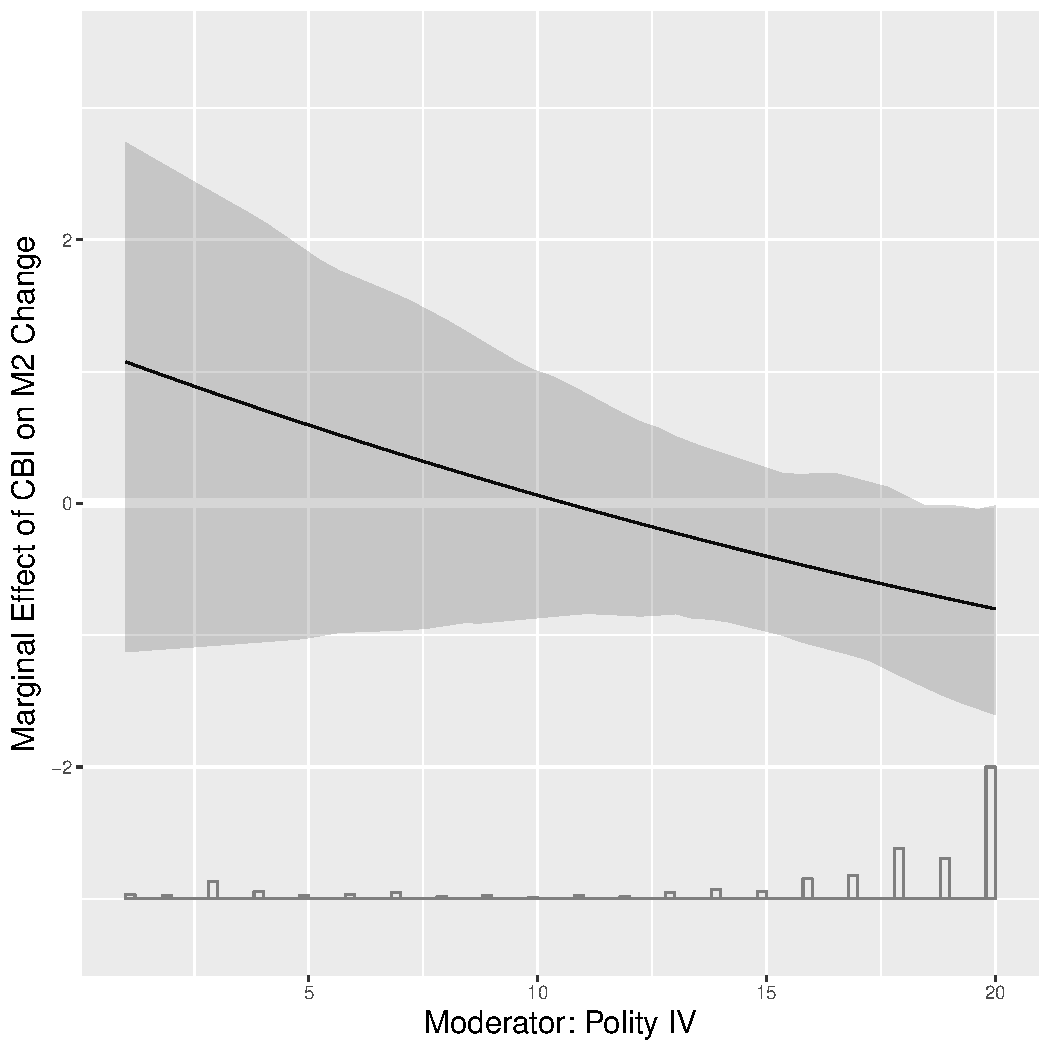
\includegraphics[width=0.45\textwidth]{bodea_io_2015a_smooth.pdf}}
\end{figure}%\vspace{-2em}


\clearpage

%%%% 

\noindent Second Interaction:

\paragraph{Claim on conditionality (Figure 2 in manuscript):}

\emph{``Figure 2 shows the marginal effect of CBI as POLITY and
  FREEDOM HOUSE democracy vary. The graphs confirm our expectations;
  the marginal effect of CBI is downward sloping but it is negative
  and statistically significant at high levels of democracy only
  (POLITY scores above 16). At low levels of POLITY, the marginal
  effect of CBI is positive but statistically
  insignificant. Similarly, the marginal effect of CBI is negative and
  significant only when the FREEDOM HOUSE score is greater than about  5.''} (p. 49)

\paragraph{Key variables for conditional relationship 2 :} Outcome Y:
``M2 growth'' (\texttt{logdm2}); treatment D: ``central bank
independence'' (\texttt{CBI}); moderator X: ``Freedom House democracy score'' (\texttt{FH\_trans}).


\paragraph{Note:} The authors show 90\% confidence intervals in the paper, while in both the binning plot and the kernel smoothing plot, we use 95\% confidence intervals.


\begin{figure}[!ht]
  \caption{Results from  \citet{Bodea2015_IO}}
  \setcounter{subfigure}{0}
  \centering
  \subfigure[Raw data]{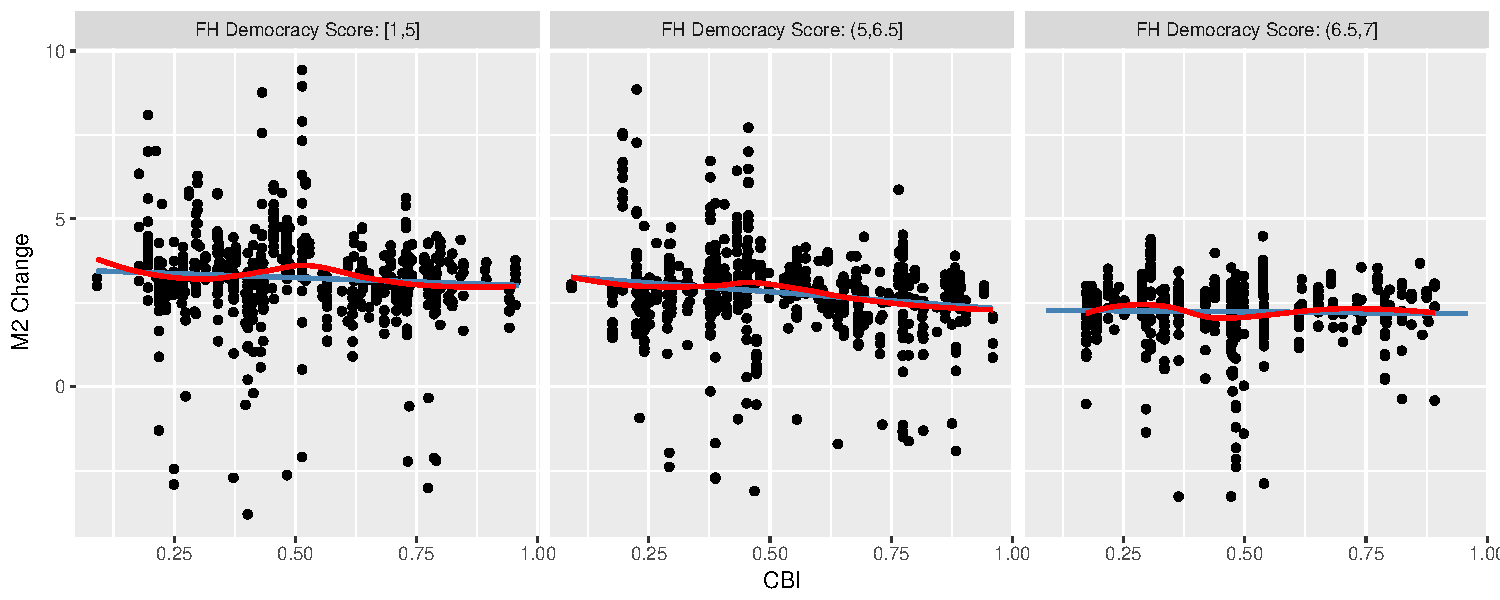
\includegraphics[width=1\textwidth]{bodea_io_2015b_raw.pdf} }
  \subfigure[GAM]{  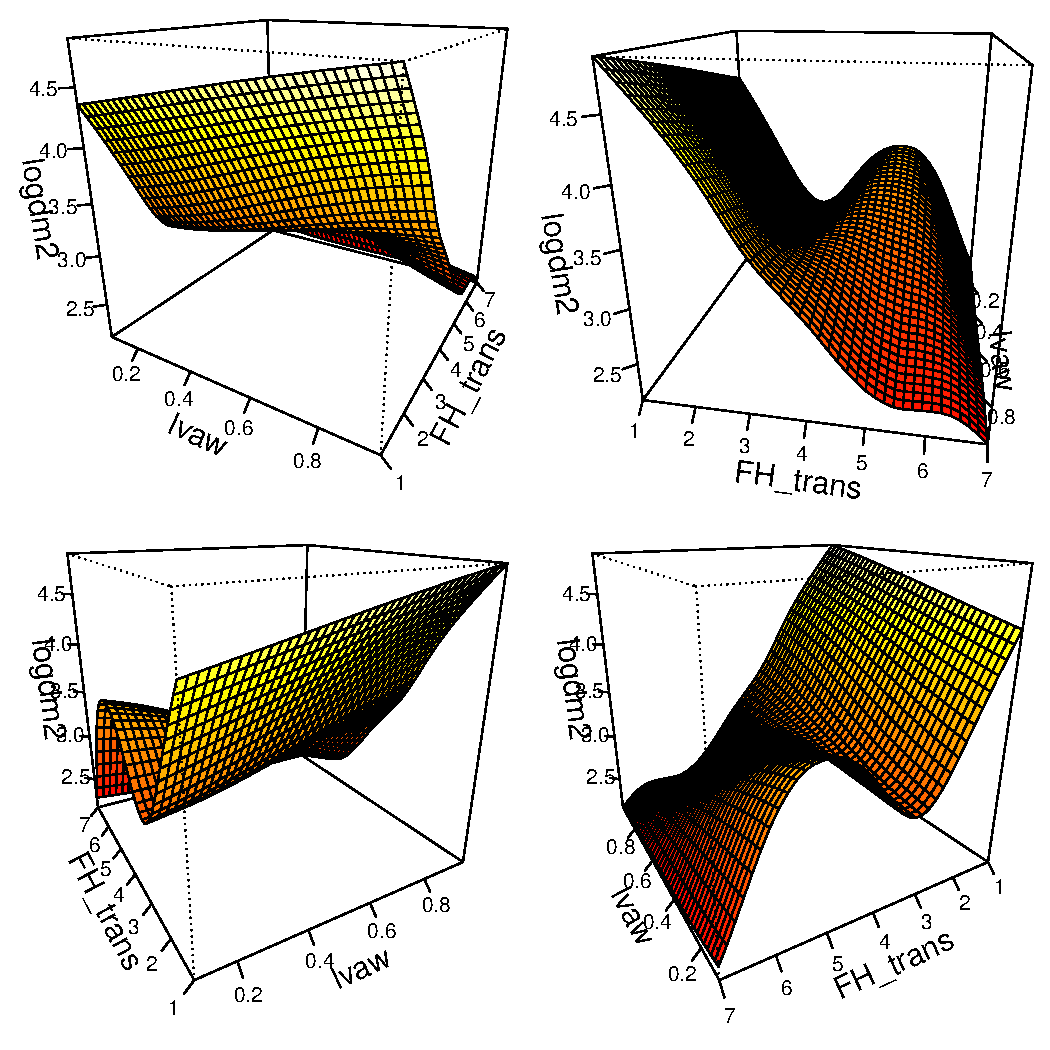
\includegraphics[width=0.45\textwidth]{bodea_io_2015b_gam.pdf}}\\
  \subfigure[Marginal Effects from Replicated Model (black line) and from Binning Estimator (white
dots)]{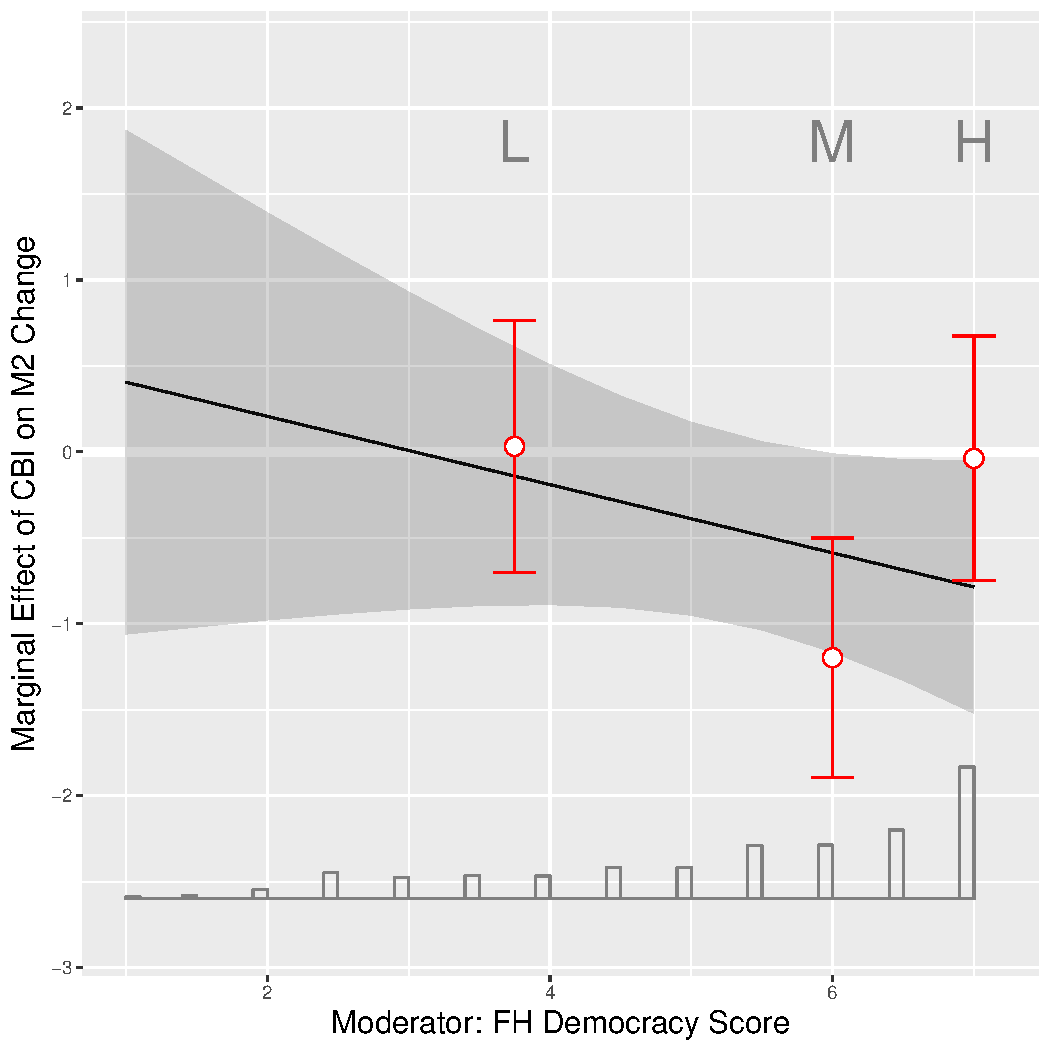
\includegraphics[width=0.45\textwidth]{bodea_io_2015b_est0.pdf}}
  \subfigure[Marginal Effects from Kernel Estimator]{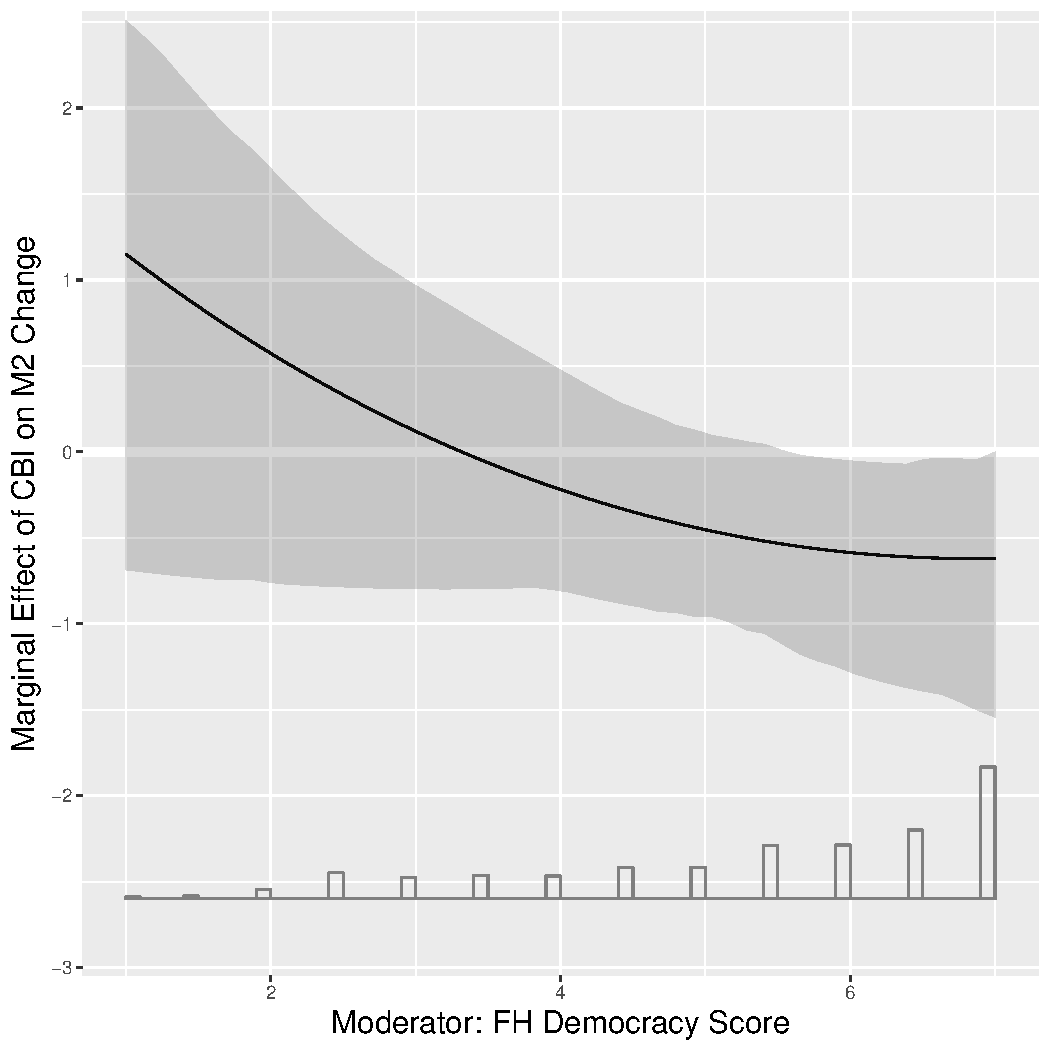
\includegraphics[width=0.45\textwidth]{bodea_io_2015b_smooth.pdf}}
\end{figure}%\vspace{-2em}
\clearpage

%%%% 
\noindent Third Interaction:

\paragraph{Claim on conditionality (Figure 4 in manuscript):}

\emph{``Figure 4 shows, however, that the marginal effect of CBI is
  significant only at high levels of Polity and FREEDOM HOUSE. The
  marginal effect line is downward sloping, suggesting that only for
  Polity scores greater than about 14 (FREEDOM HOUSE scores greater
  than about 4.5) does CBI significantly reduce inflation.''} (p. 52)

\paragraph{Key variables for conditional relationship:} Outcome Y:
``inflation'' (\texttt{lninfl}); treatment D: ``central bank
independence'' (\texttt{CBI}); moderator X: ``Polity IV score'' (\texttt{polity2\_cen}).

\paragraph{Note:} The authors show 90\% confidence intervals in the paper, while in both the binning plot and the kernel smoothing plot, we use 95\% confidence intervals.



\begin{figure}[!ht]
  \caption{Results from  \citet{Bodea2015_IO}}
  \setcounter{subfigure}{0}
  \centering
  \subfigure[Raw data]{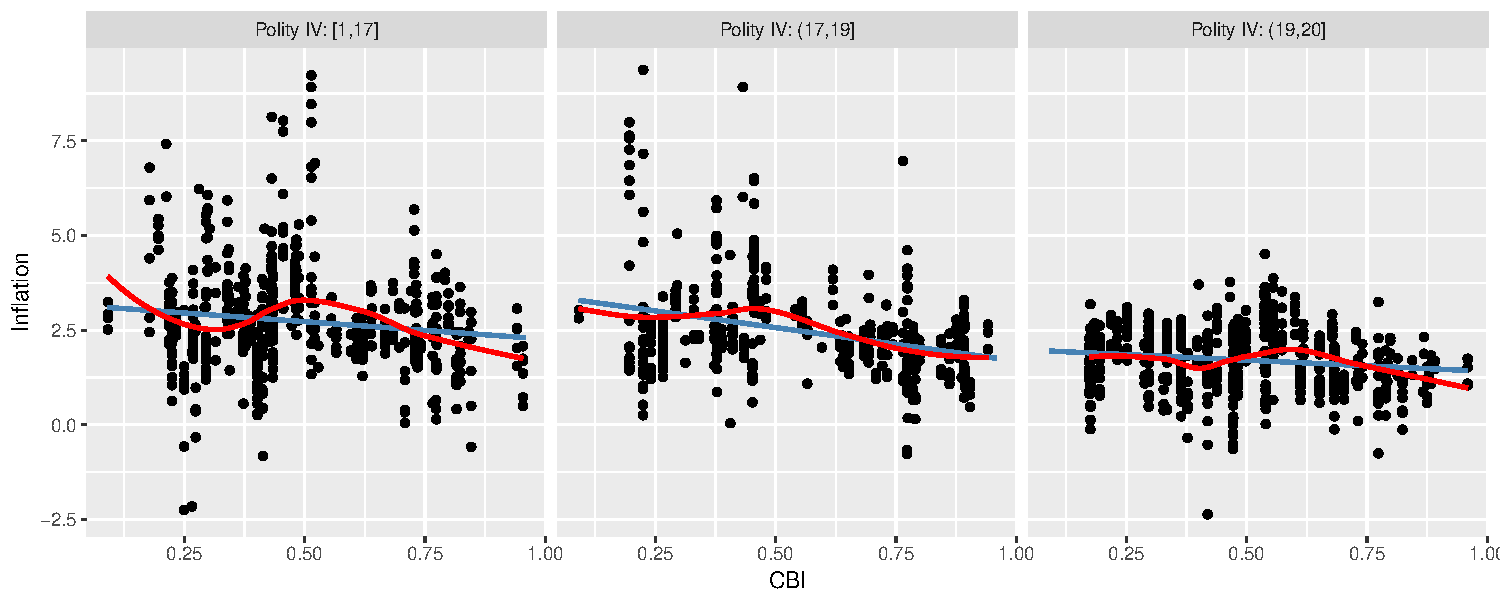
\includegraphics[width=1\textwidth]{bodea_io_2015c_raw.pdf} }
  \subfigure[GAM]{ 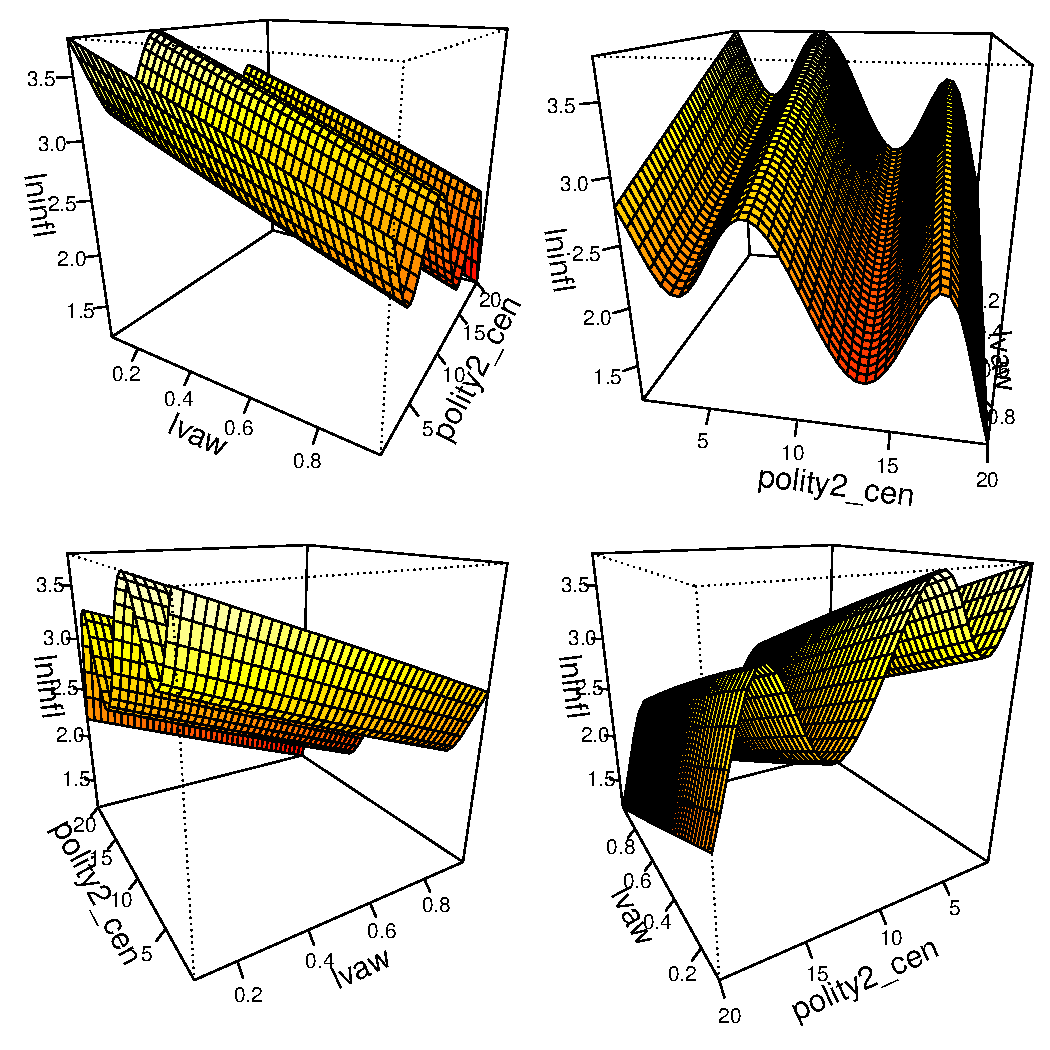
\includegraphics[width=0.45\textwidth]{bodea_io_2015c_gam.pdf}}\\
  \subfigure[Marginal Effects from Replicated Model (black line) and from Binning Estimator (white
dots)]{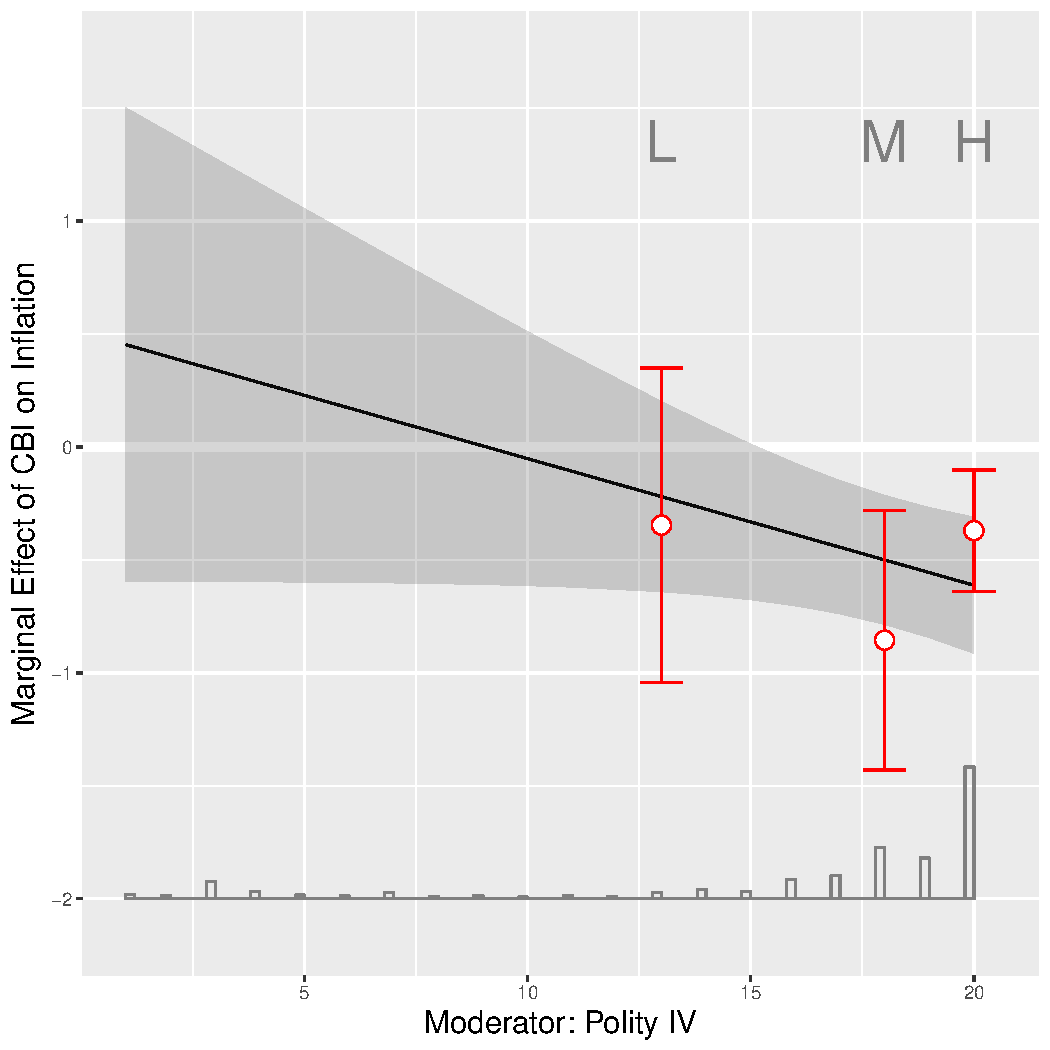
\includegraphics[width=0.45\textwidth]{bodea_io_2015c_est0.pdf}}
  \subfigure[Marginal Effects from Kernel Estimator]{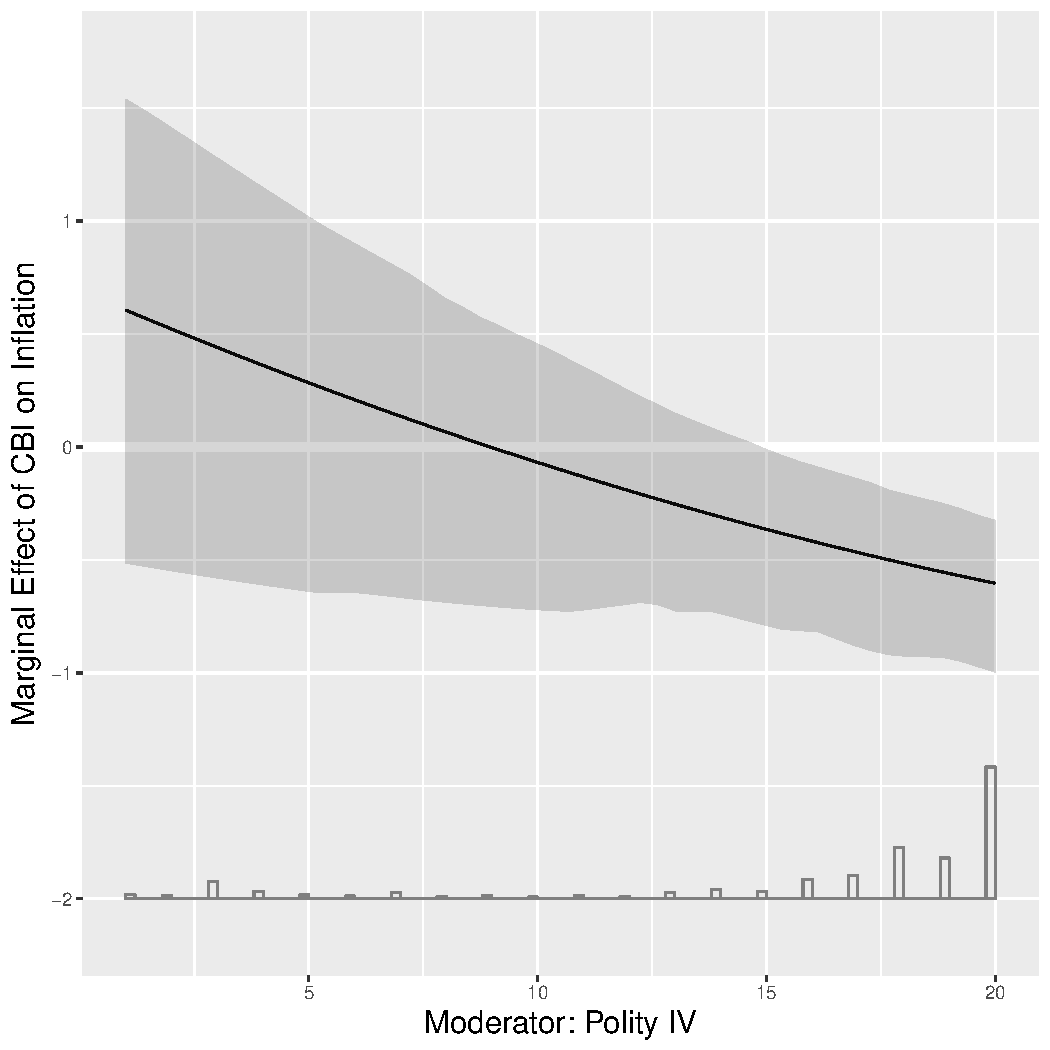
\includegraphics[width=0.45\textwidth]{bodea_io_2015c_smooth.pdf}}
\end{figure}%\vspace{-2em}

\clearpage
%%%% 
\noindent Fourth Interaction:

\paragraph{Claim on conditionality (Figure 4 in manuscript):}

\emph{``Figure 4 shows, however, that the marginal effect of CBI is
  significant only at high levels of Polity and FREEDOM HOUSE. The
  marginal effect line is downward sloping, suggesting that only for
  Polity scores greater than about 14 (FREEDOM HOUSE scores greater
  than about 4.5) does CBI significantly reduce inflation.''} (p. 52)

\paragraph{Key variables for conditional relationship:} Outcome Y:
``inflation'' (\texttt{lninfl}); treatment D: ``central bank
independence'' (\texttt{CBI}); moderator X:  ``Freedom
House democracy score'' (\texttt{FH\_trans}).

\paragraph{Note:} The authors show 90\% confidence intervals in the paper, while in both the binning plot and the kernel smoothing plot, we use 95\% confidence intervals.


\begin{figure}[!ht]
  \caption{Results from  \citet{Bodea2015_IO}}
  \setcounter{subfigure}{0}
  \centering
  \subfigure[Raw data]{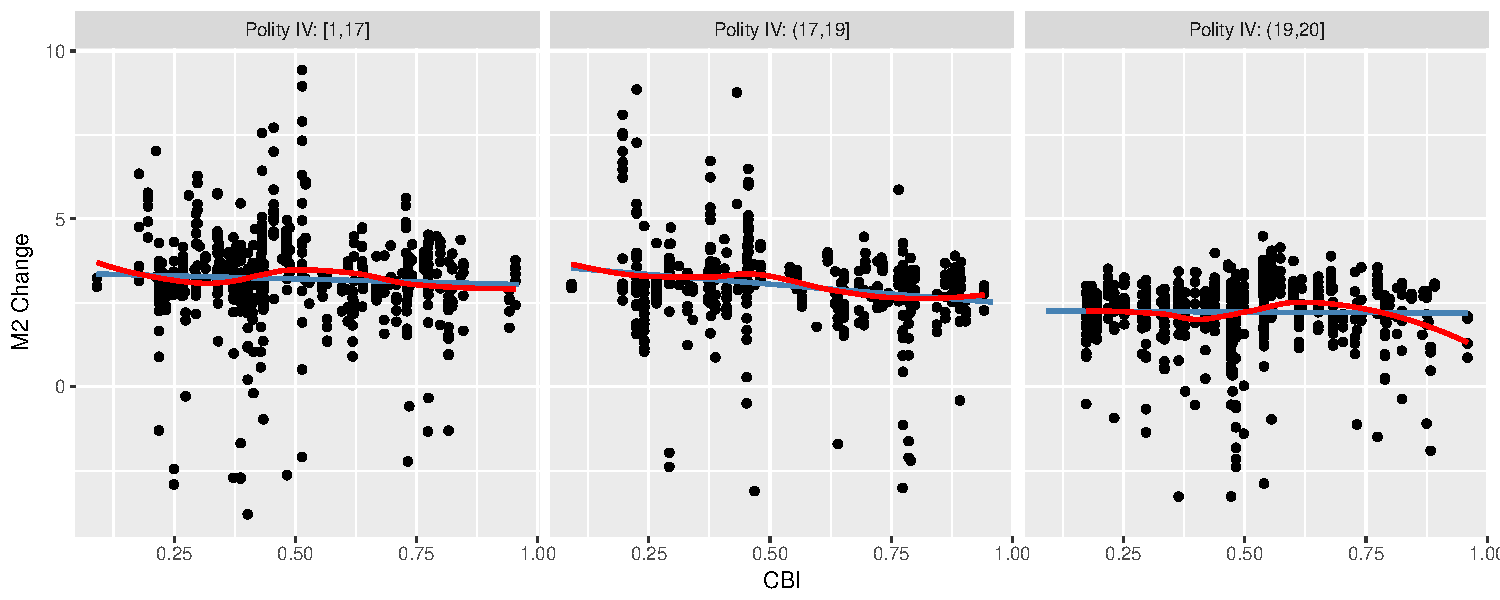
\includegraphics[width=1\textwidth]{bodea_io_2015d_raw.pdf} }
  \subfigure[GAM]{  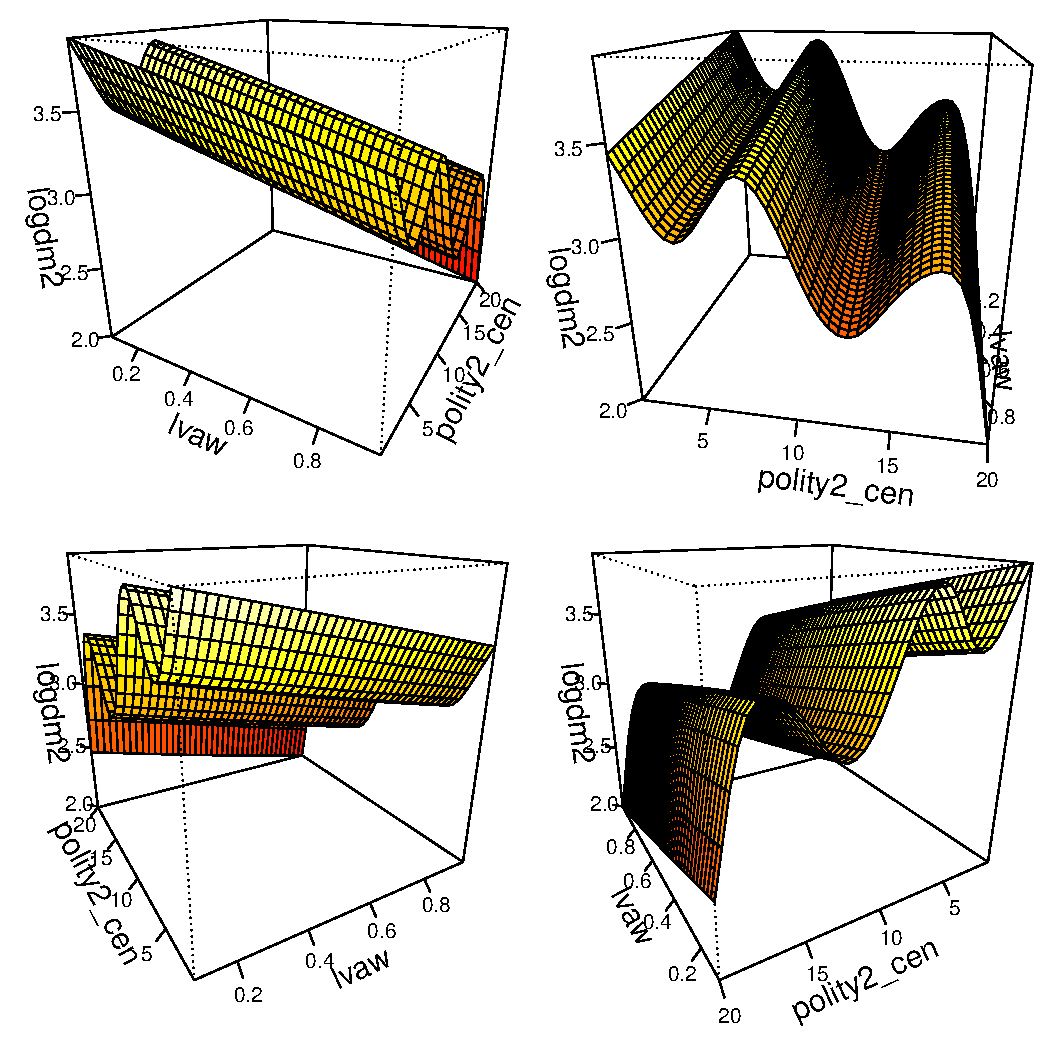
\includegraphics[width=0.4\textwidth]{bodea_io_2015d_gam.pdf}}\\
  \subfigure[Marginal Effects from Replicated Model (black line) and from Binning Estimator (white
dots)]{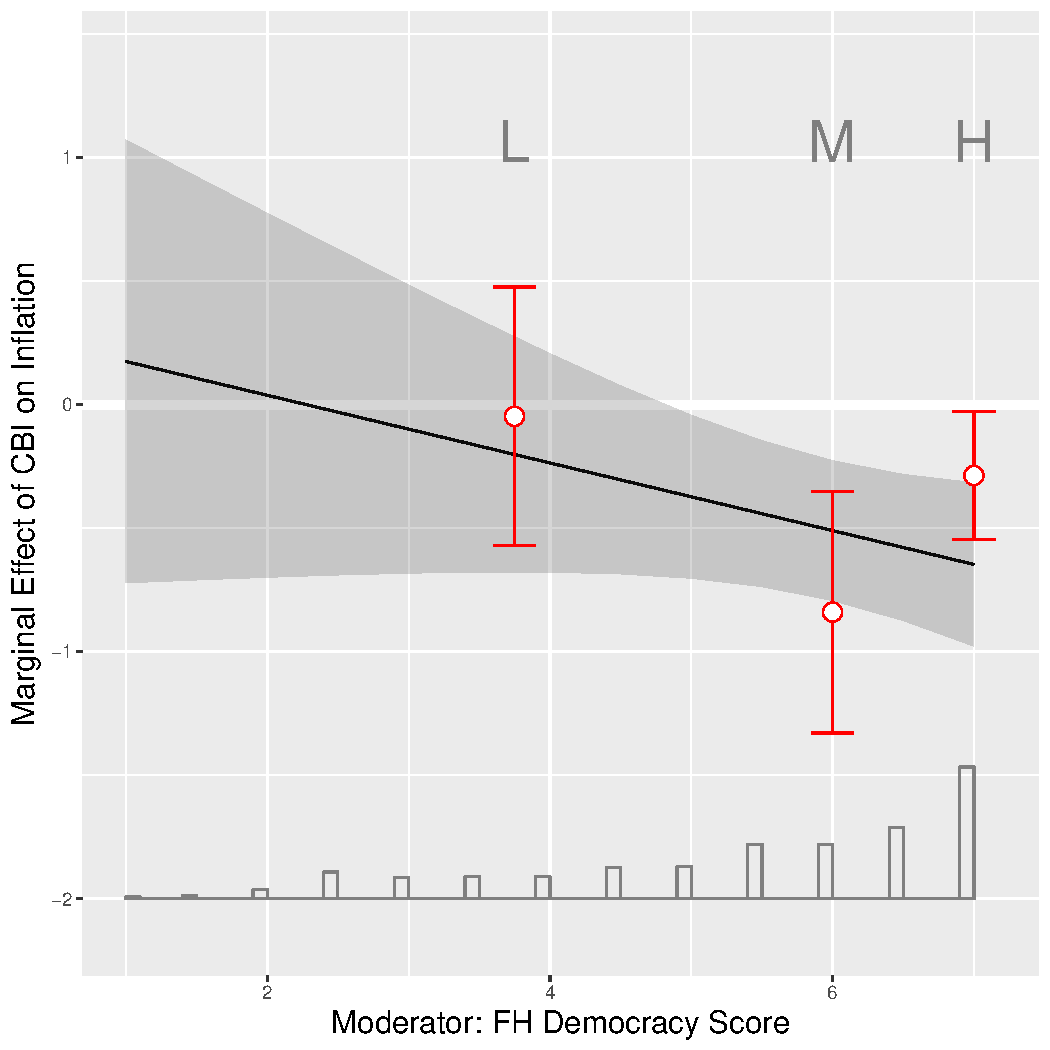
\includegraphics[width=0.45\textwidth]{bodea_io_2015d_est0.pdf}}
  \subfigure[Marginal Effects from Kernel Estimator]{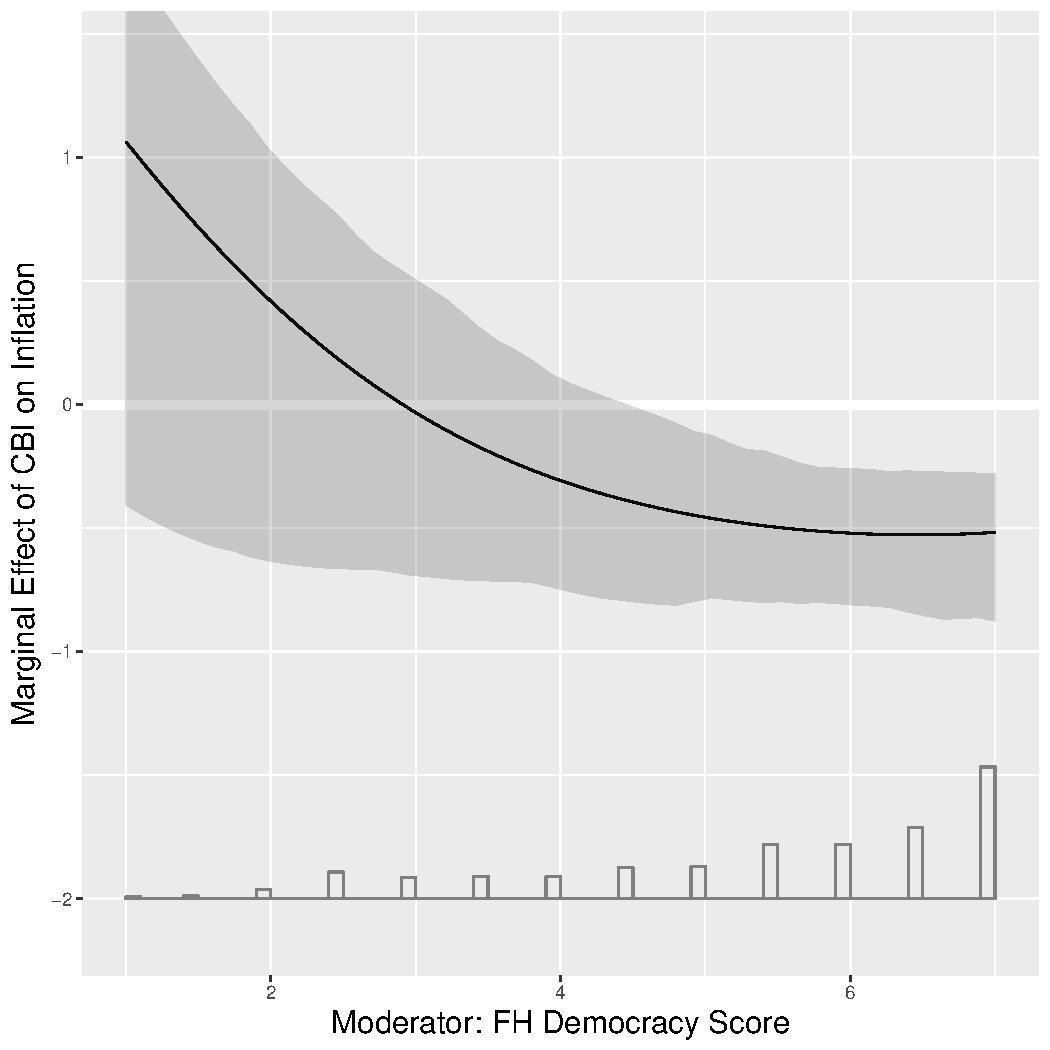
\includegraphics[width=0.45\textwidth]{bodea_io_2015d_smooth.pdf}}
\end{figure}%\vspace{-2em}
\clearpage





\subsection{\citet{Carpenter2014} APSR} \label{carpenter}

\paragraph{Claim on conditionality (Figure 4 in manuscript):} \emph{``[W]e note that
  women’s canvassing was far more efficacious when the prayer of the
  petition contained a protest against the gag rule. Figure 4 presents
  the marginal effect of the percentage of county petitions canvassed
  by women (in terms of additional signatures per 1,000 county
  population) as a function of the percentage of county petitions
  whose prayer focuses on the gag rule. ...The marginal-effects plot
  demonstrates that the effect of women’s canvassing is positive and
  statistically differentiable from zero for all values of the
  gag-rule focus variable.''} (pp. 490-91). 

\paragraph{Key variables for the conditional relationship:} Outcome Y:
``total names per 1000'' (\texttt{totnamesper1000}); treatment D: ``percent women's only petition''
(\texttt{pctpetwomen}); moderator X: ``percent focus gag rule'' (\texttt{pctfocgag}). 

\clearpage

\begin{figure}[!ht]
  \caption{Results from \citet{Carpenter2014} }
  \setcounter{subfigure}{0}
  \centering
  \subfigure[Raw data]{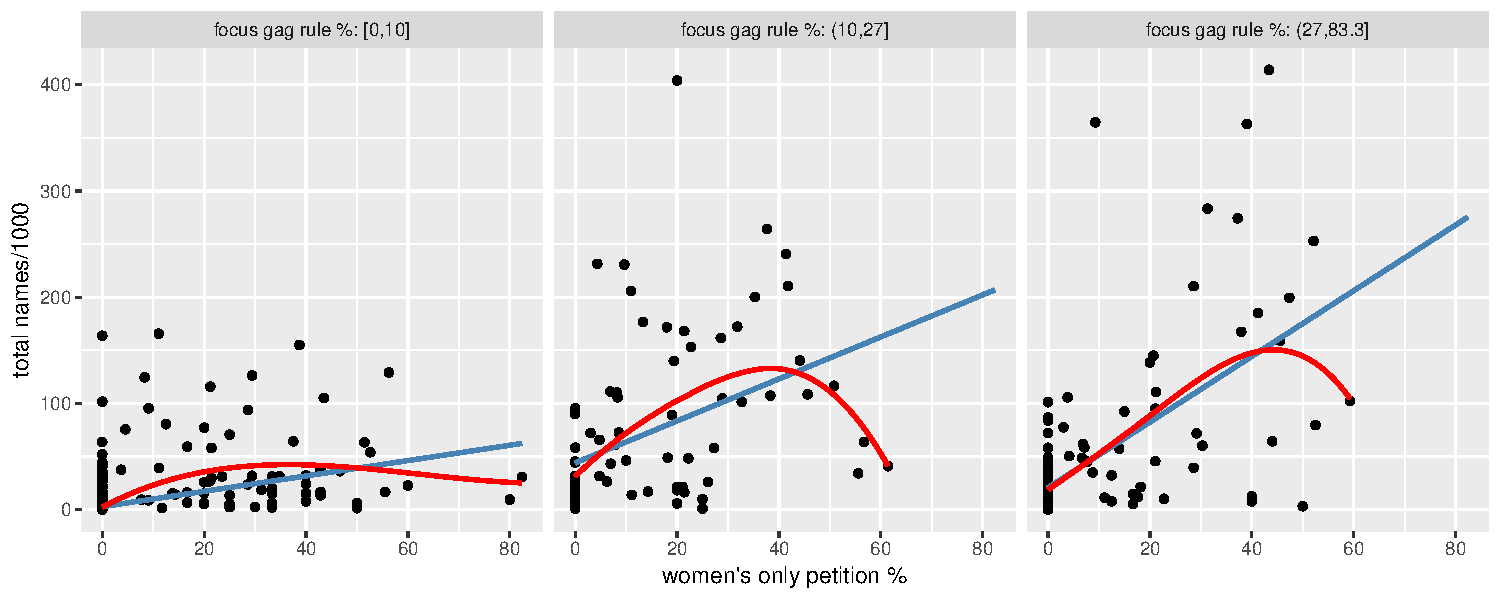
\includegraphics[width=0.8\textwidth]{carpenter_2014_raw.pdf} }
    \subfigure[GAM]{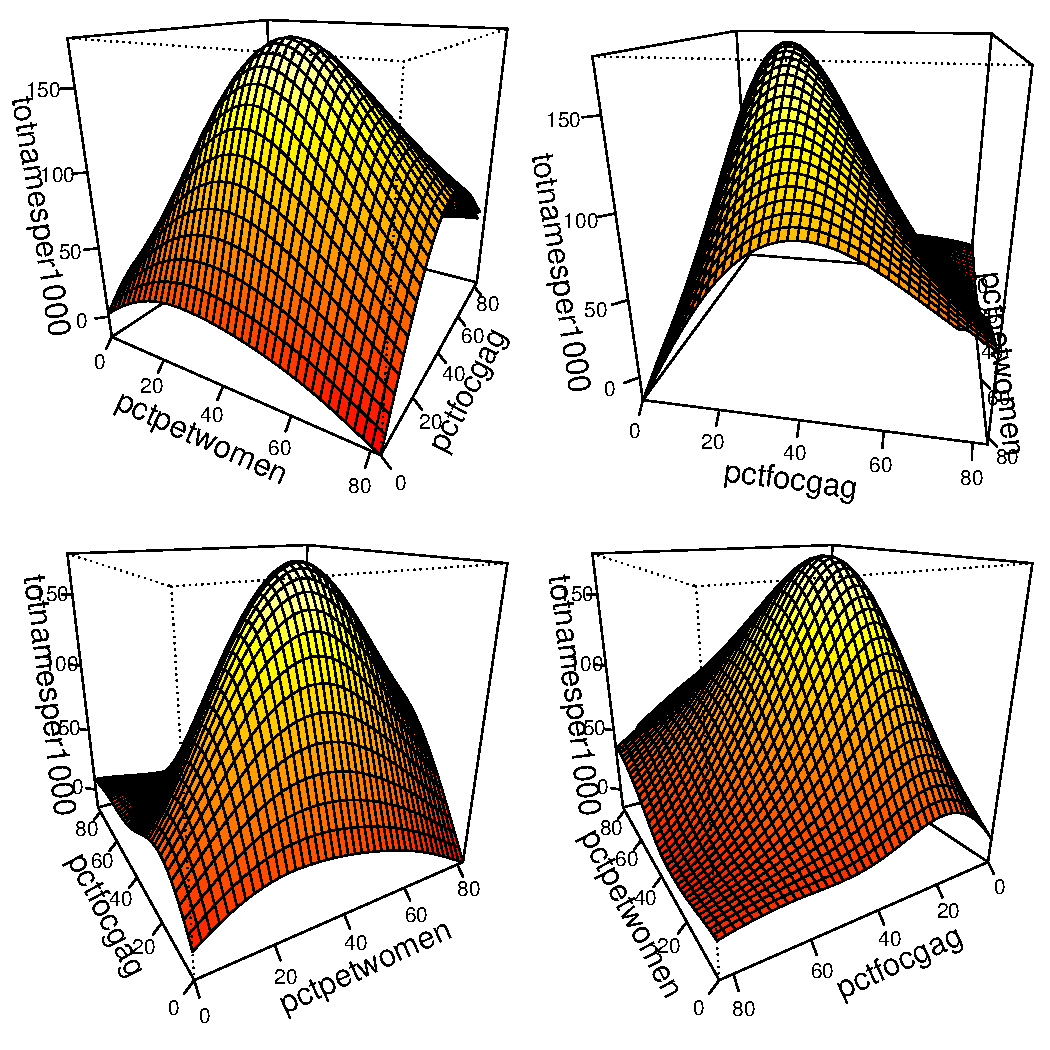
\includegraphics[width=.4\textwidth]{carpenter_2014_gam.pdf} }\\
  \subfigure[Marginal Effects from Replicated Model (black line) and from Binning Estimator (white
dots)]{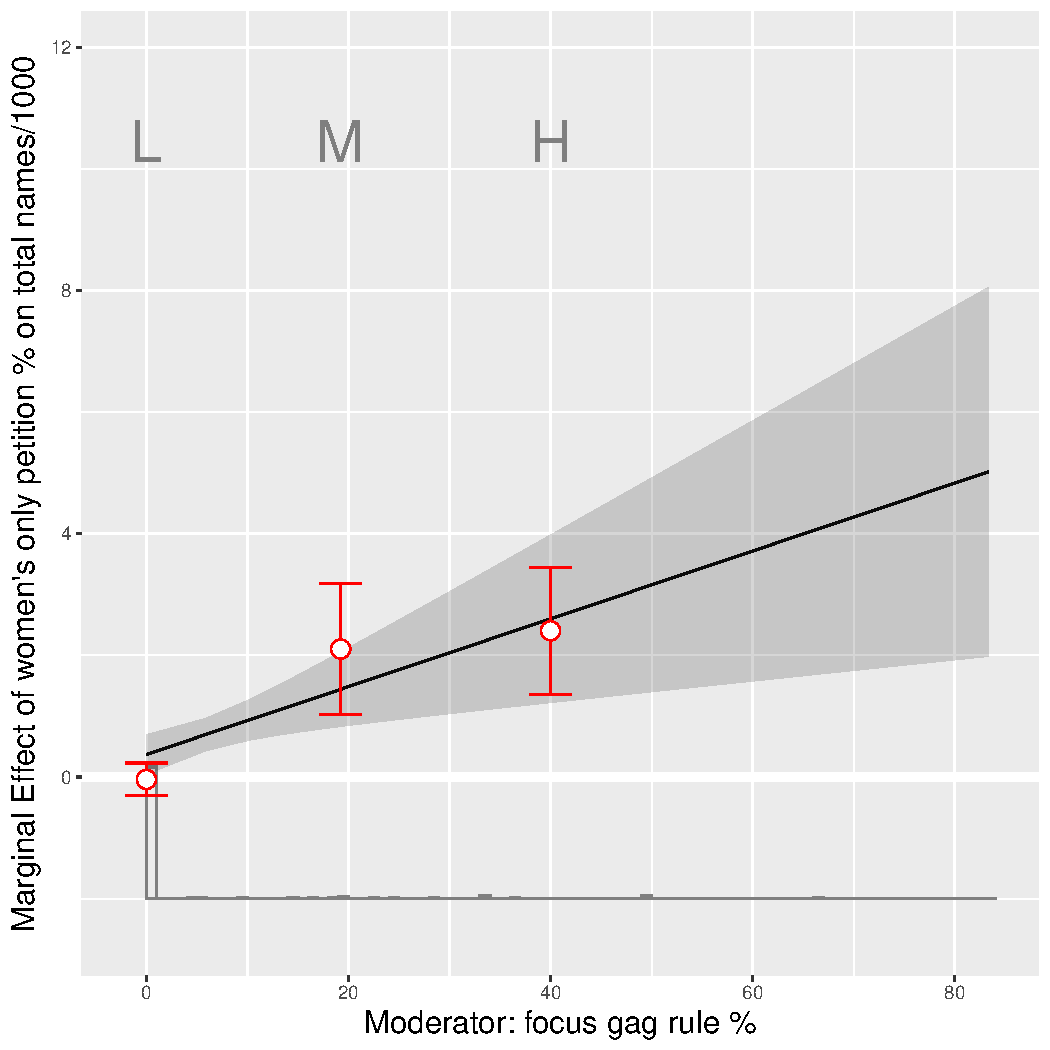
\includegraphics[width=0.45\textwidth]{carpenter_2014_est0.pdf}}
  \subfigure[Marginal Effects from Kernel Estimator]{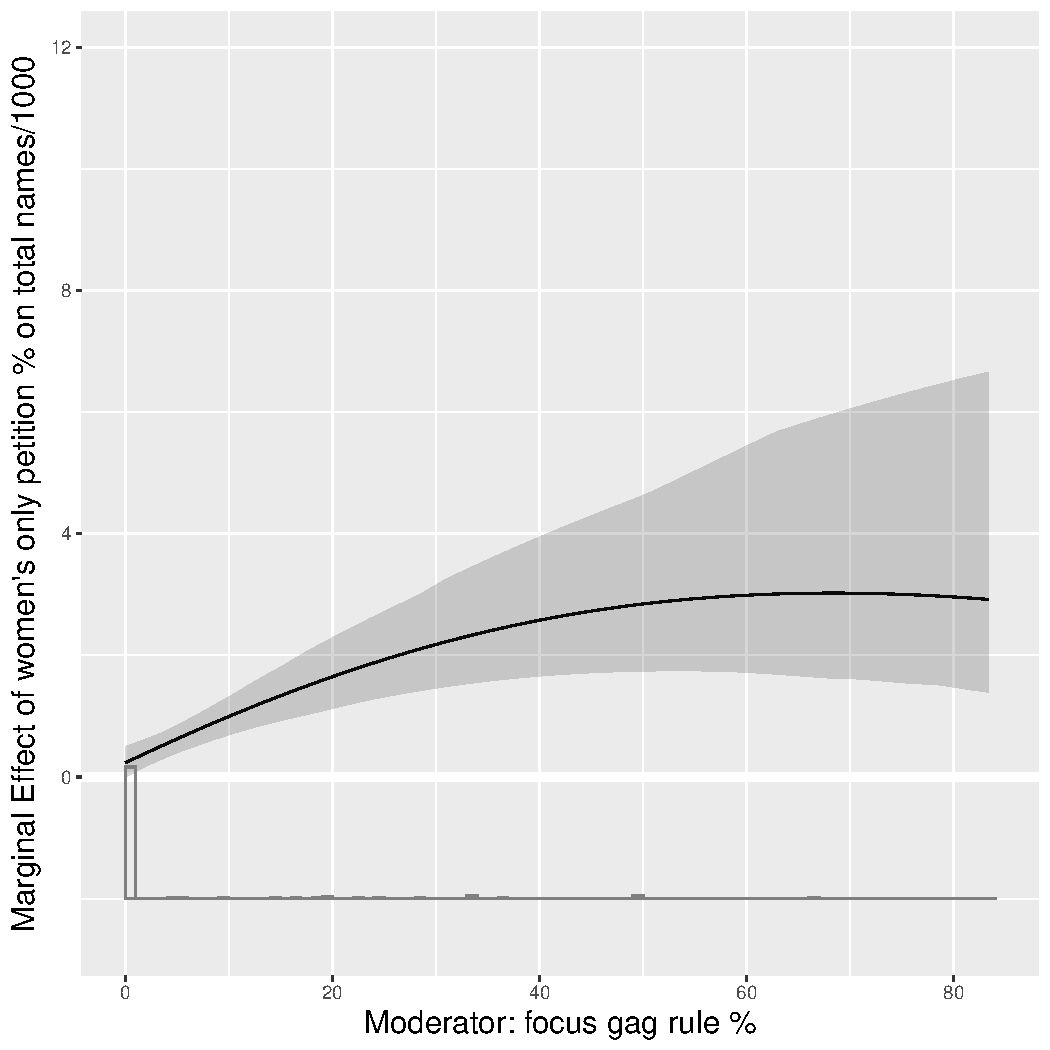
\includegraphics[width=0.45\textwidth]{carpenter_2014_smooth.pdf}}
\end{figure}
\clearpage


\subsection{\citet{chapman2009audience} IO} \label{chapman}

\paragraph{Claim on conditionality:} \emph{``This article
  tests this conditional relationship in the context of changes in
  presidential approval surrounding military disputes, using a measure
  of preference distance between the United States and veto-wielding
  members of the UN Security Council. Findings indicate that
  short-term changes in presidential approval surrounding the onset of
  military disputes in the United States between 1946 and 2001 have
  been significantly large when accompanied by a positive resolution
  for a Security Council that is more distant in terms of foreign
  policy preferences''} (Abstract). 

\emph{``Rallies with UN authorization are only larger than average
  when the pivotal member is ideologically distant from the United
  States... Clearly, the effect of authorization on rallies decreases
  as similarity increases: foreign policy actions that receive
  authorization from a less conservative institution receive similar
  rallies to those that do not receive authorization from an IO''}
(p. 756)

\paragraph{Key variables for the conditional relationship:} Outcome Y:
``rallies'' (\texttt{rally}); treatment D: ``UN authorization''
(\texttt{unauth}); moderator X: ``US affinity with UN Security Council
'' (\texttt{S}).

\paragraph{Note:}  Among 196 observations, there are only 6 positive cases
(\texttt{unauth=1}). 

\bigskip
\newpage



\begin{figure}[!ht]
  \caption{Results from \citet{chapman2009audience}}
  \setcounter{subfigure}{0}
  \centering
  \subfigure[Raw data]  { 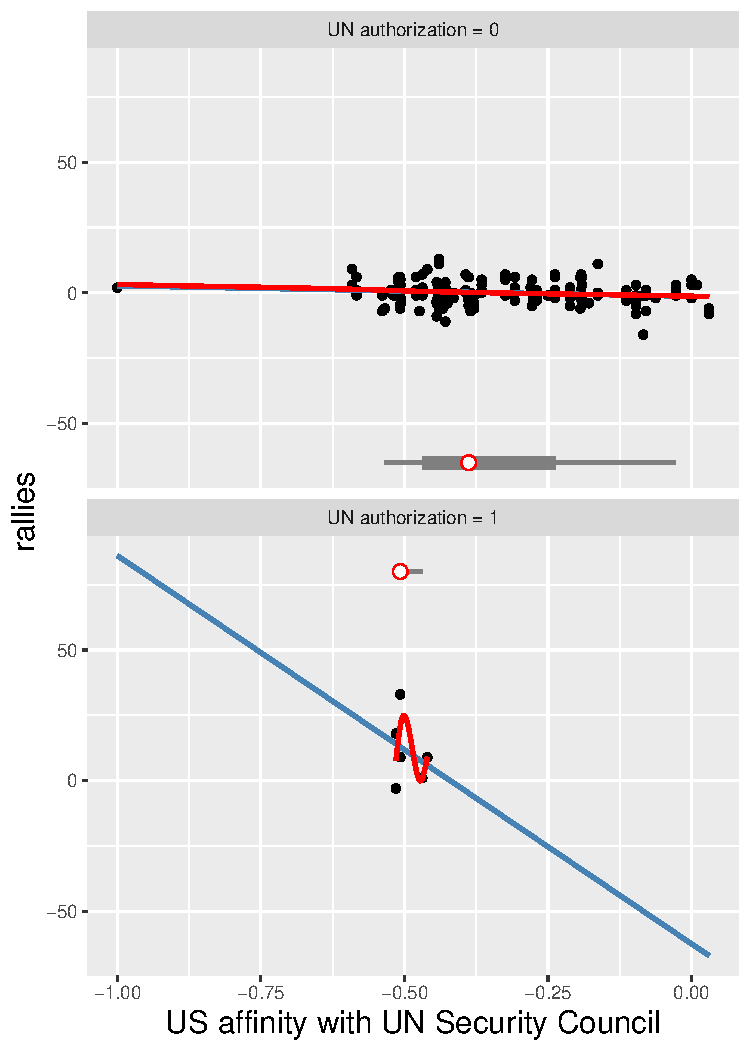
\includegraphics[width=0.5\textwidth]{chapman_2009_raw.pdf}}\\
  \subfigure[Marginal Effects from Replicated Model (black line) and from Binning Estimator (white
dots)]{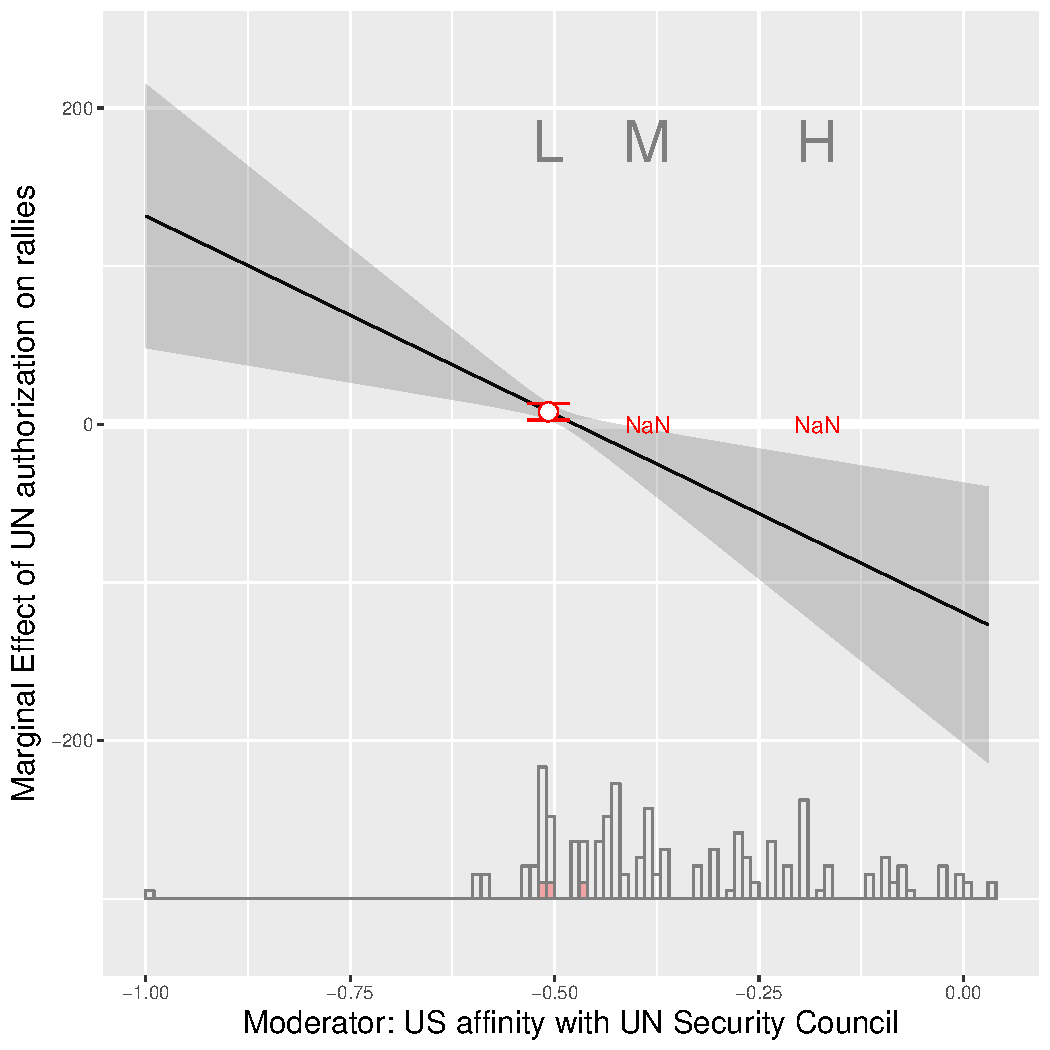
\includegraphics[width=0.48\textwidth]{chapman_2009_est0.pdf}}
  \subfigure[Marginal Effects from Kernel Estimator]{\includegraphics[width=0.48\textwidth]{chapman_2009_smooth.pdf}}
\end{figure}
\clearpage



\subsection{\citet{clark2006rehabilitating} CPS} \label{clark}


\noindent First Interaction:


\paragraph{Claims on conditionality (Figure 1 in manuscript):} \emph{``All three
  figures (in Figure 1) clearly illustrate that in established democracies, ethnic
  heterogeneity significantly increases the number of parties once the
  electoral system is sufficiently permissive. This is exactly what
  Duverger's theory predicts''} (p. 700).


\paragraph{Key variables for the first conditional relationship:} Outcome Y:
``effective number of parties'' 
(\texttt{enepl}); treatment D:  ``ethnic
heterogeneity'' (\texttt{eneg}); moderator X: ``log average district magnitude'' (\texttt{logmag}). 

\paragraph{Note:} The authors show 90\% confidence intervals in the paper, while in both the binning plot and the kernel smoothing plot, we use 95\% confidence intervals.

\clearpage



\begin{figure}[!ht]
  \caption{Results from \citet{clark2006rehabilitating} }
  \setcounter{subfigure}{0}
  \centering
  \subfigure[Raw data]{\includegraphics[width=1\textwidth]{clark_2006a_raw.pdf} }
  \subfigure[GAM]{\includegraphics[width=0.45\textwidth]{clark_2006a_gam.pdf}}\\
  \subfigure[Marginal Effects from Replicated Model (black line) and from Binning Estimator (white
dots)]{\includegraphics[width=0.45\textwidth]{clark_2006a_est0.pdf}}
  \subfigure[Marginal Effects from Kernel Estimator]{\includegraphics[width=0.45\textwidth]{clark_2006a_smooth.pdf}}
\end{figure}%\vspace{-2em}


\clearpage

\noindent Second Interaction:


\paragraph{Claims on conditionality (Figure 1 in manuscript, middle panel):} \emph{``All three
  figures (in Figure 1) clearly illustrate that in established democracies, ethnic
  heterogeneity significantly increases the number of parties once the
  electoral system is sufficiently permissive. This is exactly what
  Duverger’s theory predicts''} (p. 700).

\paragraph{Key variables for the first conditional relationship:} Outcome Y:
``effective number of parties'' 
(\texttt{enpv}); treatment D:  ``ethnic
heterogeneity'' (\texttt{eneth}); moderator X: ``log average district magnitude'' (\texttt{lnml}). 

\paragraph{Note:} The authors show 90\% confidence intervals in the paper, while in both the binning plot and the kernel smoothing plot, we use 95\% confidence intervals.

\begin{figure}[!ht]
  \caption{Results from \citet{clark2006rehabilitating} }
  \setcounter{subfigure}{0}
  \centering
  \subfigure[Raw data]{\includegraphics[width=1\textwidth]{clark_2006b_raw.pdf} }
  \subfigure[GAM]{\includegraphics[width=0.45\textwidth]{clark_2006b_gam.pdf}}\\
  \subfigure[Marginal Effects from Replicated Model (black line) and from Binning Estimator (white
dots)]{\includegraphics[width=0.45\textwidth]{clark_2006b_est0.pdf}}
  \subfigure[Marginal Effects from Kernel Estimator]{\includegraphics[width=0.45\textwidth]{clark_2006b_smooth.pdf}}
\end{figure}%\vspace{-2em}
\clearpage



\noindent Third Interaction:

\paragraph{Claims on conditionality (Figure 1 in manuscript, bottom panel):} \emph{``All three
  figures (in Figure 1) clearly illustrate that in established democracies, ethnic
  heterogeneity significantly increases the number of parties once the
  electoral system is sufficiently permissive. This is exactly what
  Duverger’s theory predicts''} (p.\ 700).


\paragraph{Key variables for the first conditional relationship:} Outcome Y:
``effective number of parties'' 
(\texttt{enep1}); treatment D:  ``ethnic
heterogeneity'' (\texttt{eneg}); moderator X: ``log average district magnitude'' (\texttt{logmag}). 

\paragraph{Note:} The authors show 90\% confidence intervals in the paper, while in both the binning plot and the kernel smoothing plot, we use 95\% confidence intervals.


\begin{figure}[!ht]
  \caption{Results from \citet{clark2006rehabilitating} }
  \setcounter{subfigure}{0}
  \centering
  \subfigure[Raw data]{ \centering\includegraphics[width=1\textwidth]{clark_2006c_raw.pdf} }
  \subfigure[GAM]{\includegraphics[width=0.45\textwidth]{clark_2006c_gam.pdf}}\\
  \subfigure[Marginal Effects from Replicated Model (black line) and from Binning Estimator (white
dots)]{\includegraphics[width=0.45\textwidth]{clark_2006c_est0.pdf}}
  \subfigure[Marginal Effects from Kernel Estimator]{\includegraphics[width=0.45\textwidth]{clark_2006c_smooth.pdf}}
\end{figure}%\vspace{-2em}

\clearpage

\noindent Fourth Interaction:


\paragraph{Claims on conditionality (Figure 2 in manuscript):} \emph{``Figure 2 plots the marginal effect of temporally proximate
  presidential elections. \ldots It should be clear that temporally
  proximate presidential elections have a strong reductive effect on
  the number of parties when there are few presidential candidates''} (p. 702).

\paragraph{Key variables for the second conditional relationship:} Outcome Y:
``effective number of parties'' (\texttt{enepl}); treatment D:  ``proximate presidential elections'' (\texttt{proximityl}); moderator X: ``effective number of pres. candidates'' (\texttt{enpres}). 

\paragraph{Note:} The authors show 90\% confidence intervals in the paper, while in both the binning plot and the kernel smoothing plot, we use 95\% confidence intervals.


\begin{figure}[!ht]
  \caption{Results from \citet{clark2006rehabilitating} }
  \setcounter{subfigure}{0}
  \centering
  \subfigure[Raw data]{\includegraphics[width=1\textwidth]{clark_2006d_raw.pdf} }
  \subfigure[GAM]{\includegraphics[width=0.45\textwidth]{clark_2006d_gam.pdf}}\\
  \subfigure[Marginal Effects from Replicated Model (black line) and from Binning Estimator (white
dots)]{\includegraphics[width=0.45\textwidth]{clark_2006d_est0.pdf}}
  \subfigure[Marginal Effects from Kernel Estimator]{\includegraphics[width=0.45\textwidth]{clark_2006d_smooth.pdf}}
\end{figure}%\vspace{-2em}


\clearpage




\subsection{\citet{Clark_2014} CPS} \label{clark2}

\paragraph{Claim on conditionality (Figure 2 in manuscript):} \emph{``We perform
  empirical analyses \ldots and test the hypothesis that when parties are
  more ideologically proximate to the mean voter position,
  character-based valence attributes will be of greater significance
  in determining parties' electoral fortunes. Surprisingly, we find no
  support for this hypothesis. Instead, our analyses suggest that the more ideologically dispersed parties are, the more likely it is that character-based valence attributes will affect parties' vote shares."} (Abstract). 

\emph{``This relationship indicates that, as parties become more
  dispersed on the left-right spectrum, voters weigh changes in
  parties' character-based valence attributes more heavily in their
  voting decisions."} (p.\ 185).

\paragraph{Key variables for the conditional relationship:} Outcome Y:
``change in vote share'' (\texttt{res\_votechgtt1}); treatment D:
``change in valence''
(\texttt{cgscn2tt1}); moderator X: ``change in party dispersion'' (\texttt{partydispuw}). 

\paragraph{Note:}  The dashed vertical line indicates the truncated interval of the moderator shown in the original marginal effect plot.


\begin{figure}[!ht]
  \caption{Results from   \citet{Clark_2014} }
  \setcounter{subfigure}{0}
  \centering
  \subfigure[Raw data] {\includegraphics[width=1\textwidth]{clark_2014_raw.pdf} }
  \subfigure[GAM]{ \includegraphics[width=0.45\textwidth]{clark_2014_gam.pdf}}\\
  \subfigure[Marginal Effects from Replicated Model (black line) and from Binning Estimator (white
dots)]{\includegraphics[width=0.45\textwidth]{clark_2014_est0.pdf}}
  \subfigure[Marginal Effects from Kernel Estimator]{\includegraphics[width=0.45\textwidth]{clark_2014_smooth.pdf}}
\end{figure}%\vspace{-2em}
\clearpage



\subsection{\citet{Hellwig2007} CPS} \label{hellwig}

\noindent First Interaction:

\paragraph{Claims on conditionality (Figure 1 in manuscript):} \emph{``Results support a
  government constraint hypothesis: Exposure to the world economy
  weakens connections between economic performance and support for
  political incumbents''} (Abstract).

\emph{``Figure 1 shows that trade openness reduces the positive
  relationship between economic performance and vote share for the
  incumbent.''} (p. 294).

\paragraph{Key variables for the conditional relationships:} Outcome Y:
``election'' (\texttt{incvotet}); treatment D: ``economy''
(\texttt{dgdp}); moderator X: ``trade as share of GDP '' 
(\texttt{tradeshr}, in Figure 1). 

\paragraph{Note:}  The dashed vertical line indicates the truncated interval of the moderator shown in the original marginal effect plot.



\begin{figure}[!ht]
  \caption{Results from \citet{Hellwig2007} }
  \setcounter{subfigure}{0}
  \centering
  \subfigure[Raw data]{\includegraphics[width=1\textwidth]{hellwig_2007a_raw.pdf} }
  \subfigure[GAM]{\includegraphics[width=0.45\textwidth]{hellwig_2007a_gam.pdf}}\\
  \subfigure[Marginal Effects from Replicated Model (black line) and from Binning Estimator (white
dots)]{\includegraphics[width=0.45\textwidth]{hellwig_2007a_est0.pdf}}
  \subfigure[Marginal Effects from Kernel Estimator]{\includegraphics[width=0.45\textwidth]{hellwig_2007a_smooth.pdf}}
\end{figure}
\clearpage



\noindent Second Interaction:

\paragraph{Claims on conditionality (Figure 2 in manuscript):}
\emph{``Figure 2 shows that the exposure to international capital flows also reduces the relationship between economic performance and election outcomes''} (p. 294).

\paragraph{Key variables for the conditional relationships:} Outcome Y:
``election'' (\texttt{incvotet}); treatment D: ``economy''
(\texttt{dgdp}); moderator X:  ``capital flows as share of GDP'' (\texttt{grosscap}) . 

\paragraph{Note:}  The dashed vertical line indicates the truncated interval of the moderator shown in the original marginal effect plot.


\begin{figure}[!ht]
  \caption{Results from \citet{Hellwig2007} }
  \setcounter{subfigure}{0}
  \centering
  \subfigure[Raw data]{g\includegraphics[width=1\textwidth]{hellwig_2007b_raw.pdf}}
  \subfigure[GAM]{ \includegraphics[width=0.45\textwidth]{hellwig_2007b_gam.pdf}}\\
  \subfigure[Marginal Effects from Replicated Model (black line) and from Binning Estimator (white
dots)]{\includegraphics[width=0.45\textwidth]{hellwig_2007b_est0.pdf}}
  \subfigure[Marginal Effects from Kernel Estimator]{\includegraphics[width=0.45\textwidth]{hellwig_2007b_smooth.pdf}}
\end{figure}
\clearpage





\subsection{\citet{Hicken2008} AJPS} \label{hicken}


\paragraph{Claim on conditionality (Figure 1, top left panel in manuscript):} \emph{``We find that
  though personal vote systems spend just as much on education as
  party vote systems, particularism in personal vote systems dampens
  the marginal effect of increased education spending on illiteracy
  and at its highest levels, incentives to cultivate a personal vote
  completely undermine the positive effects of increased education
  spending on literacy''} (Abstract).

\paragraph{Key variables for the conditional relationship:} Outcome Y:
``log illiteracy'' (\texttt{log\_illit\_all}); treatment D: ``education spending''
(\texttt{educgdp}); moderator X: ``parindex'' (\texttt{parindex}),
which is the average of three institutional variables: ``Ballot'',
``Pool'', and ``Vote''. We also use the three variables as moderators
and investigate the conditional relationships separately.  

\paragraph{Note:} The authors show 90\% confidence intervals in the paper, while in both the binning plot and the kernel smoothing plot, we use 95\% confidence intervals.


\begin{figure}[!ht]
  \caption{Results from \citet{Hicken2008}}
  \setcounter{subfigure}{0}
  \centering
  \subfigure[Raw data]{\includegraphics[width=1\textwidth]{hicken_2008a_raw.pdf} }
  \subfigure[GAM]{ \includegraphics[width=0.45\textwidth]{hicken_2008a_gam.pdf}}\\
  \subfigure[Marginal Effects from Replicated Model (black line) and from Binning Estimator (white
dots)]{\includegraphics[width=0.45\textwidth]{hicken_2008a_est0.pdf}}
  \subfigure[Marginal Effects from Kernel Estimator]{\includegraphics[width=0.45\textwidth]{hicken_2008a_smooth.pdf}}
\end{figure}
\clearpage


\clearpage

\subsection{\citet{huddy2015expressive} APSR } \label{huddy}

\noindent First Interaction:

\paragraph{Claim on conditionality (Figure 2, top left panel in manuscript):} \emph{``A series of
  experiments underscore the power of partisan identity to generate
  action-oriented emotions that drive campaign activity. Strongly
  identified partisans feel angrier than weaker partisans when
  threatened with electoral loss and more positive when reassured of
  victory''} (Abstract).

\emph{``The figure (Figure 2) shows clearly that threat and reassurance arouse the most powerful emotion among the strongest partisan identifiers in the blog study.''} (p. 12).

\paragraph{Key variables for the conditional relationship:} Outcome Y:
``anger'' (\texttt{totangry}); treatment D:
``threat'' (\texttt{threat}); moderator X: ``partisan identity '' (\texttt{pidentity}). 

\paragraph{Key variables for the conditional relationship 2 (Figure 2B):} Outcome Y:
``enthusiasm'' (\texttt{totpos}); treatment D: ``support'' (\texttt{support}); moderator X: ``partisan identity '' (\texttt{pidentity}).  

\clearpage

\begin{figure}[!ht]
  \caption{Results from   \citet{huddy2015expressive}  }
  \setcounter{subfigure}{0}
  \centering
  \subfigure[Raw data]{\includegraphics[width=0.5\textwidth]{huddy_2015a_raw.pdf}}\\
  \subfigure[Marginal Effects from Replicated Model (black line) and from Binning Estimator (white
dots)]{\includegraphics[width=0.45\textwidth]{huddy_2015a_est0.pdf}}
  \subfigure[Marginal Effects from Kernel Estimator]{\includegraphics[width=0.45\textwidth]{huddy_2015a_smooth.pdf}}
\end{figure}


\clearpage
\noindent Second Interaction:


\paragraph{Claim on conditionality (Figure 2, top right panel in manuscript):} \emph{``A series of
  experiments underscore the power of partisan identity to generate
  action-oriented emotions that drive campaign activity. Strongly
  identified partisans feel angrier than weaker partisans when
  threatened with electoral loss and more positive when reassured of
  victory''} (Abstract).

\emph{``The figure (Figure 2) shows clearly that threat and reassurance arouse the most powerful emotion among the strongest partisan identifiers in the blog study.''} (p. 12).

\paragraph{Key variables for the conditional relationship:} Outcome Y:
``anger'' (\texttt{totangry}); treatment D:
``threat'' (\texttt{threat}); moderator X: ``partisan identity '' (\texttt{pidentity}). 

\paragraph{Key variables for the conditional relationship:} Outcome Y:
``enthusiasm'' (\texttt{totpos}); treatment D: ``support'' (\texttt{support}); moderator X: ``partisan identity '' (\texttt{pidentity}).  


\clearpage


\begin{figure}[!ht]
  \caption{Results from  \citet{huddy2015expressive}  }
  \setcounter{subfigure}{0}
  \centering
  \subfigure[Raw data]{\includegraphics[width=0.5\textwidth]{huddy_2015b_raw.pdf} }\\
  \subfigure[Marginal Effects from Replicated Model (black line) and from Binning Estimator (white
dots)]{\includegraphics[width=0.45\textwidth]{huddy_2015b_est0.pdf}}
  \subfigure[Marginal Effects from Kernel Estimator]{\includegraphics[width=0.45\textwidth]{huddy_2015b_smooth.pdf}}
\end{figure}
\clearpage



\subsection{\citet{Kim2013} APSR} \label{kim}

\noindent First interaction:

\paragraph{Claim on conditionality (Figure 2 in manuscript):} \emph{``Figure 2 shows that the effect of the greater uncertainty in the incumbent party's reputation on campaign spending attenuates as districts become less marginal. Indeed, greater uncertainty in the incumbent's party reputation seems to actually increase spending in the least marginal districts.''} (499). 

\paragraph{Key variables for the conditional relationship:} Outcome Y:
``Campaign Spending'' (\texttt{infadjownexp1k}); treatment D: ``uncertainty in incumbent party's position'' (\texttt{partysd}); moderator X: ``district partisanship''
(\texttt{opres}).

\newpage

\begin{figure}[!ht]
  \caption{Results from  \citet{Kim2013}}
  \setcounter{subfigure}{0}
  \centering
  \subfigure[Raw data]{\includegraphics[width=1\textwidth]{kim_2013a_raw.pdf}} 
  \subfigure[GAM plot]{\includegraphics[width=0.45\textwidth]{kim_2013a_gam.pdf}}\\
  \subfigure[Marginal Effects from Replicated Model (black line) and from Binning Estimator (white
dots)]{\includegraphics[width=0.45\textwidth]{kim_2013a_est0.pdf}}
  \subfigure[Marginal Effects from Kernel Estimator]{\includegraphics[width=0.45\textwidth]{kim_2013a_smooth.pdf}}
\end{figure}


\clearpage


\noindent Second interaction:

\paragraph{Claim on conditionality (Figure 3 in manuscript):} \emph{``On the other hand, it is less helpful for the incumbent to be far from his party in less marginal districts. Accordingly, the positive coefficient on Incumbent-Party Distance $x$ District Partisanship shows that distance from the party decreases incumbent spending less as a district becomes less marginal."} (500). 

\paragraph{Key variables for the conditional relationship:} Outcome Y:
``Campaign Spending'' (\texttt{infadjownexp1k}); treatment D: ``incumbent party distance'' (\texttt{absmeandist}); moderator X: ``district partisanship''
(\texttt{opres}).

\newpage

\begin{figure}[!ht]
  \caption{Results from  \citet{Kim2013} } \label{kim}
  \setcounter{subfigure}{0}
  \centering
  \subfigure[Raw data]{\includegraphics[width=1\textwidth]{kim_2013b_raw.pdf}} 
  \subfigure[GAM plot]{\includegraphics[width=0.45\textwidth]{kim_2013b_gam.pdf}}\\
  \subfigure[Marginal Effects from Replicated Model (black line) and from Binning Estimator (white
dots)]{\includegraphics[width=0.45\textwidth]{kim_2013b_est0.pdf}}
  \subfigure[Marginal Effects from Kernel Estimator]{\includegraphics[width=0.45\textwidth]{kim_2013b_smooth.pdf}}
\end{figure}%\vspace{-2em}


\clearpage

\noindent Third interaction:

\paragraph{Claim on conditionality (Figure 4 in manuscript):} \emph{``Figure 4 indicates that in 1972, deviating from the party did not decrease an incumbent's spending. Distancing oneself from the party only reduced incumbents' spending once the parties become sufficiently unified in their voting behavior."} (500). 

\paragraph{Key variables for the conditional relationship:} Outcome Y:
``Campaign Spending'' (\texttt{infadjownexp1k}); treatment D: ``incumbent party distance'' (\texttt{absmeandist}); moderator X: ``uncertainty in party reputation''
(\texttt{partysd}).

\newpage

\begin{figure}[!ht]
  \caption{Results from  \citet{Kim2013} }
  \setcounter{subfigure}{0}
  \centering
  \subfigure[Raw data]{\includegraphics[width=1\textwidth]{kim_2013c_raw.pdf}} 
  \subfigure[GAM plot]{\includegraphics[width=0.45\textwidth]{kim_2013c_gam.pdf}}\\
  \subfigure[Marginal Effects from Replicated Model (black line) and from Binning Estimator (white
dots)]{\includegraphics[width=0.45\textwidth]{kim_2013c_est0.pdf}}
  \subfigure[Marginal Effects from Kernel Estimator]{\includegraphics[width=0.45\textwidth]{kim_2013c_smooth.pdf}}
\end{figure}


\clearpage



\subsection{\citet{malesky2012adverse} APSR} \label{malesky}

\noindent First interaction:

\paragraph{Claim on conditionality (Figure 1, top left panel in manuscript):} \emph{``We find no evidence of a direct effect of the transparency treatment on delegate performance; however,
further analysis reveals that delegates subjected to high treatment intensity demonstrate robust evidence of curtailed participation and damaged reelection prospects. These results make us cautious about the export of transparency without electoral sanctioning.''} (Abstract). 

\paragraph{Key variables for the conditional relationship:} Outcome Y:
``change in questions asked'' (\texttt{d.question\_count}); treatment D: ``sunshine" (\texttt{t2}); moderator X: ``internet penetration''
(\texttt{internet\_users100}).

\paragraph{Note:} The authors show 90\% confidence intervals in the paper, while in both the binning plot and the kernel smoothing plot, we use 95\% confidence intervals.


\newpage

\begin{figure}[!ht]
  \caption{Results from  \citet{malesky2012adverse}}
  \setcounter{subfigure}{0}
  \centering
  \subfigure[Raw data]{\includegraphics[width=0.5\textwidth]{malesky_2012a_raw.pdf}} \\
   \subfigure[Marginal Effects from Replicated Model (black line) and from Binning Estimator (white
dots)]{\includegraphics[width=0.45\textwidth]{malesky_2012a_est0.pdf}}
  \subfigure[Marginal Effects from Kernel Estimator]{\includegraphics[width=0.45\textwidth]{malesky_2012a_smooth.pdf}}
\end{figure}%\vspace{-2em}


\clearpage


\noindent Second interaction:

\paragraph{Claim on conditionality (Figure 1, bottom left panel in manuscript):} \emph{``We find no evidence of a direct effect of the transparency treatment on delegate performance; however,
further analysis reveals that delegates subjected to high treatment intensity demonstrate robust evidence of curtailed participation and damaged reelection prospects. These results make us cautious about the export of transparency without electoral sanctioning.''} (Abstract). 

\paragraph{Key variables for the conditional relationship:} Outcome Y:
``change in critical questions (\%)'' (\texttt{d.criticize\_total\_per}); treatment D: ``sunshine'' (\texttt{t2}); moderator X: ``internet penetration''
(\texttt{internet\_users100}).

\paragraph{Note:} The authors show 90\% confidence intervals in the paper, while in both the binning plot and the kernel smoothing plot, we use 95\% confidence intervals.

\newpage

\begin{figure}[!ht]
  \caption{Results from  \citet{malesky2012adverse}}
  \setcounter{subfigure}{0}
  \centering
  \subfigure[Raw data]{\includegraphics[width=0.5\textwidth]{malesky_2012b_raw.pdf}} \\
  \subfigure[Marginal Effects from Replicated Model (black line) and from Binning Estimator (white
dots)]{\includegraphics[width=0.45\textwidth]{malesky_2012b_est0.pdf}}
  \subfigure[Marginal Effects from Kernel Estimator]{\includegraphics[width=0.45\textwidth]{malesky_2012b_smooth.pdf}}
\end{figure}%\vspace{-2em}


\clearpage






\noindent Third interaction:

\paragraph{Claim on conditionality (Figure 1, top right panel in manuscript):} \emph{``We find no evidence of a direct effect of the transparency treatment on delegate performance; however,
further analysis reveals that delegates subjected to high treatment intensity demonstrate robust evidence of curtailed participation and damaged reelection prospects. These results make us cautious about the export of transparency without electoral sanctioning.''} (Abstract). 


\paragraph{Key variables for the conditional relationship:} Outcome Y:
``change in questions asked'' (\texttt{diff\_quest}); treatment D: ``sunshine" (\texttt{t2}); moderator X: ``internet penetration"
(\texttt{internet\_users100}).

\paragraph{Note:} The authors show 90\% confidence intervals in the paper, while in both the binning plot and the kernel smoothing plot, we use 95\% confidence intervals.

\newpage

\begin{figure}[!ht]
  \caption{Results from  \citet{malesky2012adverse}}
  \setcounter{subfigure}{0}
  \centering
  \subfigure[Raw data]{\includegraphics[width=0.5\textwidth]{malesky_2012c_raw.pdf}} \\
   \subfigure[Marginal Effects from Replicated Model (black line) and from Binning Estimator (white
dots)]{\includegraphics[width=0.45\textwidth]{malesky_2012c_est0.pdf}}
  \subfigure[Marginal Effects from Kernel Estimator]{\includegraphics[width=0.45\textwidth]{malesky_2012c_smooth.pdf}}
\end{figure}%\vspace{-2em}


\clearpage

\noindent Fourth interaction:

\paragraph{Claim on conditionality (Figure 1, bottom right panel in manuscript):} \emph{``We find no evidence of a direct effect of the transparency treatment on delegate performance; however,
further analysis reveals that delegates subjected to high treatment intensity demonstrate robust evidence of curtailed participation and damaged reelection prospects. These results make us cautious about the export of transparency without electoral sanctioning.''} (Abstract). 


\paragraph{Key variables for the conditional relationship:} Outcome Y:
``change in critical questions (\%)'' (\texttt{diff\_crit}); treatment D: ``sunshine'' (\texttt{t2}); moderator X: ``internet penetration''
(\texttt{internet\_users100}).

\paragraph{Note:} The authors show 90\% confidence intervals in the paper, while in both the binning plot and the kernel smoothing plot, we use 95\% confidence intervals.

\newpage

\begin{figure}[!ht]
  \caption{Results from  \citet{malesky2012adverse}}
  \setcounter{subfigure}{0}
  \centering
  \subfigure[Raw data]{\includegraphics[width=0.5\textwidth]{malesky_2012d_raw.pdf}} \\
  \subfigure[Marginal Effects from Replicated Model (black line) and from Binning Estimator (white
dots)]{\includegraphics[width=0.45\textwidth]{malesky_2012d_est0.pdf}}
  \subfigure[Marginal Effects from Kernel Estimator]{\includegraphics[width=0.45\textwidth]{malesky_2012d_smooth.pdf}}
\end{figure}%\vspace{-2em}


\clearpage


\subsection{\citet{Neblo2010} APSR} \label{neblo}



\paragraph{Claim on conditionality (Table 1 in manuscript):} \emph{``\ldots[T]he interaction between stealth and the experimental `Congress' condition was negative and highly significant, indicating that, with the other variables controlled, people high on stealth were not s attracted as were others by the hypothetical prospect of talking with their (presumptively corrupt) members of Congress.''} (574). 

\paragraph{Key variables for the conditional relationship:} Outcome Y:
``willingness to deliberate'' (\texttt{willing}); treatment D: ``Congress treatment'' (\texttt{treatcong2}); moderator X: ``stealth democracy''
(\texttt{stealth2\_ct}).


\newpage

\begin{figure}[!ht]
  \caption{Results from  \citet{Neblo2010}}
  \setcounter{subfigure}{0}
  \centering
  \subfigure[Raw data]{\includegraphics[width=0.5\textwidth]{Neblo_2010_raw.pdf}} \\
  \subfigure[Marginal Effects from Replicated Model (black line) and from Binning Estimator (white
dots)]{\includegraphics[width=0.45\textwidth]{Neblo_2010_est0.pdf}}
  \subfigure[Marginal Effects from Kernel Estimator]{\includegraphics[width=0.45\textwidth]{Neblo_2010_smooth.pdf}}
\end{figure}%\vspace{-2em}


\clearpage







\subsection{\citet{Pelc2011} IO} \label{pelc}

\noindent First interaction:

\paragraph{Claim on conditionality (Table 4, column 2 in manuscript):} \emph{``The interaction term between regime type and industry imports is substantively and significantly negative.
\ldots Democracies still display far greater de facto depth across all products looking at the regime coefficient, but those industries that are most valuable to members, and that have thus faced the greatest pressure during talks, exhibit considerable push-back in the form of hiked tariffs.''} (pp.\ 663-664). 



\paragraph{Key variables for the conditional relationship:} Outcome Y:
``de facto depth'' (\texttt{depth3}); treatment D: ``regime type'' (\texttt{polity3}); moderator X: ``imports''
(\texttt{logfullimports}).

\paragraph{Note:} The reason why the confidence intervals in the
kernel plot are huge and highly asymmetric is because in the original analysis the standard errors are clustered on the reporter variable and there are
only 17 clusters. Our replications use a block bootstrap to mimic this
choice. We do correct for the potential problem of poor finite sample
properties given the small number of clusters.



\newpage

\begin{figure}[!ht]
  \caption{Results from \citet{Pelc2011} }
  \setcounter{subfigure}{0}
  \centering
  \subfigure[Raw data]{\includegraphics[width=1\textwidth]{Pelc_2011a_raw.pdf}} 
  \subfigure[GAM plot]{\includegraphics[width=0.45\textwidth]{Pelc_2011a_gam.pdf}}\\
  \subfigure[Marginal Effects from Replicated Model (black line) and from Binning Estimator (white
dots)]{\includegraphics[width=0.45\textwidth]{Pelc_2011a_est0.pdf}}
  \subfigure[Marginal Effects from Kernel Estimator]{\includegraphics[width=0.45\textwidth]{Pelc_2011a_smooth.pdf}}
\end{figure}%\vspace{-2em}


\clearpage




\noindent Second Interaction:



\paragraph{Claim on conditionality (Table 4, column 3 in manuscript):} \emph{`Democratic countries, more vulnerable to interest group pressure, are observed ``spending" their flexibility in these key industries. As a result, binding overhang is significantly decreased for these valuable democratic industries, as can be seen in the third column.''} (664). 



\paragraph{Key variables for the conditional relationship:} Outcome Y:
``overhang'' (\texttt{overhang}); treatment D: ``regime type'' (\texttt{polity3}); moderator X: ``imports''
(\texttt{logfullimports}).

\paragraph{Note:} The reason why the confidence intervals in the
kernel plot are huge and highly asymmetric is because in the original analysis the standard errors are clustered on the reporter variable and there are
only 17 clusters. Our replications use a block bootstrap to mimic this
choice. We do correct for the potential problem of poor finite sample
properties given the small number of clusters.


\newpage

\begin{figure}[!ht]
  \caption{Results from \citet{Pelc2011} }
  \setcounter{subfigure}{0}
  \centering
  \subfigure[Raw data]{\includegraphics[width=1\textwidth]{Pelc_2011b_raw.pdf}} 
  \subfigure[GAM plot]{\includegraphics[width=0.45\textwidth]{Pelc_2011b_gam.pdf}}\\
  \subfigure[Marginal Effects from Replicated Model (black line) and from Binning Estimator (white
dots)]{\includegraphics[width=0.45\textwidth]{Pelc_2011b_est0.pdf}}
  \subfigure[Marginal Effects from Kernel Estimator]{\includegraphics[width=0.45\textwidth]{Pelc_2011b_smooth.pdf}}
\end{figure}%\vspace{-2em}


\clearpage


\subsection{\citet{Petersen2013} APSR} \label{petersen}

\noindent First interaction:

\paragraph{Claim on conditionality (Figure 1A in manuscript):} \emph{``As can be observed in the low-vividness condition (panel A), when vivid social cues were lacking, we found a strong tendency for imaginative people to filter in their own stereotypes to a greater extent than did unimaginative people. That is, as imagination increases, the predicted marginal effect of prior stereotypes on support for tougher means testing increases as well (as indicated by the positively sloped line), and as the associated confidence intervals cease to include zero, this increase becomes significant.''} (p.\ 286). 



\paragraph{Key variables for the conditional relationship:} Outcome Y:
``support for means testing'' (\texttt{tougher}); treatment D: ``attitude (prior stereotypes)'' (\texttt{lazy}); moderator X: ``imagination''
(\texttt{imagine}).

\paragraph{Note:}  The dashed vertical line indicates the truncated interval of the moderator shown in the original marginal effect plot.


\newpage

\begin{figure}[!ht]
  \caption{Results from  \citet{Petersen2013} }
  \setcounter{subfigure}{0}
  \centering
  \subfigure[Raw data]{\includegraphics[width=1\textwidth]{Petersen_2013a_raw.pdf}} 
  \subfigure[GAM plot]{\includegraphics[width=0.45\textwidth]{Petersen_2013a_gam.pdf}}\\
  \subfigure[Marginal Effects from Replicated Model (black line) and from Binning Estimator (white
dots)]{\includegraphics[width=0.45\textwidth]{Petersen_2013a_est0.pdf}}
  \subfigure[Marginal Effects from Kernel Estimator]{\includegraphics[width=0.45\textwidth]{Petersen_2013a_smooth.pdf}}
\end{figure}%\vspace{-2em}


\clearpage


\noindent Second interaction:

\paragraph{Claim on conditionality (Figure 2A in manuscript):} \emph{``As can be seen, imagination significantly increases the effect of people's political principles on incentivized behavior such that the imaginative are more likely to stick to their principles (i.e., donate if they are supportive of welfare) in the face of short-term temptations to sacrifice their principles for money''} (p.\ 288). 



\paragraph{Key variables for the conditional relationship:} Outcome Y:
``donation in dictator game'' (\texttt{dictator}); treatment D: ``attitude (support for welfare)" (\texttt{attitude}); moderator X: ``imagination"
(\texttt{im}).

\newpage

\begin{figure}[!ht]
  \caption{Results from  \citet{Petersen2013} }
  \setcounter{subfigure}{0}
  \centering
  \subfigure[Raw data]{\includegraphics[width=1\textwidth]{Petersen_2013b_raw.pdf}} 
  \subfigure[GAM plot]{\includegraphics[width=0.45\textwidth]{Petersen_2013b_gam.pdf}}\\
  \subfigure[Marginal Effects from Replicated Model (black line) and from Binning Estimator (white
dots)]{\includegraphics[width=0.45\textwidth]{Petersen_2013b_est0.pdf}}
  \subfigure[Marginal Effects from Kernel Estimator]{\includegraphics[width=0.45\textwidth]{Petersen_2013b_smooth.pdf}}
\end{figure}%\vspace{-2em}


\clearpage





\subsection{\citet{Somer2009} JOP} \label{somer}



\paragraph{Claim on conditionality (Figure 2 in manuscript):} \emph{``As can be seen, parties change their positions if they lose votes, and the effect dissipates as time (x-axis) elapses.''} (244). 

\paragraph{Key variables for the conditional relationship:} Outcome Y:
``change in party policy'' (\texttt{absch1}); treatment D: ``lagged party policy'' (\texttt{votech2}); moderator X: ``months since election''
(\texttt{monthstoprevelect}).


\newpage

\begin{figure}[!ht]
  \caption{Results from \citet{Somer2009}}
  \setcounter{subfigure}{0}
  \centering
  \subfigure[Raw data]{\includegraphics[width=1\textwidth]{somer_2009_raw.pdf}} 
  \subfigure[GAM plot]{\includegraphics[width=0.45\textwidth]{somer_2009_gam.pdf}}\\
  \subfigure[Marginal Effects from Replicated Model (black line) and from Binning Estimator (white
dots)]{\includegraphics[width=0.45\textwidth]{somer_2009_est0.pdf}}
  \subfigure[Marginal Effects from Kernel Estimator]{\includegraphics[width=0.45\textwidth]{somer_2009_smooth.pdf}}
\end{figure}%\vspace{-2em}


\clearpage



\subsection{\citet{Tavits2008} CPS} \label{tavits}



\paragraph{Claim on conditionality (Figure 1 in manuscript):} \emph{``As the graph shows, neighbors to the new party start to lose significantly more votes compared to other parties when the issue importance reaches 11, and the effect becomes stronger as issue importance increases. The vote loss of neighbors is the highest on the most important issue to the new party.''} (9). 

\paragraph{Key variables for the conditional relationship:} Outcome Y:
``vote loss'' (\texttt{voteslost}); treatment D: ``neighbor" (\texttt{neighbor}); moderator X: ``issue importance"
(\texttt{importance}).


\newpage

\begin{figure}[!ht]
  \caption{Results from  \citet{Tavits2008}}
  \setcounter{subfigure}{0}
  \centering
  \subfigure[Raw data]{\includegraphics[width=0.5\textwidth]{tavits_2008_raw.pdf}} \\
  \subfigure[Marginal Effects from Replicated Model (black line) and from Binning Estimator (white
dots)]{\includegraphics[width=0.45\textwidth]{tavits_2008_est0.pdf}}
  \subfigure[Marginal Effects from Kernel Estimator]{\includegraphics[width=0.45\textwidth]{tavits_2008_smooth.pdf}}
\end{figure}%\vspace{-2em}


\clearpage


\subsection{\citet{Truex2014} APSR} \label{truex}

\noindent First Interaction:

\paragraph{Claim on conditionality (Figure 3, top left panel in manuscript):} \emph{``For a firm with no shares owned by the state, the marginal effect of NPC membership on ROA is about 2.4 percentage points, and 4.3 points for MARGIN. For firms with greater than 50\% shares state owned, the effect appears negligible. We observe a similar conditional relationship for revenue, with the benefits of membership decreasing substantially with firm size. The `returns to office' appear greatest for smaller, private firms.''} (243). 

\paragraph{Key variables for the conditional relationship:} Outcome Y:
``return on assets'' (\texttt{roa}); treatment D: ``NPC membership'' (\texttt{npc}); moderator X: ``state-owned portion''
(\texttt{so\_portion}).

\paragraph{Note:} We reweight the data as the author does. 

\newpage

\begin{figure}[!ht]
  \caption{Results from \citet{Truex2014}}
  \setcounter{subfigure}{0} \centering
  \subfigure[Raw data]{\includegraphics[width=0.5\textwidth]{truex_2014a_raw.pdf}} \\
  \subfigure[Marginal Effects from Replicated Model (black line) and
  from Binning Estimator (white
  dots)]{\includegraphics[width=0.45\textwidth]{truex_2014a_est0.pdf}}
  \subfigure[Marginal Effects from Kernel
  Estimator]{\includegraphics[width=0.45\textwidth]{truex_2014a_smooth.pdf}}
\end{figure}%\vspace{-2em}


\clearpage


\noindent Second Interaction:

\paragraph{Claim on conditionality (Figure 3, top right panel in manuscript):} \emph{``For a firm with no shares owned by the state, the marginal effect of NPC membership on ROA is about 2.4 percentage points, and 4.3 points for MARGIN. For firms with greater than 50\%shares state owned, the effect appears negligible.We observe a similar conditional relationship for revenue, with the benefits of membership decreasing substantially with firm size. The `returns to office' appear greatest for smaller, private firms."} (243). 

\paragraph{Key variables for the conditional relationship:} Outcome Y:
``return on assets'' (\texttt{roa}); treatment D: ``NPC membership" (\texttt{npc}); moderator X: ``revenue (2007)"
(\texttt{rev2007}).


\paragraph{Note:} In the binning plot below, the dashed vertical lines
indicate the range of the moderator displayed in the original
manuscript. We reweight the data as the author does.

\newpage

\begin{figure}[!ht]
  \caption{Results from \citet{Truex2014}}
  \setcounter{subfigure}{0}
  \centering
    \subfigure[Raw data]{\includegraphics[width=0.5\textwidth]{truex_2014b_raw.pdf}} \\
  \subfigure[Marginal Effects from Replicated Model (black line) and from Binning Estimator (white
dots)]{\includegraphics[width=0.45\textwidth]{truex_2014b_est0.pdf}}
  \subfigure[Marginal Effects from Kernel
  Estimator]{\includegraphics[width=0.45\textwidth]{truex_2014b_smooth.pdf}}
\end{figure}%\vspace{-2em}


\clearpage

\noindent Third Interaction:

\paragraph{Claim on conditionality (Figure 3, bottom left panel in manuscript):} \emph{``For a firm with no shares owned by the state, the marginal effect of NPC membership on ROA is about 2.4 percentage points, and 4.3 points for MARGIN. For firms with greater than 50\% shares state owned, the effect appears negligible.We observe a similar conditional relationship for revenue, with the benefits of membership decreasing substantially with firm size. The `returns to office' appear greatest for smaller, private firms."} (243). 

\paragraph{Key variables for the conditional relationship:} Outcome Y:
``profit margin'' (\texttt{margin}); treatment D: ``NPC membership" (\texttt{npc}); moderator X: ``state-owned portion"
(\texttt{so\_portion}).

\paragraph{Note:} The dashed vertical line indicates the truncated
interval of the moderator shown in the original marginal effect plot. We reweight the data as the author does.


\newpage

\begin{figure}[!ht]
  \caption{Results from \citet{Truex2014}}
  \setcounter{subfigure}{0}
  \centering
    \subfigure[Raw data]{\includegraphics[width=0.5\textwidth]{truex_2014c_raw.pdf}} \\
  \subfigure[Marginal Effects from Replicated Model (black line) and from Binning Estimator (white
dots)]{\includegraphics[width=0.45\textwidth]{truex_2014c_est0.pdf}}
\subfigure[Marginal Effects from Kernel Estimator]{\includegraphics[width=0.45\textwidth]{truex_2014c_smooth.pdf}}
\end{figure}%\vspace{-2em}


\clearpage


\noindent Fourth Interaction:

\paragraph{Claim on conditionality (Figure 3, bottom right panel in manuscript):} \emph{``For a firm with no shares owned by the state, the marginal effect of NPC membership on ROA is about 2.4 percentage points, and 4.3 points for MARGIN. For firms with greater than 50\% shares state owned, the effect appears negligible.We observe a similar conditional relationship for revenue, with the benefits of membership decreasing substantially with firm size. The `returns to office' appear greatest for smaller, private firms.''} (243). 

\paragraph{Key variables for the conditional relationship:} Outcome Y:
``profit margin'' (\texttt{rev2007}); treatment D: ``NPC membership" (\texttt{margin}); moderator X: ``revenue (2007)"
(\texttt{npc}).

\paragraph{Note:} In the binning plot below, the dashed vertical lines
indicate the range of the moderator displayed in the original
manuscript. We reweight the data as the author does.


\newpage

\begin{figure}[!ht]
  \caption{Results from \citet{Truex2014}}
  \setcounter{subfigure}{0}
  \centering
 \subfigure[Raw data]{\includegraphics[width=0.5\textwidth]{truex_2014d_raw.pdf}} \\
  \subfigure[Marginal Effects from Replicated Model (black line) and from Binning Estimator (white
dots)]{\includegraphics[width=0.45\textwidth]{truex_2014d_est0.pdf}}
\subfigure[Marginal Effects from Kernel Estimator]{\includegraphics[width=0.45\textwidth]{truex_2014d_smooth.pdf}}
\end{figure}%\vspace{-2em}


\clearpage





\subsection{\citet{Vernby2013} AJPS} \label{vernby}

\noindent First interaction:

\paragraph{Claim on conditionality (Figure 2, left panel in manuscript):} \emph{``The impact of the reform on education services was larger where many noncitizens were school-aged, even if the interaction term is not statistically significant. \ldots In the case of education services, the marginal effect increases more than tenfold as we go from a situation where 8\% (the empirical minimum) of noncitizens are school-aged, to a situation where 38\% (the empirical maximum) are school-aged. However, the 95\% confidence interval is fairly wide and the marginal effect is only statistically significant when more than 18\% of noncitizens are school-aged."} (p.\ 23). 

\paragraph{Key variables for the conditional relationship:} Outcome Y:
``change in ed. services'' (\texttt{school.diff}); treatment D: ``share noncitizens in electorate" (\texttt{noncitvotsh}); moderator X: ``Proportion school aged noncitizens"
(\texttt{noncit15}).


\newpage

\begin{figure}[!ht]
  \caption{Results from  \citet{Vernby2013}}
  \setcounter{subfigure}{0}
  \centering
  \subfigure[Raw data]{\includegraphics[width=1\textwidth]{vernby_2013a_raw.pdf}} 
  \subfigure[GAM plot]{\includegraphics[width=0.45\textwidth]{vernby_2013a_gam.pdf}}\\
  \subfigure[Marginal Effects from Replicated Model (black line) and from Binning Estimator (white
dots)]{\includegraphics[width=0.45\textwidth]{vernby_2013a_est0.pdf}}
  \subfigure[Marginal Effects from Kernel Estimator]{\includegraphics[width=0.45\textwidth]{vernby_2013a_smooth.pdf}}
\end{figure}%\vspace{-2em}


\clearpage




\noindent Second interaction:

\paragraph{Claim on conditionality (Figure 2, right panel in manuscript):} \emph{``From the second column, it can be seen that the reform's impact on social and family services was larger where a large share of noncitizens were preschool aged. \ldots Turning to spending on social and family services, a move from a situation where 4\% of noncitizens are school-aged, to a situation where 20\% are, leads to an almost threefold increase in the marginal effect of the share of noncitizens in the electorate. Again, the 95\% confidence interval is wide, and the marginal effect becomes statistically significant where the preschool-aged make up 6\% or more of the municipal noncitizen population."} (23). 

\paragraph{Key variables for the conditional relationship:} Outcome Y:
``change in social services'' (\texttt{socialvard.diff}); treatment D: ``share noncitizens in electorate" (\texttt{noncitvotsh}); moderator X: ``Proportion school aged noncitizens"
(\texttt{noncit15}).



\newpage

\begin{figure}[!ht]
  \caption{Results from \citet{Vernby2013}}
  \setcounter{subfigure}{0}
  \centering
  \subfigure[Raw data]{\includegraphics[width=1\textwidth]{vernby_2013b_raw.pdf}} 
  \subfigure[GAM plot]{\includegraphics[width=0.45\textwidth]{vernby_2013b_gam.pdf}}\\
  \subfigure[Marginal Effects from Replicated Model (black line) and from Binning Estimator (white
dots)]{\includegraphics[width=0.45\textwidth]{vernby_2013b_est0.pdf}}
  \subfigure[Marginal Effects from Kernel Estimator]{\includegraphics[width=0.45\textwidth]{vernby_2013b_smooth.pdf}}
\end{figure}%\vspace{-2em}


\clearpage


\subsection{\citet{Williams2011} CPS} \label{williams}

\noindent First Interaction:

\paragraph{Claim on conditionality (Figure 3 in manuscript):}
\emph{``As the effective number of parties increases (to more than
  five effective parties), the beneficial electoral impacts of NCMs
  disappear."} (19).

\paragraph{Key variables for the conditional relationship:} Outcome Y:
``vote change'' (\texttt{change}); treatment D: ``no confidence
motion'' (\texttt{opp\_conf\_party\_elecdate}); moderator X:
``effective no.\ of parties" (\texttt{eff\_par}).

\paragraph{Note:} In the binning plot below, the dashed vertical lines
indicate the range of the moderator displayed in the original
manuscript. The authors show 90\% confidence intervals in the paper, while in both the binning plot and the kernel smoothing plot, we use 95\% confidence intervals.


\newpage

\begin{figure}[!ht]
  \caption{Results from \citet{Williams2011}}
  \setcounter{subfigure}{0}
  \centering
  \subfigure[Raw data]{\includegraphics[width=1\textwidth]{williams_2011a_raw.pdf}} 
  \subfigure[GAM plot]{\includegraphics[width=0.45\textwidth]{williams_2011a_gam.pdf}}\\
  \subfigure[Marginal Effects from Replicated Model (black line) and from Binning Estimator (white
dots)]{\includegraphics[width=0.45\textwidth]{williams_2011a_est0.pdf}}
  \subfigure[Marginal Effects from Kernel Estimator]{\includegraphics[width=0.45\textwidth]{williams_2011a_smooth.pdf}}
\end{figure}%\vspace{-2em}


\clearpage


\noindent Second Interaction:

\paragraph{Claim on conditionality (Figure 4 in manuscript):} \emph{``For ideologically moderate parties (those with absolute ideology scores lower than 30), proposing NCMs increases their vote shares by as much as 0.75\%. These marginal effects are statistically significant at the 90\% confidence level. However, as the proposing party's ideology becomes more extreme and farther from the median voter, the beneficial impacts of NCMs are eliminated because voters view these signals as `cheap talk.' For parties located 30 or more points from the center, proposing NCMs have no significant effect on vote choice. This supports the notion that the capturable voter will change her or his vote to viable government alternatives only based on credible signals."} (20). 

\paragraph{Key variables for the conditional relationship:} Outcome Y:
``vote change'' (\texttt{change}); treatment D: ``no confidence motion" (\texttt{opp\_conf\_party\_elecdate}); moderator X: ``ideological extremism"
(\texttt{abs\_rile}).

\paragraph{Note:} In the binning plot below, the dashed vertical lines indicate the range of the moderator displayed in the original manuscript. The authors show 90\% confidence intervals in the paper, while in both the binning plot and the kernel smoothing plot, we use 95\% confidence intervals.


\newpage

\begin{figure}[!ht]
  \caption{Results from \citet{Williams2011}}
  \setcounter{subfigure}{0}
  \centering
  \subfigure[Raw data]{\includegraphics[width=1\textwidth]{williams_2011b_raw.pdf}} 
  \subfigure[GAM plot]{\includegraphics[width=0.45\textwidth]{williams_2011b_gam.pdf}}\\
  \subfigure[Marginal Effects from Replicated Model (black line) and from Binning Estimator (white
dots)]{\includegraphics[width=0.45\textwidth]{williams_2011b_est0.pdf}}
  \subfigure[Marginal Effects from Kernel Estimator]{\includegraphics[width=0.45\textwidth]{williams_2011b_smooth.pdf}}
\end{figure}%\vspace{-2em}



\clearpage

\subsection{Additional Results from Diagnostic Measures}
 \vspace{-1em}
 \begin{table}[!ht]
  \centering\footnotesize
  \begin{tabular}{lccccc}
    \hline\hline
    &  & & Wald test  & Low vs.\ High   \\ 
    \multicolumn{1}{c}{Study} & Journal & L-kurtosis  & $p$-value &  $p$-value  \\ 
    \hline\\
      \citet{Adams2006}  & AJPS & 0.161 & 0.220 & 0.007 \\ 
     \citet{Aklin2013}  & AJPS & 0.381 & 0.000 & 0.697 \\ 
       \citet{Aklin2013}   & AJPS & 0.187 & 0.000 & 0.121 \\ 
       \citet{Banks2012}    & AJPS & 0.057 & 0.220 & 0.001 \\ 
       \citet{Banks2012}    & AJPS & 0.242 & 0.150 & 0.287 \\ 
      \citet{Banks2012}    & AJPS & 0.242 & 0.280 & 0.094 \\ 
      \citet{Bodea2015_JOP}   & JOP & 0.109 & 0.020 & 0.027 \\ 
   \citet{Bodea2015_JOP}   & JOP & 0.184 & 0.010 & 0.000 \\ 
      \citet{Bodea2015_IO}  & IO & 0.166 & 0.100 & 0.917 \\ 
       \citet{Bodea2015_IO}  & IO & 0.024 &  & 0.891 \\ 
       \citet{Bodea2015_IO}  & IO & 0.172 &  & 0.949 \\ 
       \citet{Bodea2015_IO} & IO & 0.028 &  & 0.416 \\ 
    \citet{Carpenter2014}   & APSR & 0.467 & 0.000 & 0.000 \\ 
    \citet{chapman2009audience} & IO & 0.077 & n.a.$^{*}$  & n.a.$^{*}$ \\ 
      \citet{clark2006rehabilitating}    & CPS & 0.047 & 0.000 & 0.226 \\ 
      \citet{clark2006rehabilitating}  & CPS & -0.040 & 0.010 & 0.034 \\ 
     \citet{clark2006rehabilitating}   & CPS & 0.029 & 0.000 & 0.013 \\ 
    \citet{clark2006rehabilitating}    & CPS & 0.058 & 0.00 & n.a.$^{*}$ \\ 
      \citet{Clark_2014}  & CPS & 0.210 & 0.780 & 0.264 \\ 
       \citet{Hellwig2007}  & CPS & 0.146 & 0.330 & 0.096 \\ 
      \citet{Hellwig2007}   & CPS & 0.393 & 0.840 & 0.953 \\ 
      \citet{Hicken2008}  & AJPS & -0.112 & 0.080 & 0.416 \\ 
       \citet{huddy2015expressive} & APSR & 0.065 & 0.550 & 0.000 \\ 
     \citet{huddy2015expressive}  & APSR & 0.065 & 0.230 & 0.000 \\ 
       \citet{Kim2013}  & APSR & 0.143 & 0.030 & 0.001 \\ 
       \citet{Kim2013}  & APSR & 0.143 & 0.020 & 0.207 \\ 
       \citet{Kim2013}  & APSR & 0.100 & 0.000 & 0.002 \\ 
      \citet{malesky2012adverse} & APSR & 0.426 & 0.040 & 0.692 \\ 
     \citet{malesky2012adverse}  & APSR & 0.426 & 0.030 & 0.762 \\ 
       \citet{malesky2012adverse}  & APSR & 0.426 & 0.220 & 0.834 \\ 
      \citet{malesky2012adverse}  & APSR & 0.426 & 0.030 & 0.947 \\ 
\citet{Neblo2010} & APSR & 0.113 & 0.010 & 0.169 \\ 
     \citet{Pelc2011}   & IO & 0.161 & 0.000 & 0.001 \\ 
   \citet{Pelc2011}  & IO & 0.161 & 0.000 & 0.346 \\ 
 \citet{Petersen2013} & APSR & 0.024 & 0.690 & 0.194 \\ 
 \citet{Petersen2013} & APSR & 0.127 & 0.500 & 0.236 \\ 
     \citet{Somer2009}   & JOP & 0.124 & 0.170 & 0.114 \\ 
  \citet{Tavits2008}  & CPS & 0.071 & 0.730 & 0.005 \\ 
     \citet{Truex2014} & APSR & -0.063 & 0.000 & 0.303 \\ 
        \citet{Truex2014}  & APSR & 0.469 & 0.020 & 0.407 \\ 
     \citet{Truex2014} & APSR & -0.063 & 0.000 & 0.290 \\ 
      \citet{Truex2014}  & APSR & 0.469 & 0.060 & 0.507 \\ 
   \citet{Vernby2013}  & AJPS & 0.243 & 0.100 & 0.223 \\ 
     \citet{Vernby2013}  & AJPS & 0.199 & 0.790 & 0.879 \\ 
\citet{Williams2011}   & CPS & 0.101 & 0.550 & 0.368 \\ 
     \citet{Williams2011}    & CPS & 0.083 & 0.000 & 0.147 \\     \hline
    \multicolumn{5}{p{35em}}{{\bf Notes:} $^{*}$ Unable to produce a test statistic because of
    insufficient variation in data.}
\end{tabular}
\end{table}            

  

\clearpage
\bibliography{interaction}
\bibliographystyle{apsr}
\singlespacing

\end{document}
